\documentclass[10pt]{report}
\usepackage[utf8]{inputenc}
\usepackage[italian]{babel}
\usepackage{multicol}
\usepackage{amsmath}
\usepackage{amsfonts}
\usepackage[bookmarks]{hyperref}
\usepackage[a4paper, total={18cm, 25cm}]{geometry}
\usepackage{graphicx}
\usepackage{xcolor}
\usepackage{textcomp}
\usepackage{cancel}
\graphicspath{ {./img/} }
\usepackage{listings}
\usepackage{makecell}
\usepackage{mathrsfs}  
\definecolor{backcolour}{RGB}{255,255,255}
\definecolor{codegreen}{RGB}{27,168,11}
\definecolor{codeblue}{RGB}{35,35,205}
\definecolor{codegray}{RGB}{128,128,128}
\definecolor{codepurple}{RGB}{205,35,56}
\lstdefinestyle{myPython}{
	backgroundcolor=\color{backcolour},   
	commentstyle=\color{codegreen},
	keywordstyle=\color{codeblue},
	numberstyle=\tiny\color{codegray},
	stringstyle=\color{codepurple},
	basicstyle=\small\ttfamily,
	breakatwhitespace=false,         
	breaklines=true,                 
	captionpos=b,                    
	keepspaces=true,                 
	numbers=left,                    
	numbersep=2pt,                  
	showspaces=false,                
	showstringspaces=false,
	showtabs=false,                  
	tabsize=2,
	language=python
}

\usepackage{fancyhdr}
\pagestyle{fancy}
\renewcommand{\headrulewidth}{0pt}
\fancyhead{}
\fancyfoot[L]{Telegram: \texttt{@fexed}}
\fancyfoot[R]{Github: \texttt{fexed}}
\begin{document}
\title{Machine Learning}
\author{Federico Matteoni}
\date{A.A. 2021/22}
\renewcommand*\contentsname{Index}

\maketitle
\tableofcontents
\pagebreak
\section{Machine Learning}
Machine Learning is an area of research that combines two main goals:
\begin{list}{}{}
	\item creating computers that can learn
	\item creating powerful and adaptive statistical tools with rigorous foundation in computational science
\end{list}
\paragraph{Luxury or necessity?} More of a necessity, given the growing availability and need for analysis of empirical data and difficult to provide intelligence and adaptability by programming it. Machine Learning represents a change of paradigm.\\
Examples are spam classification, written text recognition\ldots Tasks with \textbf{zero or poor prior knowledge and rules} for solving the problem, but where it's easier to have a source of training experience.\\
Machine Learning is considered the latest general-purpose technology, capable of drastically affect pre-existing economic and social structures.\\
The ultimate aim is to bring benefits to the people by solving big and small problems, accelerating human progress and empowering humans to add intelligence in any other science field.
\paragraph{Learning} We restrict to the computational framework: principles, methods and algorithms for learning and prediction, from experience. Building a model to be used for predictions. Common framework: infer a model or a \textbf{function} from a set of examples which allows the generalization (accurate response to new data).
\paragraph{When can we use ML?} Important to know when ML can be applied with effectiveness.\\
\textbf{ML is useful when there's no or poor theory surrounding the phenomenon, or uncertain, noisy or incomplete data which hinders formalization of solutions}. The requests are: \begin{list}{}{}
	\item source of \textbf{training experience} (representative data)
	\item \textbf{tolerance} on the precision of results
\end{list}
The best examples are models to solve real-world problems that are difficult to be treated with traditional techniques: face and voice recognition (knowledge too difficult to formalize in an algorithm), predicting binding strength of molecules to proteins (not enough human knowledge) and personalized behavior, such as recommendation systems, scoring messages according to user preferences\ldots
\paragraph{Definition} Machine Learning studies and proposes \textbf{methods to build functions/hypothesis from examples of observed data that fits the known examples and able to generalize, with reasonable accuracy, for new data} (according to verifiable results and under statistical and computational conditions and criteria).
\paragraph{Data} Data \textbf{represents the available experience}. Representation problem: capturing the structure of the analyzed objects. Flat (attribute-value), structured\ldots, categorical or continuous, missing data\ldots \textbf{preprocessing}: variable scaling, encoding, selection\ldots
\paragraph{Task} The task defines the purpose of the application. What knowledge we want to achieve? Which is the helpful nature of the result? What information is available? \begin{list}{}{}
	\item \textbf{Predictive} task, classification and regression: function approximation
	\item \textbf{Descriptive} task, cluster analysis and association rules: find subsets or groups of unclassified data.
\end{list}
\begin{center}
	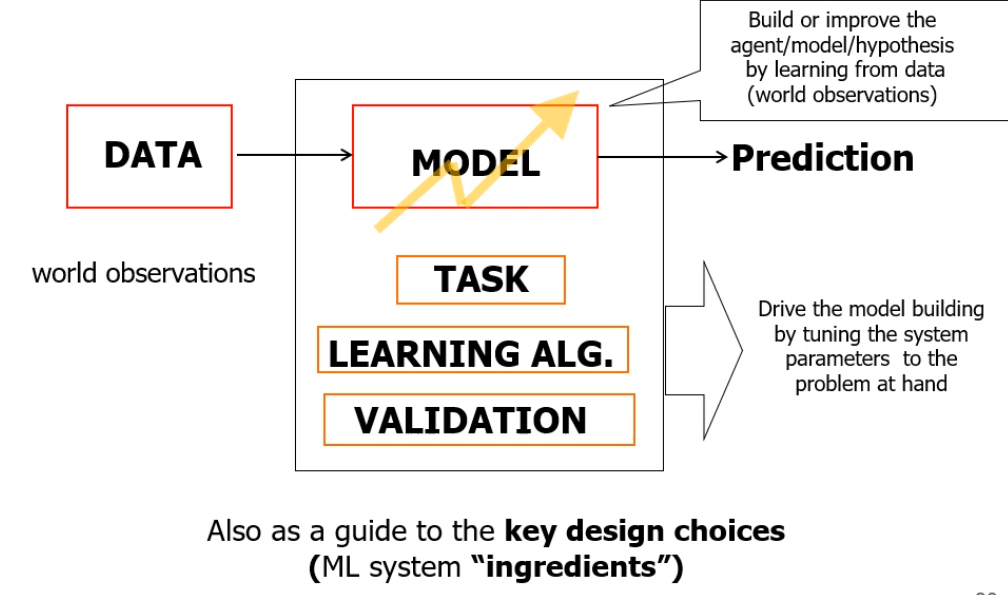
\includegraphics[scale=0.5]{1.png}
\end{center}
\subsection{Supervised learning} Given a set of training examples as $\langle$input, output$\rangle$ = $\langle x,d\rangle$ (\textbf{labeled examples}) for an unknown function $f$, find a \textit{good approximation} of $f$: an hypothesis $h$ that can be used for making predictions on unseen data $x'$.\\
The targets $d$ can be:
\begin{list}{}{}
	\item Discrete value, for \textbf{classification tasks}.\\
	$$f(x) \in \{1,2,\ldots,k\}$$\\
	\textbf{Patterns}, vectors of features, are seen as members of a class and the goal is to assign the new patterns observed to the correct class (or label)\\
	If the number of possible classes is two, then $f$ is a \textit{boolean function} and the task is called \textbf{binary classification} or \textbf{concept learning}: true or false, positive or negative, 0 or 1\ldots\\
	If the number of classes is $> 2$ then the task is a \textbf{multi-class classification task}. For example, categorizing images.
	\item Real value, for \textbf{regression tasks}.\\
	The patterns are seen as sets of variables (real values), and the task is a curve fitting task. The process aims to estimate a real-value function based of a finite set of noisy samples $\langle x, f(x) +$ random noise$\rangle$
\end{list}
\subsection{Unsupervised learning} No teacher. The training set is a set of unlabeled data $\langle x\rangle$. Examples: clustering, finding natural groupings in a set of data.
\subsection{Learning algorithm} Based on data, task and model: heuristic search, through the hypothesis space $H$, looking for the \textbf{best hypothesis}, the best approximation of the unknown target function, typically searching for the $h$ with the minimum \textit{error}. $H$ may not coincide with the set of all possible function and the search cannot be exhaustive, we need to make \textbf{assumpitons} (\textbf{inductive bias}).
\paragraph{Learning} Also called:
\begin{list}{}{}
	\item Inference, in statistics
	\item Adapting, in biology and systems
	\item Optimizing, in mathematics
	\item Training, in neural networks
	\item Function approximations, in mathematics
\end{list}
After introducing data, task, model and learning algorithm we will focus on: inductive bias, loss and concepts of generalization and validation.
\paragraph{Inductive bias} To set up a model we can (and need to) make assumptions about the nature of the target function, concerning either:
\begin{list}{}{}
	\item constraints in the model, \textbf{language bias} (in the hypothesis space $H$, due to the set of hypothesis that we can express or consider)
	\item constraints or preferences in learning algorithm/search strategy, \textbf{search bias} which is preferred
	\item or both
\end{list}
Such assumptions are needed to obtain an useful model for the ML aims, i.e. a model with generalization capabilities.\\
We can imagine learning a discrete function with discrete inputs assuming \textbf{conjunctive rules}, so using a \textbf{language bias} to work with a restricted hypothesis space.
\paragraph{Version Space} An hypothesis $h$ is consistent with the training set if $h(x) = d(x)$ for each training example $\langle x, d(x)\rangle$.\\
The \textbf{version space} $VS_{H, TR}$ is the subset of $H$ of the hypothesis consistent with all the training examples $\langle x, d(x)\rangle$ in the training set.\\
It's possible to do an exhaustive search in an efficient way, using clever algorithms. This means finding the set of all the hypothesis $h$ consistent with the training set. 
\paragraph{Unbiased Learner} The language bias (for example: using only conjunctive rules), may be \textbf{too restrictive}: if the target concept is $\not\in H$ then, obviously, it cannot be represented in $H$. We can use an $H$ that expresses every teachable concept (among propositions), that means that $H$ is the set of all possible subsets of $X$: the power set $\mathscr{P}(X)$. If $n = 10$ binary inputs, then $|X| = 2^{10} = 1024$ and $|\mathscr{P}(X)| = 2^{1024} = 10^{308}$ possible concepts, which is much more than the number of the atoms in the universe.\\
An unbiased learner is unable to generalize: the only examples that are unambiguously classified by an unbiased learner represented with the VS are the training examples themselves. Each unobserved instance will be classified positively by exactly half of the hypothesis in the VS and negative by the other half. Indeed: $\forall\: h$ consistent with $x_i$, $\exists\:h'$ identical to $h$ except $h'(x_i) \neq h(x_i)$, $h\in$ VS $\Rightarrow h'\in$ VS (because they are identical on the TR)
\paragraph{Why prefer the search bias?} In ML we use flexible approaches, expressive hypothesis spaces with universal generalization capability of the models, for example neural networks or decision trees. We avoid the language bias, so we do not exclude \textit{a priori} the unknown target function, but we focus on the search bias (ruled by the learning algorithm).
\paragraph{Loss} How to measure the quality of an approximation? We want to measure the distance between $h(x)$ and $d$, using a loss function/measure $L(h(x), d)$ for a pattern $x$ which has high value in cases of bad approximation. The error (or risk or loss) is an expected value of this $L$, for example $E(w) = \frac{1}{l}\sum_{p=1}^l L(h(x_p), d_p)$. Different $L$ for different tasks. Examples of loss functions:
\begin{list}{}{}
	\item Regression: $L(h(x_p), d_p) = (d_p - h(x_p))^2$, the squared error. MSE (mean squared error) over the data set
	\item Classification: $L(h(x_p), d_p) = \left\{\begin{array}{l l}
		0 & h(x_p) = d_p\\
		1 & else
	\end{array}\right.$
\end{list}
\paragraph{Learning and generalization} Learning: search for a \textbf{good function} in a function space from known data (typically minimizing an error/loss). \textbf{Good} with respect to generalization error: it measures how accurately the model predicts over novel samples of data (\textbf{measured over \underline{new} data}).\\
Generalization is the crucial point of ML. Performance in ML is the generalization accuracy or \textit{predictive accuracy} estimated by the error on the test set.
\paragraph{Phases}\begin{list}{}{}
	\item \textbf{Learning phase}: building the model, which includes training
	\item \textbf{Prediction phase}: evaluating the learned function over new never-seen-before samples (generalization capability)
\end{list}
\paragraph{Machine Learning issues} Inferring general functions from known data is an ill posed problem, which means that in general the solution is not unique because we can't expect the exact solution with finite data. What can we represent? And so, what can we learn?\begin{list}{}{}
	\item \textbf{Inductive learning hypothesis}: any $h$ that approximates $f$ well on training examples will also approximate $f$ well on new unseen instances $x$
	\item \textbf{Overfitting}: a learner overfits data if it outputs an hypothesis $h\in H$ having true/generalization error (risk) $R$ and empirical (training) error $E$, but there's another $h'\in H$ with $E' > E$ and $R' < R$, which means that $h'$ is the better one despite having a worse fitting on training data
\end{list}
\subsection{Statistical Learning Theory} Under what mathematical conditions is a model able to generalize? We want to investigate the generalization capability of a model, measured as a risk or test error, the role of the model complexity and the role of the number of data.\\
\textbf{Formal Setting}: approximate a function $f(\mathbf{x})$, with $d$ target ($d = f(\mathbf{x}) +$ noise), minimizing the \textbf{risk function} $$R = \int L(d, h(\mathbf{x}))\:dP(\mathbf{x},d)$$ which is the \textbf{true error over all the data}, given:
\begin{list}{}{}
	\item a value $d$ from the teacher and the probability distribution $P(\mathbf{x},d)$
	\item a loss function $L(h(\mathbf{x}),d) = (d - h(\mathbf{x}))^2$
\end{list}
We search for $h\in H\:|\: \min R$, but we only have the finite data set $TR = (\mathbf{x}_p, d_p)$ with $p = 1\ldots l$. Looking for $h$ means minimizing the empirical risk (the training error $E$), finding the best values for the model free parameters $$R_{emp} = \frac{1}{l}\sum_{p=1}^l (d_p - h(\mathbf{x}_p))^2$$
The inductive principle is the \textbf{ERM}, Empirical Risk Minimization: can we use $R_{emp}$ to approximate $R$?
\subsubsection{Vapnik-Chervonenkis dim and SLT} Given the VC dimension (simply VC), a measure of complexity of $H$ and by that we mean its flexibility to fit data.\\
The VC-bound states the following: it holds with probability $\frac{1}{\delta}$ that $$R \leq R_{emp} + \epsilon\left(\frac{1}{l}, \textsl{VC},\frac{1}{\delta}\right)$$
\begin{list}{}{}
	\item $\epsilon$ is a function called VC-confidence, that grows with VC and decreases with higher $l$ and $\delta$
	\item $R_{emp}$ decreases using complex models (with high VC)
	\item $\delta$ is the confidence, and it rules the probability that the bound holds.\\
	$\delta = 0.01 \Rightarrow$ the bound holds with probability $0.99$
\end{list}
Intuitively:
\begin{list}{}{}
	\item Higher $l$ (data) $\Rightarrow$ lower VC confidence and bound closer to $R$
	\item A too simple model, meaning with low VC, can be not sufficient due to high $R_{emp}$ (\textbf{underfitting})
	\item An higher VC with fix $l \Rightarrow$ lower $R_{emp}$, but VC and hence $R$ may increase (\textbf{overfitting})
\end{list}
\subsubsection{Structural risk minimization} Minimize the bound! There are different bounds formulations according to different classes of $f$, of tasks\ldots\\
In other words, we can make a good approximation of $f$ from examples, provided that we have a good number of data and the complexity of the model is suitable for the task.
\subsubsection{Complexity control} The Statistical Learning Theory allows for a formal framing of the problem of generalization and overfitting, providing an analytic upper bound to the risk $R$ for the prediction over all the data, regardless of the type of learning algorithm or the details of the model. So \textbf{the machine learning has good theoretical foundations}, the learning risk can be analytically limited and only a few concepts are fundamental. This leads to new models (such as the Support Vector Machine) and other methods that directly consider the control of the complexity in the construction of the model.
\subsection{Validation} Central role for the applications and the project. Two aims:
\begin{list}{}{}
	\item \textbf{Model Selection}: estimating the performance (\textbf{generalization error}) of different models in order to choose the best one. This includes searching for the best hyperparameters of the model.\\
	It returns a \textbf{model}.
	\item \textbf{Model Assessment}: with the final model, estimating/evaluating its prediction error/risk (\textbf{generalization error}) over new test data.\\
	It returns an \textbf{estimation}.
\end{list}
\textbf{Golden rule}: keep the two goals separated and use different datasets for each one.\\\\
In an ideal world, we'd have a large training set, a large validation set for model selection and a very large external unseen data test set. With finite and often small data sets we have just an estimation of the generalization performance. We have to use some techniques: hold-out and K-fold cross validation, for example.
\begin{list}{}{}
	\item \textbf{Hold-Out}: we partition the dataset $D$ into \textbf{training set} TR, \textbf{validation/selection set} VL and \textbf{test set} TS.\\
	All three are disjoint: TR is used to run the training algorithm, VL can be used to select the best model (hyperparameters tuning) and the \textbf{TS is only used for model assessment}.
	\begin{center}
		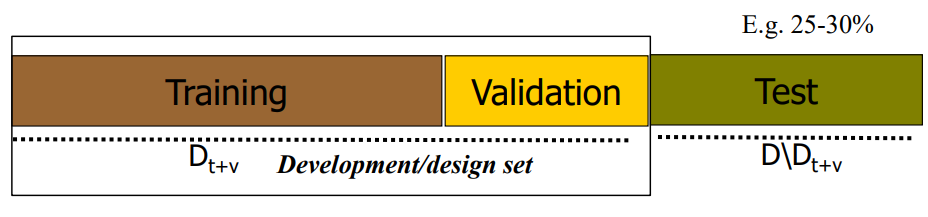
\includegraphics[scale=0.5]{2.png}
	\end{center}
	\item \begin{multicols}{2}
	\textbf{K-Fold}: this technique can make use of insufficient data. We split the dataset $D$ into $K$ mutually exclusive subsets $D_1,\ldots, D_k$, we train on $D - D_i$ and test it on $D_i$.\\
	This can be applied to both VL and TS splitting. Can be computationally very expensive and there's the issue of choosing the number of folds $K$.
	\begin{center}
		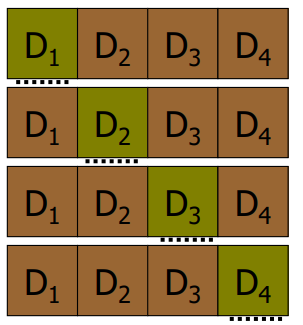
\includegraphics[scale=0.5]{3.png}
	\end{center}
	\end{multicols}
\end{list}
\pagebreak
\paragraph{Confusion Matrix} \begin{center}
	\begin{tabular}{|c|c|c|}
		\hline
		Actual/Predicted & \textbf{Positive} & \textbf{Negative}\\
		\hline
		\textbf{Positive} & TP & FN\\
		\hline
		\textbf{Negative} & FP & TN\\
		\hline
	\end{tabular}
\end{center}
\textbf{Specificity} = $\frac{\textsl{TN}}{\textsl{FP} + \textsl{TN}}$, and \textbf{true negative rate} $= 1 - \textsl{FPR}$\\
\textbf{Sensitivity} = $\frac{\textsl{TP}}{\textsl{TP} + \textsl{FN}}$, also known as \textbf{true positive rate} or \textbf{recall}\\
\textbf{Precision} = $\frac{\textsl{TP}}{\textsl{TP} + \textsl{FP}}$\\
\textbf{Accuracy}: \% of correctly classified patterns = $\frac{\textsl{TP + TN}}{\textsl{total}}$. Note that, for example, a 50\% accuracy on a binary classifier is equivalent to a random predictor.
\paragraph{ROC Curve} We plot \textbf{specificity} on \textbf{x-axis} and \textbf{sensitivity} on the \textbf{y-axis}. The diagonal corresponds to the worst classifier, the random guesser. Better curves have greater Area Under the Curve (AUC)
\begin{center}
	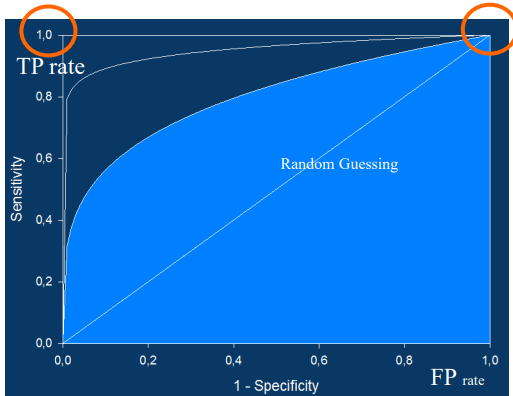
\includegraphics[scale=0.5]{50.png}
\end{center}
\subsection{Design Cycle}
\begin{center}
	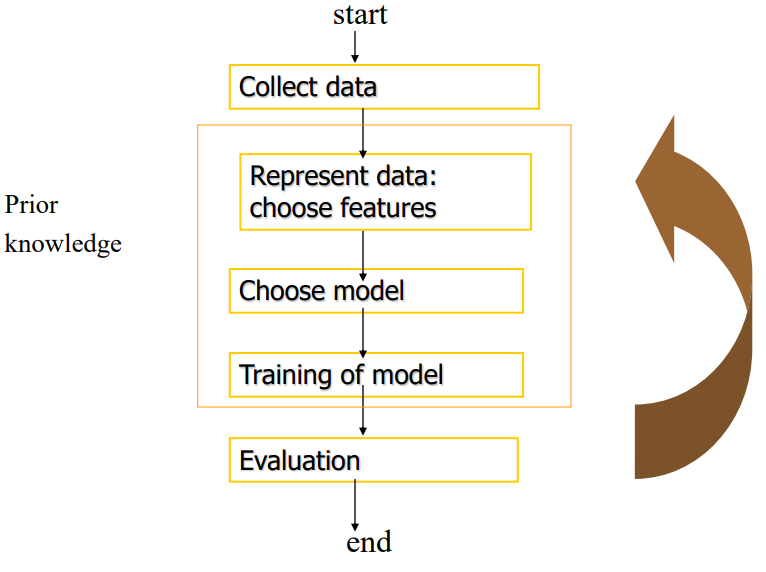
\includegraphics[scale=0.5]{52.png}
\end{center}
\begin{list}{}{}
	\item \textbf{Data Collection}: adequately large and representative set of examples for training and testing the system
	\item \textbf{Data Representation}: domain dependent, exploits prior knowledge of the application expert. It includes: feature selection, outliers detection, other preprocessing like variable scaling, missing data handling\ldots
	\item \textbf{Model Choice}: statement of the problem, hypothesis formulation (must know the limits of applicability of your model) and complexity control.
	\item \textbf{Bulding of the Model}: core of Machine Learning, through the learning algorithm and using the training data
	\item \textbf{Evaluation}: performance is predictive accuracy
\end{list}
\pagebreak
\subsection{Misinterpretations} For every statistical models, including Data Mining applications, causality if often assumed and a set of data representative of the phenomena is needed, so its no suitable for unrelated variables and for random phenomena like lotteries. Using uninformative input variables leads to poor modeling and poor learning results.\\
But causality cannot be inferred from data analysis alone, maybe there's statistical dependencies for reasons outside the data.\\
More specifically, in Machine Learning powerful model lead to higher risk, even for garbage data. Not well validated results can bring to a possibly misleading predicted outcome and interpretation.
\section{Linear Models} Mainstay of statistics.
\subsection{Univariate Linear Regression} Simple linear regression: we start with 1 input variable $x$ and 1 output variable $y$. We assume a model $h_w(x)$ expressed as $out = w_1x + w_0$ where $w$ are real-valued coefficients or \textbf{free parameters}, also called \textbf{weights}.\\
Given that the $w$s are continuously valued, we have an infinite hypothesis space but a nice solution from classical math. We can learn with this basic tool and, although simple, it includes many relevant concepts of modern Machine Learning and many methods in the field are based on this.
\paragraph{Least Mean Square} Learning means finding $w$ such that it minimizes the error/empirical loss, with best data fitting on the training set with $l$ examples.\\
So given a set of $l$ training examples $(x_p, y_p)$ with $p = 1,\ldots,l$, we have to find $h_w(x)$ in the form $w_1x + w_0$ that minimizes the expected loss on the training data. For the loss, we use the square of errors: \textbf{least mean square}, find $w$ to \textbf{minimize} the residual sum of squares.
$$Loss(h_w) = E(w) = \sum_{p=1}^l (y_p - h_w(x_p))^2 = \sum_{p=1}^l (y_p - (w_1x_p + w_0))^2$$
To have the mean, divide by $l$. How to solve? Local minimum as stationary point, so the gradient $\frac{\partial E(w)}{\partial w_i} = 0$ with $i = 1,\ldots,$ dim\_input $+1 = 1,\ldots, n+1$. For the simple linear regression (2 free parameters):
$$\frac{\partial E(w)}{\partial w_0} = 0\:\:\:\:\frac{\partial E(w)}{\partial w_1} = 0$$
$$\frac{\partial E(w)}{\partial w_i} = \frac{\partial(\:\overset{\text{delta}}{\overbrace{y-h_w(x)}}\:)^2}{\partial w_i} = 2(y-h_w(x))\frac{\partial(y-h_w(x))}{\partial w_i}=2(u-h_w(x))\frac{\partial (y-(w_1x+w_0))}{\partial w_i}$$
$$\frac{\partial E(w)}{\partial w_0} = -2(y - h_w(x))\:\:\:\:\frac{\partial E(w)}{\partial w_1} = -2(y - h_w(x))\cdot x$$
\paragraph{Notation} Assuming column vector for $\mathbf{x}$ and $\mathbf{w}$, in bold or without an index like $_i$.\\
$l$ is the number of data, $n$ is the dimension of input vector and $y_p,d_y$ or $t_p$ are targets with $p=1,\ldots,l$.
$$\mathbf{w}^T\mathbf{x} + w_0 = w_0 + w_1x_1+\ldots + w_nx_n = w_0 + \sum_{i=1}^n w_ix_i$$
$$w^Tx + w_0 = w_0 + w_1x_1+\ldots + w_nx_n = w_0 + \sum_{i=1}^n w_ix_i$$
$w_0$ is the threshold, bias, offset\ldots often we include $x_0=1$ as constant so that we can simply write $$\mathbf{w}^T\mathbf{x} = \mathbf{x}^T\mathbf{w}$$
$$w^Tx=x^Tw$$
$$h(\mathbf{x}_p)=\mathbf{x}_p^T\mathbf{w}=\sum_{i=0}^nx_{pi}w_i$$
\subsection{Classification} The same models used for regression can be used for classification: \textbf{categorical targets} $y$ or $d$, for example 0/1, -1/+1\ldots\\
We use an hyperplane ($\mathbf{wx}$) assuming negative or positive values. We exploit such models to decide if a point $\mathbf{x}$ belongs to the positive or the negative zone of the hyperplane to classify it. So we want to learn $\mathbf{w}$ such that we get a good classification accuracy. The decision boundary is $\mathbf{x}^T\mathbf{w} = \mathbf{w}^T\mathbf{x} = w_0 + w_1x_1 + w_2x_2 = 0$ and we can introduce a threshold function which can be written in many ways: \begin{list}{}{}
	\item $h(\mathbf{x}) = \left\{\begin{array}{c l}
	1 & \text{if }\mathbf{wx} + w_0 \geq 0\\
	0 & \text{else}
\end{array}	 \right.$
	\item $h(\mathbf{x}) = \text{sign}(\mathbf{wx} + w_0) = \text{sign}\left(\sum_{i=0}^n x_{pi}w_i\right)$
	\item \ldots
\end{list}
$w_0$ is called \textbf{threshold} or \textbf{bias}. $h(\mathbf{x}) = \mathbf{w}^T\mathbf{x} + w_0 \geq 0 \Leftrightarrow \mathbf{w}^T\mathbf{x} \geq -w_0$
\subsection{Learning Algorithms} Introducing 2 learning algorithms, both based on LSM and used for the linear model on regression and classification tasks. We start redefining the learning problem and the loss for them (in the case of $l$ data and multidimensional inputs).\\\\
\textbf{Learning problem for classification tasks}: given a set of $l$ training examples $(\mathbf{x}_p, y_p)$ and a loss function $L$, with $y_p \in \{0,1\}$ or $y_p \in \{-1, +1\}$, find the weight vector $\mathbf{w}$ that minimizes expected loss on the training data $$R_{emp} = \frac{1}{l}\sum_{p=1}^l L(h(\mathbf{x}_p), y_p)$$
The expected loss can be approximated by a smooth function. We can make the optimization problem easier by replacing the original objective function $L$ (0/1 loss) with a smooth, differentiable function: for example, the MSE loss (mean squared error).
\begin{center}
	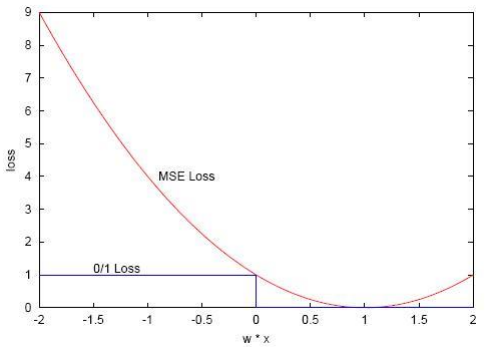
\includegraphics[scale=0.75]{4.png}
\end{center}
No classification error minimizing either 0/1 loss or MSE loss. Given $l$ training examples $(\mathbf{x}_p, y_p)$, find $\mathbf{w}$ that minimizes the residual sum of squares $$E(\mathbf{w})= \sum_{p=1}^l (y_p - \mathbf{x}_p^T \mathbf{w})^2 = ||\mathbf{y} - \mathbf{Xw}||^2$$
We can't use $h(\mathbf{x})$ in $E(\mathbf{w})$, as for regression, because $h(\mathbf{x}) = \text{sign}(\mathbf{w}^T \mathbf{x})$ is non-differentiable. Also, this is a quadratic function so the minimum always exists (but may not be unique). $\mathbf{X}$ is a $l\times n$ matrix with a row for each $\mathbf{x}_p$.
\paragraph{Direct Approach with a normal equation} Differentiating $E(\mathbf{w})$ with respect to $\mathbf{w}$ to get the \textbf{normal equation} $$(\mathbf{X}^T \mathbf{X})\mathbf{w} = \mathbf{X}^T \mathbf{y}$$
In the derivation we also find that $$\frac{\partial E(\mathbf{w})}{\partial w_j} = -2 \sum_{p=1}^l (\mathbf{x}_p)_j \cdot (y_p - \mathbf{x}_p^T \mathbf{w})$$
If $\mathbf{X}^T \mathbf{X}$ is not singular, then the unique solution is given by $$\mathbf{w} = (\mathbf{X}^T \mathbf{X})^{-1}\mathbf{X}^T \mathbf{y} = \mathbf{X}^+ \mathbf{y}$$ with $\mathbf{X}^+$ being the Moore-Penrose pseudoinverse. Else the solutions are infinite, so we can choose the $\min \text{norm}(\mathbf{w})$ solution.\\
The \textbf{Singular Value Decomposition} can be used for computing the pseudoinverse of a matrix ($\mathbf{X}^+$). With $$\mathbf{X} = \mathbf{U}\mathbf{\Sigma} \mathbf{V}^T \Rightarrow \mathbf{X}^+ = \mathbf{V}\mathbf{\Sigma}^+ \mathbf{U}^T$$ obtained by replacing every non-zero entry by its reciprocal.\\
We can apply SVD directly to compute $\mathbf{w} = \mathbf{X}^+ \mathbf{y}$, obtaining the minimal norm (on $\mathbf{w}$) solution of least squares problem.
$$\frac{\partial E(\mathbf{w})}{\partial w_j} = \frac{\partial \sum_{p=1}^l (y_p - \mathbf{x}_p^T \mathbf{w})^2}{\partial w_j} =$$
$$=\sum_{p=1}^l 2(y_p-\mathbf{x}_p^T\mathbf{w})\frac{\partial(y_p-\mathbf{x}_p^T\mathbf{w})}{\partial w_j} = \sum_{p=1}^l 2(y_p-\mathbf{x}_p^T\mathbf{w})\underset{\text{Only the component }j\text{ is not }0}{\left(0-\cancel{\frac{\partial\mathbf{x}_{p1}w_1}{\partial w_j}}-\cancel{\frac{\partial\mathbf{x}_{p2}w_2}{\partial w_j}}-\ldots-\frac{\partial\mathbf{x}_{pj}w_j}{\partial w_j}-\ldots-\cancel{\frac{\partial\mathbf{x}_{pn}w_n}{\partial w_j}}\right)}=$$
$$= \sum_{p=1}^l 2(y_p-\mathbf{x}_p^T\mathbf{w})\left(-\frac{\partial \mathbf{x}_{pj}w_j}{\partial w_j}\right)= -2 \sum_{p=1}^l (\mathbf{y}_p - \mathbf{x}_p^T \mathbf{w})(\mathbf{x}_p)_j$$
By imposing this $=0$ we can easily obtain the normal equation, first by sums then in matrix notations, obtaining the gradiend $E$. Another form, used in neural networks:
$$\frac{\partial E(\mathbf{w})}{\partial w_j}=-\sum_{p=1}^l 2 \underset{\delta_p}{\underbrace{(y_p-\mathbf{x}_p^T\mathbf{w})}} x_{pj} = -2\sum_{p=1}^l\delta_px_{pj}$$
\subsection{Gradient Descent} The derivation suggests an approach based on an iterative algorithm based on $$\frac{\partial E(\mathbf{w})}{\partial w_j} = -2 \sum_{p=1}^l (y_p - \mathbf{x}_p^T \mathbf{w})x_{pj}$$ The \textbf{gradient} is the \textbf{ascent direction}. We can move toward the minimum with a gradient descent $\Delta \mathbf{w} = -$ gradient of $E(\mathbf{w})$. \textbf{Local search}: we begin with a initial weight vector and modify it iteratively to minimize the error function. The gradient vector is
$$\Delta \mathbf{w} = -\frac{\partial E(\mathbf{w})}{\partial \mathbf{w}} = \left[\begin{array}{c}
-\frac{\displaystyle\partial E(\mathbf{w})}{\displaystyle\partial w_1}\\\vdots\\-\frac{\displaystyle\partial E(\mathbf{w})}{\displaystyle\partial w_n}
\end{array}\right] = \left[\begin{array}{c}
\Delta w_1\\\vdots\\\Delta w_n
\end{array} \right]$$
Allowing us to work in a multi dimensional space without the need to visualize it. Hence, the iterative approach will move using a learning rule based on a "delta" of $w$ proportional to the opposite of the local gradient. The movements will be made according to $$\mathbf{w}_{new} = \mathbf{w} + \eta\cdot\Delta \mathbf{w}$$
The simple algorithm is as follows:
\begin{enumerate}
	\item Start with weight vector $\mathbf{w}_{initial}$ and fix $0 < \eta < 1$
	\item Compute $\Delta \mathbf{w} = -$ gradient of $E(\mathbf{w}) = -\frac{\partial E(\mathbf{w})}{\partial \mathbf{w}}$ (or for each $w_i$)
	\item Compute $\mathbf{w}_{new} = \mathbf{w} + \eta\cdot\Delta \mathbf{w}$ (or for each $w_i$)\\
	$\eta$ is the step size or \textbf{learning rate}
	\item Repeat from $2$ until convergence or $E(\mathbf{w})$ sufficiently small
\end{enumerate}
\subsubsection{Batch version} The gradient is the sum over all the $l$ patterns. Provides a more precise evaluation of the gradient over $l$ data. We upgrade the weight after the sum
$$\frac{\partial E(\mathbf{w})}{\partial w_j} = -2 \sum_{p=1}^l (y_p - \mathbf{x}_p^T \mathbf{w})x_{pj}$$
\subsubsection{Online/Stochastic version} We upgrade the weights with the error that is computed for each pattern. Hence, the second pattern output is based on weights already updated from the first and so on. In makes progress with each example it sees. Can be faster, but needs smaller $\eta$
$$\frac{\partial E_p(\mathbf{w})}{\partial w_j} = -2(y_p - \mathbf{x}_p^T \mathbf{w})x_{pj} = -\Delta_p w_j$$
\subsubsection{Gradient Descent as error correction delta rule} The error correction rule, also called Widrow-Hoff or delta rule, changes $w_j$ proportionally to the error (target $y$ $-$ output)
$$\Delta w_j = 2 \sum_{p=1}^l x_{pj} (y_p - \mathbf{x}_p^T \mathbf{w})$$
$$\mathbf{w}_{new} = \mathbf{w} + \eta\cdot\Delta \mathbf{w}$$
We improve by learning on previous errors.
\subsection{Extending the linear model}
\paragraph{Inductive Bias}
Gradient descent is a simple and effective local search approach to a LMS solution. It allows to search through an infinite hypothesis space, can be easily applied for continuous $H$ and differentiable losses and isn't only for linear models (also neural networks and deep learning models).\\
Many possible improvements (Newton, quasi-Newton methods, conjugate gradients\ldots)
\begin{list}{}{}
	\item \textbf{Language bias}: $H$ is a set of linear functions.
	\item \textbf{Search Bias}: ordered search guided by the least squares minimization goal.\\
	For instance, we could prefer a different method to obtain a restriction on the values of parameters, achieving a different solution with other properties.
\end{list}
Shows that even for a simple model there are many possibilities. We still need a principled approach.
\subparagraph{Limitations} In geometry, two set of points are linearly separable in an $n$-dimensional space if they can be separated by a $(n-1)$-dimensional hyper-plane. In 2 dimensions, if they can be separated by a line, in 3 dimensions, by a plane\ldots\\
The linear decision boundary can provide exact solutions only for linearly separable sets of points.
\paragraph{Extending} Note that linear refers to the way in which $\mathbf{w}$, the regression coefficient, occur in the regression equation. So we can use transformed inputs, such as $x, x^2, x^3\ldots$ with a \textbf{non-linear relationship between inputs and output}, maintaining the learning machinery used so far. $$h_\mathbf{w}(\mathbf{x}) = w_0 + w_1 x + w_2 x^2 + \ldots + w_M x^M = \sum_{j=0}^M w_j x^j$$
\paragraph{Linear Basis Expansion} (LBE) $$h_\mathbf{w}(\mathbf{x}) = \sum_{k=0}^K w_k\phi_k(\mathbf{x})$$
$$\phi_k : \mathbb{R}^n \rightarrow \mathbb{R}$$
Augments the input vector with additional variables which are transformations of $\mathbf{x}$ according to a function $\phi_k : \mathbb{R}^n \rightarrow \mathbb{R}$, so number of parameters $K > n$: linear in the parameters, so we can use the same learning algorithms as before.
\begin{list}{}{Examples are:}
	\item Polynomial representation of $\mathbf{x}$: $\phi(\mathbf{x}) = x_j^2, \phi(\mathbf{x} = x_jx_i,\ldots$
	\item Non-linear transformation of single inputs: $\phi(\mathbf{x})=\log(x_j), \phi(\mathbf{x})=\sqrt{x_j},\ldots$
	\item Non-linear transformation of multiple inputs: $\phi(\mathbf{x})=\|\mathbf{x}\|,\ldots$
	\item Splines,\ldots
\end{list}
Which $\phi$? Towards the \textbf{dictionary approaches}. Pro: can model more complicated relationships than linear, so it's more expressive. Cons: with large basis of functions, we easily risk overfitting, hence we require \textbf{controlling the complexity} (as in flexibility of the model to fit the data). How to do that? Many approaches\ldots
\subparagraph{Ridge Regression} (or \textbf{Tikhonov Regularization}): smoothed model, a \textbf{coefficient shrinkage} approach to model complexity control.\\
	Add constraints to the sum of value of $|w_j|$, penalizing models with high values of $|w|$ (so favoring sparse models, using less terms due to weights $w_j = 0$ or close)
	$$Loss(\mathbf{w}) = \sum_{p=1}^l (y_p - \mathbf{x}_p^T \mathbf{w})^2 + \lambda||\mathbf{w}||^2$$ with $\lambda$ being the \textbf{regularization hyper-parameter}. It implements the control of the model complexity, leading to a model with less VC-dim with a trade-off controlled through a single parameter, $\lambda$.
\begin{list}{}{}
	\item Thikonov uses $||\:||_2$
	\item Lasso uses $||\:||_1$
	\item Elastic nets uses both $||\:||_1$ and $||\:||_2$
\end{list}
Solving Tikhonov Regularization:
\begin{list}{}{}
	\item Direct approach
	$$\mathbf{w} = \underset{\text{Always invertible}}{\underbrace{(\mathbf{X}^T\mathbf{X}+\lambda\mathbf{I})^{-1}}}\mathbf{X}^T\mathbf{y}$$
	\item Gradient approach
	$$\mathbf{w}_{new} = \mathbf{w}+\eta\cdot\Delta\mathbf{w} - 2\lambda\mathbf{w}$$
	\textbf{Weight decay} technique, basically adds $2\lambda\mathbf{w}$ to the gradient: with 0 gradient, it decreases the value of each $w_j$ with a fraction of the old $w_j$
\end{list}
The penalty term penalizes high values of the weights and tends to drive all them to smaller values, with some to zero. It implements a control of the model complexity, leading to a model with less, or proper, VC-dim with a \textbf{trade-off obtained with just one parameter} that you can control: $\lambda$.
\paragraph{Learning Timing} \begin{list}{}{}
	\item \textbf{Eager}: analyze data and construct an explicit hypothesis
	\item \textbf{Lazy}: store training data and wait test data point, then construct an ad hoc hypothesis.
\end{list}
\pagebreak
\subsection{K-NN}
The algorithm is simple: store the training data $\langle\mathbf{x}_p, y_p\rangle$ and given an input $\mathbf{x}$ find the $k$ nearest training examples $\mathbf{x}_i$, then output the mean label.
$$\text{avg}_k(\mathbf{x})=\frac{1}{k}\sum_{\mathbf{x}_i\in N_k(\mathbf{x})}y_i$$
$N_k(\mathbf{x})$ is a neighborhood of $\mathbf{x}$ that contains exactly $k$ neighbors, closest according to $d$. Thus the classification rule is the majority voting among the members of $N_k(\mathbf{x})$
$$h(\mathbf{x})=\left\{\begin{array}{c l}
1&\text{if }\text{avg}_k(\mathbf{x})>0.5\\
0&\text{else}
\end{array}\right.$$
For the regression tasks we use directly the $\text{avg}$: mean over the $k$ nearest neighbors ($k$-NN)
\paragraph{Nearest} For example: Euclidean distance
$$d(\mathbf{x},\mathbf{x}_p)=\sqrt{\sum_{t=1}^n(x_t-x_{pt})^2}=\|\mathbf{x}-\mathbf{x}_p\|$$
\subparagraph{Voronoi Diagram} Each cell consists of points closer to $x$ than any other patterns. The segments are all points in plan equidistant to two patterns. It is implicitly used by K-NN.
\paragraph{Multiclass} Return the most common class among its $k$ nearest neighbors: we count the classes in the neighbor (with $\mathbf{1}_{v,y_i}$) taking the most frequent (with$\arg\max_v$)
$$h(\mathbf{x})=\arg\max_v\sum_{\mathbf{x}_i\in N_k(\mathbf{x})}\mathbf{1}_{v,y_i}$$
$$\mathbf{1}_{v, y_i}=\left\{\begin{array}{c l}
1&\text{if }v = y_i\\
0&\text{else}
\end{array}\right.$$
\subparagraph{Weighted Distance} It can be useful to weight the contributions of the neighbors, so that the nearer neighbors contribute more to the average than the more distant ones.
$$h(\mathbf{x})=\arg\max_v\sum_{\mathbf{x}_i\in N_k(\mathbf{x})}\mathbf{1}_{v,y_i}\cdot\frac{1}{d(\mathbf{x},\mathbf{x}_i)^2}$$
$$\mathbf{1}_{v, y_i}=\left\{\begin{array}{c l}
1&\text{if }v = y_i\\
0&\text{else}
\end{array}\right.$$
\paragraph{K-NN vs linear} Two extremes of the ML panorama:
\begin{center}
	\begin{tabular}{l | l}
		\textbf{Linear} & \textbf{K-NN}\\
		\hline
		Rigid (low variance) & Flexible (high variance)\\
		Eager & Lazy\\
		Parametric & Instance-Based
	\end{tabular}
\end{center}
K-NN represents an extreme. There's no global hypothesis for all the instances, so no model to fit: we need to memorize all the input examples. Local estimations (by locally constant functions) versus the linear global approximation/estimation of the target function over the instance space.\\
It's a lazy, memory-based, instance-based, distance-based method.
\subparagraph{Bayes Error Rate} If we know the density $P(x,y)$, we classify the most probable class, using the conditional distribution as: output the class $v\:|\:$ is $\max P(v\:|\:x)$, the \textbf{Bayes Classifier}.\\
The error rate of this classifier is called the \textbf{Bayes error rate}: the \textbf{minimum achievable error rate given the distribution of the data}. K-NN directly approximates this solution (majority vote in a nearest neighborhood) except that conditional probability is relaxed to conditional probability withing a neighborhood and probabilities are estimated by training sample proportions
\subparagraph{Inductive bias of K-NN} The assumed distance tells us which are the most similar examples. The classification is assumed similar to the classification of the neighbors according to the assumed metric.
\subparagraph{Limitations} The \textbf{computational cost is deferred to the prediction phase}: makes the local approximation to the target function for each new example to be predicted.\\
\textbf{High retrieval cost}: computationally intensive, in time, for each new input because computes the distance from the test sample to all stored vectors, so high cost in space too (all training data).\\
It provides a good approximation if we can find a significant set of data close to any $x$. \textbf{Can fail when we have a lot of input variables} (high $n$, high dimensionality) due to the curse of dimensionality:
\begin{list}{}{}
	\item \textbf{Hard to find nearby points} in high dimensions\\
	K-NN can fail in high dimensions because it becomes difficult to gather $K$ observation close to a target point $x_q$: near neighborhoods tend to be spatially large and estimates are no longer local
	\begin{center}
		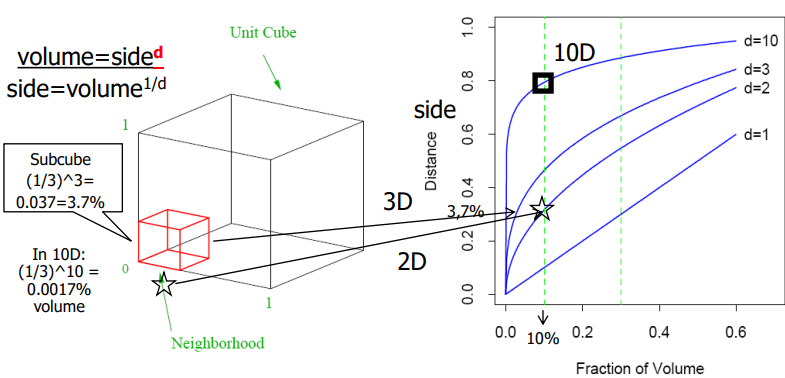
\includegraphics[scale=0.75]{5.png}
	\end{center}
	\item \textbf{Low sampling density} for high-dim data\\
	Sampling density is proportional to $l^{\frac{1}{d}}$ with $l$ data and $d$ data dim. If 100 points are needed to estimate a function in $\mathbb{R}$ (1 dim), then $100^{10}$ are needed in $\mathbb{R}^{10}$
	\item Irrelevant features: the \textbf{curse of noisy}\\
	If the target depends only on a few features in $x$, we could retrieve a similar pattern with the similarity dominated by the large number of irrelevant features. This grows with dimensionality. We may weight features according to the relevance, or adopt feature selection approaches (eliminating some variables)
\end{list}
\pagebreak
% ML-21-NN-part1-v.0.1.pdf
\section{Neural Networks} Models used to:
\begin{list}{}{}
	\item Study and model biological systems and learning processes (biological realism is essential)
	\item Introduce effective machine learning systems and algorithms (often losing a strict biological realism, but machine learning, computational and algorithmic properties are essential)
\end{list}
For us, these are called \textbf{Artificial Neural Networks} (ANN): a flexible machine learning tool in the sense of approximating functions (builds a mathematical function $h(x)$ with special properties). A neural network:
\begin{list}{}{}
	\item Can learn from examples
	\item Are \textbf{universal approximators} (\textbf{Theorem of Cybenko}): flexible approaches for arbitrary functions (including non-linear)
	\item Can deal with noisy and incomplete data, with a graceful degradation of performance
	\item Can handle continuous and discrete data for both regression and classification tasks
	\item It's a \textbf{paradigm}: it encompasses a wide set of models
\end{list}
\subsection{Artificial Neuron} Input from external source or other units, with weights $\mathbf{w}$ as free parameters: can be modified by the learning process. The unit $i$ computes $f(\sum_j w_{ij}x_j)$ with $w_{ij}$ the weight from input $j$ to unit $i$. $f$ is called \textbf{activation function}: linear, threshold or logistic (sigmoid). The weighted sum $\sum_j w_{ij}x_j$ is called net input to unit $i$, or $net_i$.
\begin{center}
	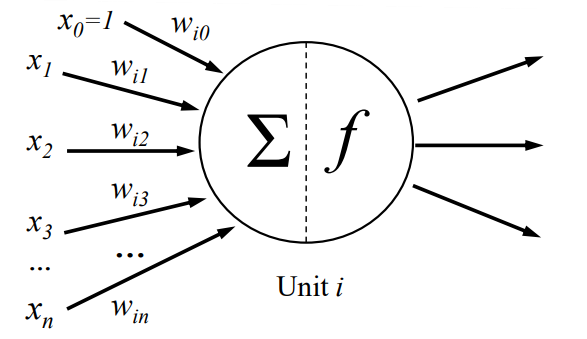
\includegraphics[scale=0.75]{6.png}
\end{center}
A neuron can either be firing (1) or not firing (0). All connections are equivalent and characterized by a real number (their strength $\mathbf{w}_{ij}$), which is positive of excitatory connections and negative for inibitory connections. A neuron $i$ becomes active when the sum of those connections $w_{ij}$ coming from neurons $j$ plus a bias is larger than zero.\\
Three types of activation functions:
\begin{list}{}{}
	\item \textbf{Linear}, or identity: $f(x) = x$
	\item \textbf{Threshold}, for the \textbf{perceptrons}: $f(x) = \text{sign}(x)$
	\item \textbf{Logistic}: $f(x) = \frac{1}{1 + e^{-\alpha x}}$
\end{list}
\subsubsection{Perceptron} A neuron that uses a threshold as activation function. Can be composed and connected to build a network: \textbf{MLP}, Multi Layer Perceptron 
\subparagraph{Xor} $x_1 \oplus x_2 = x_1\cdot \overline{x_2} + \overline{x_1}\cdot x_2$. Let $h_1 = x_1\cdot x_2, h_2 x_1 + x_2$ then $x_1 \oplus x_2 = \overline{h_1} \cdot h_2$ with $\wedge = \cdot$ and $\vee = +$.\\
So two layers are sufficient, but single layer cannot model all functions due to limits of single perceptron and the linear separable problems.
\paragraph{Hidden Representation} Developing high level hidden features is a key factor in NN. The representation in the hidden layer makes the task easier for the output layer. Such composition of sub/intermediate operations to perform a complex task can be extended through many layers of abstraction, and in NNs such \textbf{internal representation} (intermediate features) \textbf{can be learned}.
\paragraph{Learning for one unit model} \begin{list}{}{}
	\item \textbf{Adaline}, adaptive linear neuron: LMS direct solution and gradient descent solution
	\item \textbf{Perceptron}, non linear: only classification.\\
	Minimize number of misclassified patterns, find $\mathbf{w}\:|\:sign(\mathbf{w}^T\mathbf{x}) = d$. Online algorithm, a step can be made for each input pattern.
	\begin{enumerate}
		\item Initialize weights
		\item Pick learning rate $\eta$ (between 0 and 1)
		\item Until stopping condition (e.g.: weights don't change):
		\begin{list}{}{}
			\item For each training pattern $(\mathbf{x}, d)$ compute output activation $out = sign(\mathbf{w}^T \mathbf{x})$.\\
		If $out = d$ then don't change weights\\
		If $out \neq d$ update weights $\mathbf{w}_{new} = \mathbf{w} + \eta\cdot d\cdot \mathbf{x}$ adding $+\eta \mathbf{x}$ if $\mathbf{wx}\leq 0$ and $d = +1$ or $-\eta \mathbf{x}$ if $\mathbf{wx} > 0$ and $d = -1$.\\Different form: $\mathbf{w}_{new} = \mathbf{w} + \frac{1}{2}\cdot\eta\cdot (d-out)\cdot \mathbf{x}$
		\end{list}
	\end{enumerate}
	The first is called \textbf{Hebbian learning} form $$\mathbf{w}_{new} = \mathbf{w} + \eta d \mathbf{x}$$ while the second is the \textbf{error correction learning} form $$\mathbf{w}_{new} = \mathbf{w} + \frac{1}{2}\eta (d-out) \mathbf{x}$$
	It's a recall from LMS: a error correction/delta/Widrow-Hoff/Adaline/LMS rule that changes the $\mathbf{w}$ proportionally to the error (target $d -$ output).\\
	In terms of neurons, the adjustment made to a synaptic weight is proportional to the product of error signal and the input signal that excite the synapse. Easy to compute when errors signal $\delta$ is directly measurable (meaning that we know the desired response for each unit).
\end{list}
\paragraph{Perceptron Convergence theorem} A perceptron can represent linear decision boundaries, so it can solve linearly separable problems. Also, it can always learn the solution with the perceptron learning algorithm.\\
The \textbf{perceptron convergence theorem} is a milestone: a biologically inspired model with well-defined and proved computational capabilities and proved by a theorem. It states that \textbf{the perceptron is guarateed to converge} (classifying correctly all the input patterns) \textbf{in a finite number of steps if the problem is linearly separable}. This independently of the starting point, although the final solution is not unique and it depends on the starting point.
\subparagraph{Preliminaries} We sometimes omit $^T$ for the dot product $\mathbf{w}^T \mathbf{x}$
\begin{list}{}{}
	\item We focus on positive patterns, assuming $(\mathbf{x}_i, d_i)\in$ TR set with $d_i = +1$ or $-1$
	\item Linearly separable $\Rightarrow\exists\: \mathbf{w}^*$ solution $|\:d_i(\mathbf{w}^* x_i)\geq \alpha = \min_i d_i(\mathbf{w}^*\mathbf{x}_i) > 0$, hence $\mathbf{w}^*(d_i\mathbf{x}_i)\geq \alpha$
	\item $\mathbf{x}_i' = (d_i\mathbf{x}_i)$ then $\mathbf{w}^*$ solution $\Leftrightarrow \mathbf{w}^*$ solution of $(\mathbf{x}_i', +1)$\\
	This because:
	\begin{list}{}{}
		\item If $\mathbf{w}^*$ solves $\Rightarrow d_i(\mathbf{w}^*\mathbf{x}_i) \geq \alpha \Rightarrow (\mathbf{w}^*d_i\mathbf{x}_i)\geq\alpha\Rightarrow (\mathbf{w}^*\mathbf{x}_i')\geq\alpha \Rightarrow \mathbf{w}^*$ solution of $(\mathbf{x}_i', +1)$
		\item If $\mathbf{w}^*$ is a solution of $(\mathbf{x}_i', +1)\Rightarrow(\mathbf{w}^*d_i\mathbf{x}_i)\geq \alpha\Rightarrow d_i(\mathbf{w}^*\mathbf{x}_i)\geq \alpha\Rightarrow \mathbf{w}^*$ solves for $\mathbf{x}_i$
	\end{list}
	\item Also assuming $\mathbf{w}(0) = 0$ (at step $0$), $\eta = 1$ and $\beta = \max_i |x_i|^2$ where $|\:|$ is the euclidean norm
	\item After $q$ errors (all false negatives), $$\mathbf{w}(q) = \sum_{j=1}^q \mathbf{x}_{i_j}$$ with $_{i_j}$ denoting the patterns belonging to the subset of misclassified patterns and $\mathbf{w}(j) = \mathbf{w}(j-1)  + \mathbf{x}_{i_j}$
	\item Rule: $\mathbf{w}_{new} = \mathbf{w}+\eta d\mathbf{x}$ with $d=+1$ because all positive patterns
\end{list}
\subparagraph{Proof} The basic idea is that we can find lower and upper bound to $|\mathbf{w}|$ as a function of $q^2$ steps (lower bound) and $q$ steps (upper bound) $\Rightarrow$ we can find the number of steps $q\:|$ the algorithm converges.\\\\
Lower bound on $|\mathbf{w}(q)|$ is $$\mathbf{w}^* \mathbf{w}(q) = \mathbf{w}^*\sum_{j=1}^q \mathbf{x}_{ij}\geq q\alpha$$ recalling that $\alpha=\min_i\:(\mathbf{w}^*\mathbf{x}_i)$.\\
With Cauchy-Schwartz we know that $(\mathbf{wv})^2 \leq |\mathbf{w}|^2|\mathbf{v}|^2$ where $|\mathbf{w}|^2 = ||\mathbf{w}||_2 ^2$
$$|\mathbf{w}^*|^2|\mathbf{w}(q)|^2 \geq (\mathbf{w}^*\mathbf{w}(q))^2 \geq (q\alpha)^2 \Rightarrow |\mathbf{w}(q)|^2 \geq \frac{(q\alpha)^2}{|\mathbf{w}^*|^2}$$
Also, because $|\mathbf{a} + \mathbf{b}|^2 = |\mathbf{a}|^2 + 2\mathbf{ab} + |\mathbf{b}|^2$
$$|\mathbf{w}(q)|^2 = |\mathbf{w}(q-1)+ \mathbf{x}_{i_q}|^2 = |\mathbf{w}(q-1)|^2 + 2\mathbf{w}(q-1)\mathbf{x}_{i_q} + |\mathbf{x}_{i_q}|^2$$
For the $q$-th error, $2\mathbf{w}(q-1)\mathbf{x}_{i_q} < 0$, so $$|\mathbf{w}(q)|^2 \leq |\mathbf{w}(q-1)|^2 + |\mathbf{x}_{i_q}|^2$$ and by iteration, given $\mathbf{w}(0) = 0$, we have $$|\mathbf{w}(q)|^2 \leq \sum_{j=1}^q |\mathbf{x}_{i_j}|^2 \leq q\beta$$ with $\beta = \max_i |\mathbf{x}_i|^2$
So we have an upper bound $q\beta$ and a lower bound $\frac{(q\alpha)^2}{|\mathbf{w}^*|^2}$, so $$\underset{\text{Upper bound}}{q\beta}\geq |\mathbf{w}(q)|^2\geq \underset{\text{Lower bound}}{\frac{(q\alpha)^2}{|\mathbf{w}^*|^2}}$$ $$q\beta\geq q^2\alpha'$$ $$\beta\geq q\alpha'$$ $$q \leq \frac{\beta}{\alpha'} = \frac{\max_i |\mathbf{x}_i|^2}{\min_i\:(\mathbf{w}^*\mathbf{x}_i)}$$
\paragraph{Differences}
	$$\mathbf{w}_{new} = \mathbf{w} + \eta(d-\text{out})\mathbf{x}$$
Apparently similar but:
\begin{multicols}{2}
	\begin{list}{}{\textbf{LMS algorithm}}
		\item LSM rule derived without threshold activation functions
		\item Hence for training $\delta = d - \mathbf{w}^T\mathbf{x}$
		\item Can still be used for classification using\\$h(\mathbf{x}) = \text{sign}(\mathbf{w}^T \mathbf{x})$, LTU
		\item Minimizes $E(\mathbf{w})$ ($\text{out} = \mathbf{w}^T\mathbf{x}$)
		\item Asymptotic convergence also for not linear separable problems
		\item Not always zero classification errors
		\item Can be extended to network of units (NN) using the gradient based approach
	\end{list}
	\begin{list}{}{\textbf{Perceptron learning algorithm}}
		\item Perceptron uses out $= \text{sign}(\mathbf{w}^T\mathbf{x})$
		\item versus $\delta = d - \text{sign}(\mathbf{w}^T\mathbf{x})$
		\item
		\item Minimizes misclassifications ($\text{out} = \text{sign}(\mathbf{w}^T\mathbf{x})$)
		\item Always converges in a finite number of steps for a linear separable problem to a perfect classifier\\
		Else it doesn't converge
		\item 
		\item Difficult to be extended to network of units (NN)
	\end{list}
\end{multicols}
\paragraph{Activation functions}
\begin{list}{}{}
	\item \textbf{Linear}, or identity: $f(x) = x$
	\item \textbf{Threshold}, for the \textbf{perceptrons}: $f(x) = \text{sign}(x)$
	\item \textbf{Logistic}: $f(x) = \frac{1}{\displaystyle 1 + e^{-\alpha x}}$\\
	This is a non-linear squashing function like the sigmoidal logistic function: it assumes a continuous range of values in the bounded interval $[0,1]$. It has the property of being a smoothed differentiable threshold function, with $\alpha$ being the slope parameter of the sigmoid function.
	\item Tanh-like, piecewise linear approximation for efficient computation
	\item \textbf{ReLU}, rectifier $f(x)=\max(0, x)$
	\item Softplus, smooth approximation of the ReLU $f(x)=\ln(1+e^x)$
	\item \textbf{Radial basis}: $f(x) = e^{-\alpha x^2}$
	\item \textbf{Softmax}
	\item \textbf{Stochastic neurons}, where the output is +1 with probability $P(net)$ or -1 with $1-P(net) \Rightarrow$ Boltzmann machines and other models rooted in statistical mechanics.
\end{list}
For the derivatives, a step function has no derivative, which is exactly why it isn't used. The sigmoids have ($\alpha = 1$): for the asymmetric case $$\frac{df_\sigma(x)}{dx} = f_\sigma(x) (1-f_\sigma(x))$$ and for the symmetric case $$\frac{df_{tanh}(x)}{dx} = 1 - f_{tanh}(x)^2$$ 
The sigmoid logistic function has the property of being a smoothed \textit{differentiable} threshold function. Hence, we can derive a Least (Mean) Square algorithm, by computing the gradient of the mean square loss function as for the linear units (also for a classifier).\\
From $\text{out}(\mathbf{x}) = \mathbf{x}^T\mathbf{w}$ to $$\text{out}(\mathbf{x}) = f_\sigma(\mathbf{x}^T\mathbf{w})$$ where $f_\sigma$ is a logistic function. Find $\mathbf{w}$ that minimizes the residual sum of squares $$E(\mathbf{w}) = \sum_p (d_p - \text{out}(\mathbf{x}_p))^2 = \sum_p (d_p - f_\sigma(\mathbf{x}_p^T\mathbf{w}))^2$$
$$\frac{\partial E(w)}{\partial w_j} = -2\sum_p^l x_{pj} (d_p - f_\sigma(\mathbf{x}_p^T\mathbf{w}))f'_\sigma(\mathbf{x}_p^T\mathbf{w}) =$$ $$= -2\sum_p^lx_{pj}\underset{\text{new }\delta_p}{\underbrace{\delta_pf'_\sigma(\text{net}(\mathbf{x}_p))}}$$
This for 1 unit and patterns $p = 1\ldots l$.\\
The same as for linear unit using the new delta rule
$$\mathbf{w}_{new}=\mathbf{w}+\eta\delta_p\mathbf{x}_p$$
$$\delta_p = (d_p - f_\sigma(\text{net}(\mathbf{x}_p)))f'_\sigma(\text{net}(\mathbf{x}_p)) = (d_p-\text{net}(\mathbf{x}_p))f'_\sigma$$
Again an error correction rule.
\paragraph{Neural Network} In an MLP architecture: units connected by weighted links, organized in layers:
\begin{list}{}{}
	\item input layer, source of the input $\mathbf{x}$. Copies the source external input patterns $\mathbf{x}$, without computing $\text{net}$ and $f$.
	\item hidden layer, projects onto another hidden or an output layer, computing.
\end{list}
Can be viewed as network of units or a flexible function:
$$h(\mathbf{x}) = f_k\left(\sum_j w_{kj}f_j\left(\sum_i w_{ji}x_i\right)\right)$$
As for notation, given
\begin{center}
	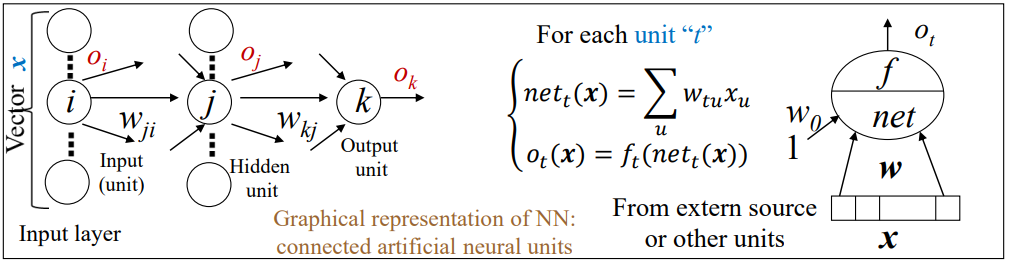
\includegraphics[scale=0.6]{7.png}
\end{center}
We have that the index $t$ denotes a generic unit, can be either $k$ or $j$. $u$ denotes a generic input component, either $i$ or $j$.\\
$x$ is a generic input from an external source (input vector) or from other units according to the position of the unit in the network. If we load the pattern $x$ in the input layer, we can use the notation with $o$ for both the inputs and the hidden units outputs. Hence, inside the network, the input to each unit $t$ from any source $u$ (through the connection $w_{tu}$) is typically denoted as $o_u$.
\subparagraph{Architectures}
\begin{list}{}{}
	\item \textbf{Feedforward NN} Standard architecture of the NNs. Direction: input $\longrightarrow$ output
	\item \textbf{Recurrent NN} adds feedback loops connections to the network topology. These self-loop connections provide the network with dynamical properties, leaving a "memory" of the past computations inside the model. This allows us to extend the representation capability of the model to the processing of sequences and structured data.
\end{list}
\subparagraph{Flexibility} The hypothesis space is a \textbf{continuous space} of all the functions that can be represented by assigning the weight values of the given architecture. Depending on the class of values produced by the output units (discrete or continuous), the model can deal, respectively, with classification tasks (sigmoidal output $f$) or regression tasks (linear output $f$). Also multi-class and multi-regression, with multiple output units.\\
A NN can be seen either as:
\begin{list}{}{}
	\item A \textbf{function}, \textbf{non-linear in the parameters} $\mathbf{w}$ $$h(\mathbf{x}) = f_k\left(\sum_j w_{kj}\:\underset{\text{Unit}}{\underbrace{f_j\left(\sum_i w_{ji}x_i\right)}}\right)$$
	with each $f_j\left(\sum_i w_{ji}x_i\right)$ computed by an independent processing element (unit)
	\item A \textbf{dictionary approach}, as an adaptive basis function approach. $$\phi_j(\mathbf{x},\mathbf{w})=f_j\left(\sum_i w_{ji}x_i\right)$$
	The basis function themselves are adapted to the data, by fitting $\mathbf{w}$ in the $\phi$s.\\
	$h(\mathbf{x})$ as non-linear function of weighted sums of non-linearly transformed linear models. Each basis function (hidden unit) computes new nonlinear derived features, adaptively by learning from training data: the parameters $\mathbf{w}$ of the basis function are learned.
\end{list}
The representational capacity of the model is related to the hidden layer, and it's essential that the hidden units are non-linear in order to transform the input pattern into the internal representation of the network.
\subparagraph{Universal approximation} The flexibility is theoretically grounded (Cybenko 1989, Hornik et al. 1993\ldots). In short, a single hidden-layer network with logistic activation functions can approximate (arbitrary well) every continuous function, provided enough units in the hidden layer.\\
A MLP network can approximate (arbitrarily well) every input-output mapping, provided enough units in the hidden layers.\\\\
\textbf{Existence theorem}: given $\epsilon$, $\exists\:h(\mathbf{x})\:|\:|f(\mathbf{x}) - h(\mathbf{x})|< \epsilon\:\:\forall\:\mathbf{x}$ in the hypercube.\\\\
With this fundamental result (MLP can represent \textit{any} function), two issues arise: how to learn by neural network and how to decide its architecture.
\subparagraph{Expressive Power}
The \textbf{expressive power} of a NN is strongly influenced by the number of units and their configuration (architecture). The number of units can be related to the discussion of the VC-dim, specifically: the network capabilities are influenced by the number of parameters $\mathbf{w}^*$, which is proportional to the number of units. Further studies also report the dependencies on their value sizes. E.g.:
\begin{list}{}{}
	\item weights = 0 $\Rightarrow$ minimal VC-dim
	\item small valued weights $\Rightarrow$ linear part of the activation function
	\item high valued weights $\Rightarrow$ more complex model
\end{list}
The universal approximation theorem is a fundamental contribution, showing that one hidden layer is sufficient in general, but it doesn't assure that a "small number" of units would do the work. For many function families it's possible to find boundaries on that number, but also cases for which a single hidden layer network would require an exponential number of units (in $n$ input dimension).\\
More layers can help, but is it possible to efficiently train deep networks?
\subparagraph{Learning Algorithm} The learning algorithm adapts the weights $\mathbf{w}$ of the model in order to obtain the best approximation of the target function. Often built in terms of minimization of error/loss function on the training set. Same kind of problem as any other model: given a set of $l$ training examples $(\mathbf{x}_p, d_p)$ and a loss measure $L$ (example: the MSE $L(h(\mathbf{x}_p), d_p) = (d_p - h_\mathbf{w}(\mathbf{x}_p))^2$), find the weight vector $\mathbf{w}$ that minimizes the expected error on the training data $$E(\mathbf{w}) = R_{emp} = \frac{1}{l}\sum_{p=1}^l L(h(\mathbf{x}_p), d_p)$$
\begin{list}{}{}
	\item \textbf{Credit assignment problem}: which credit to the hidden units? Not easy when the error signal is not directly measurable: we don't know the error (delta) or the desired response for the hidden units, which is useful for changing their weights. Supposed too difficult, but the backpropagation algorithm brought a renaissance of the NN field
	\item \textbf{Loading problem}, NP-complete: given a network and a set of examples, is there a set of weights so that the network will be consistent with the examples?
\end{list}
In practice, networks can be trained in a reasonable amount of time, although optimal solutions are not guaranteed. How to solve? Key steps:
\begin{list}{}{}
	\item Credit assignment problem: how to change the hidden layer weights?
	\item Gradient descent approach can be extended to MLP (provided that loss and activations are differentiable functions, to find the delta for every unit in the network)
\end{list}
\pagebreak
\subsection{Backpropagation Algorithm} We need a differentiable loss, differentiable activation functions and a network to follow the information flow.\\
Find $\mathbf{w}$ by computing the gradient of the error function $$E(\mathbf{w}) = R_{emp} = \frac{1}{l}\sum_{p=1}^l (h(\mathbf{x}_p) - d_p)^2$$
It has nice properties: easy because of the \textbf{compositional} form of the model, and keeps track only of the quantities local of each unit (local variables), so the \textbf{modularity} of the units is preserved.
\begin{lstlisting}[style=myPython]
def backprop():
	# 1. Initialize all the weights w in the network and eta
	# 2. Compute out and e_tot
	while e_tot < epsilon:  # with epsilon desired value or other criteria
		for w_i in w:
			d_w_i = - (gradient of e_tot respect to w_i)  # step (1)
			w_new = w + eta*d_w_i + ...  # step (2)
		# Compute out and e_tot
	end
\end{lstlisting}
\subparagraph{Step (1)} $$\Delta \mathbf{w} = - \frac{\partial E_{tot}}{\partial \mathbf{w}} = - \sum_p \frac{\partial E_p}{\partial \mathbf{w}} \overset{\text{def}}{=} -\sum_p \Delta_p \mathbf{w}$$
$p$ represents the $p$th pattern to be fed as input to the neural network.\\
For $w_{tu}$ (generic unit $t$, pattern $p$ and input $u$ to $t$), we have:
$$\Delta_p w_{tu} = -\frac{\partial E_p}{\partial w_{tu}} = -\frac{\partial E_p}{\partial\text{net}_t}\cdot\frac{\partial\text{net}_t}{\partial w_{tu}} = \delta_t \cdot \text{o}_u$$
Since 
$$\left\{\begin{array}{l}
\text{net}_t = \sum_{j'}w_{tj'}\text{o}_{j'}\\
\text{o}_t = f_t(\text{net}_t)
\end{array}\right.\Rightarrow \frac{\partial\text{net}_t}{\partial w_{tu}} = \frac{\partial \sum_{j'}w_{tj'}\text{o}_{j'}}{\partial w_{tu}} = \text{o}_u$$
because all 0 except $j'=u$.\\
Expanding $\delta_t$ (of unit $t$):
$$\delta_t=-\frac{\partial E_p}{\partial\text{net}_t}=-\frac{\partial E_p}{\partial\text{o}_t}\cdot\frac{\partial\text{o}_t}{\partial\text{net}_t} \overset{\text{o}_t=f_t(\text{net}_t)}{=}-\frac{\partial E_p}{\partial\text{o}_t}\cdot f_t'(\text{net}_t)$$
Now recall that $$E_p=\frac{1}{2}\sum_{k=1}^K(d_k-\text{o}_k)^2$$
Distinguishing two cases depending on $\text{o}_t$ being an output unit $k$ or an hidden unit $j$
\begin{list}{}{}
	\item \textbf{Output unit}, $t=k$
	$$-\frac{\partial E_p}{\partial \text{o}_k}=-\frac{\partial \frac{1}{2}\sum_{r=1}^K(d_r-\text{o}_r)^2}{\partial\text{o}_k} = (d_k-\text{o}_k)$$ $$\Rightarrow\delta_k = -\frac{\partial E_p}{\partial\text{net}_k}=(d_k-\text{o}_k)\cdot f_k'(\text{net}_k)$$
	\item \textbf{Hidden unit}, $t=j$
	$$-\frac{\partial E_p}{\partial\text{o}_j} = \sum_{k=1}^K -\frac{\partial E_p}{\partial\text{net}_k}\cdot\frac{\partial\text{net}_k}{\partial\text{o}_j}=\sum_{k=1}^K\delta_k\cdot w_{kj}$$
	This because $\frac{\partial\text{net}_k}{\partial\text{o}_j} = \frac{\partial\sum_s w_{ks}\text{o}_s}{\partial\text{o}_j}$
	$$\Rightarrow\delta_j = \left(\sum_{k=1}^K\delta_k\cdot w_{kj}\right)\cdot f_j'(\text{net}_j)$$
	This expresses the variation of $E_p$ considering all the output units $\text{o}_k$. Each $\text{o}_k$ and $\text{net}_k$ depends on $\text{o}_j$, hence we introduce a sum over $k$.\\
	This step can be obtained directly, but in this form is more instructive because it shows the propagation over the provided network.
\end{list}
\paragraph{Issues in training neural networks} Generally, the models are over-parametrized, the optimization problem is not convex and is potentially unstable. We will discuss few of the issues. A good interpretation is to see backpropagation as a path trough the loss/weight space. The path depends on: data, neural network, starting point (initial weight values), rate of convergence, final point (stopping rule). This defines a control for the search over the hypothesis space. The basic algorithm, once again, is:
\begin{enumerate}
	\item Start with weight vector $\mathbf{w}_{initial}$ and fix $0 < \eta < 1$
	\item Compute $\Delta \mathbf{w} = -$ gradient of $E(\mathbf{w}) = -\frac{\partial E(\mathbf{w})}{\partial \mathbf{w}}$ (or for each $w_i$)
	\item Compute $\mathbf{w}_{new} = \mathbf{w} + \eta\cdot\Delta \mathbf{w}$ (or for each $w_i$)\\
	$\eta$ is the step size or \textbf{learning rate}
	\item Repeat from $2$ until convergence or $E(\mathbf{w})$ sufficiently small
\end{enumerate}
But now the $\Delta \mathbf{w} =-\frac{\partial E(\mathbf{w})}{\mathbf{w}}$ were obtained through backpropagation derivation/algorithm for any weight in the network. At step 2, to compute the error, we first apply inputs to the network computing an output (\textbf{forward phase}), then we retro-propagate the deltas for the gradient (\textbf{backward phase}). So how to choose the $\mathbf{w}_{initial}, \eta$ and the convergence conditions?
\subparagraph{Starting values} In the basic algorithm, $\mathbf{w}_{initial}$. The weights are initialized with random values close to zero. To be avoided: all zeros, high values or all equal (symmetry), because this hampers the training. For standardized data, values $\in [-0.7, +0.7]$. There are other heuristics: $\text{range} \cdot \frac{2}{fanin}$ with $fanin$ being the number of inputs to a hidden unit, or orthogonal matrices\ldots
\subparagraph{Multiple Minima} The loss is not convex, has many local minima. This affects the results, which depends on the starting weight values, hence: try a number of random starting configurations (5-10 or more \textbf{training runs} or \textbf{trials}). Useful taking the mean results (mean of errors) and looking at the variance to evaluate the model and then, if only one response is needed: we can choose the solution giving the lowest (penalized) validation error or we can take advantage of different end points and outputting a mean of the outputs (\textbf{committee approach}).\\
A "good" local minima is often sufficient: in ML we don't need the global or local minimum on $R_{emp}$, as we are searching the minimum of $R$ (which we can't compute). Often we stop early, in a point of non-zero gradient so being neither a local nor a global minima for the training error. The neural network builds a variable sized hypothesis space, so VC-dim increases during training and the training error decreases toward zero (or global minimum) while the neural network becomes too complex. We \textbf{stop before this condition of overtraining}, avoiding overfitting.
\subparagraph{Online/Batch} 
\begin{list}{}{}
	\item Batch version: sum all the gradients of each pattern over an epoch and then update the weights ($\Delta w$ after each epoch of $l$ patterns)\\
	Usually more accurate estimation of target
	\item Online/stochastic: upgrade $w$ for each pattern $p$, making progress with each example it sees. Faster but need smaller $\eta$.
\end{list}
\begin{multicols}{2}
\paragraph{Batch}
\begin{enumerate}
	\item Start with weight vector $\mathbf{w}_{initial}$ and fix $0 < \eta < 1$
	\item Compute $\Delta \mathbf{w} = -$ gradient of $E(\mathbf{w})$ on the entire training set (\textbf{epoch})
	\item Compute $\mathbf{w}_{new} = \mathbf{w} + \eta\cdot\Delta \mathbf{w}$ (or for each $w_i$)
	\item Repeat from $2$ until convergence
\end{enumerate}
More accurate estimation of gradient
\columnbreak
\paragraph{Online}
\begin{enumerate}
	\item Start with weight vector $\mathbf{w}_{initial}$ and fix $0 < \eta < 1$
	\item For each pattern $p$\begin{enumerate}
		\item Compute $\Delta_p \mathbf{w} = -$ gradient of $E(\mathbf{w})$
		\item Compute $\mathbf{w}_{new} = \mathbf{w} + \eta\cdot\Delta_p \mathbf{w}$\\
	$\eta$ is the step size or \textbf{learning rate}
	\end{enumerate}
	\item Repeat from $2$ until convergence
\end{enumerate}
Since the gradient of a single data point can be considered a noisy approximation to the overall gradient, this is also called \textbf{stochastic gradient descent}.
\end{multicols}
Many variations exists, for example stochastic gradient descent with minibatches (gradient computed with $mb$ patterns before updating the weights).
\subparagraph{Learning rate} With batch training we have more accurate estimation of gradient, so higher $\eta$. With online we have faster but potentially unstable training, hence lower $\eta$. So high vs low $\eta \Leftarrow$ fast but unstable vs slow but stable. Typically $\eta \in [0.01, 0.5]$.\\
The learning curve, plotting the errors during training, allows to check the behavior in the early phases of the model design. Of course the absolute value depends also on model capability and other hyperparameters, but $\eta$ plays a big role in the curve quality. It's useful to have the mean of the gradients over the epoch: uniform approach (Least \textbf{Mean} Square). Some improvements: momentum (Nesterov), variable and adaptive learning rates, varying depending on the layers (in deep networks)\ldots\\
With \textbf{momentum} it becomes $$\Delta w_{new} = -\eta\frac{\partial E(\mathbf{w})}{\mathbf{w}} \underline{+ \alpha\Delta \mathbf{w}_{old}}$$, saving $\Delta \mathbf{w}_{new}$ in $\Delta \mathbf{w}_{old}$ for the next step. Becomes faster in plateaus but damps in oscillations (inertia effect, allows higher $\eta$)\\
Can be used in online by considering the previous example, $\Delta \mathbf{w}_{p-1}$ as $\Delta \mathbf{w}_{old}$.\\
It smooths the gradient over different examples. A variant is to evaluate the gradient after the momentum is applied (so using $\overline{\mathbf{w}} = \mathbf{w} + \alpha\Delta \mathbf{w}_{old}$), improves the rate of convergence for the batch mode (not online!).\\\\
The \textbf{variable learning rate} starts high and decays linearly for each step until iteration $\tau$, using $\alpha = \frac{s}{\tau}$ with $s$ current step so that $\eta_s = (1-\alpha)\eta_0 + \alpha\eta_\tau$, then stops and uses a fixed small $\eta_\tau$. Set up as $\eta_\tau = 1\%$ of $\eta_0$ and $\tau$ as few hundred steps. $\eta_0$ same no instability/no stuck trade off.\\
With adaptive learning rate, it's automatically adapted during training possibly avoiding/reducing the fine tuning phase via hyperparameters selection.
% ML-21-NN-part2-v0.12.pdf p.42
\subparagraph{Stopping criteria} When to stop training? Basic: error. The best metric if we know the tolerance of data. Other: max tolerance instead of mean, number of misclassified, no more relevant weight changes or no more significant error decreasing.\\
In any case stop after too many epochs, but avoid stopping at an arbitrary fixed number of epochs, and not necessarily stop with very low training error.\\
Control of complexity is the main aim to achieve best generalization capability.
\subparagraph{Overfitting and regularization} Typically, stopping at the global minimum of $R_{emp}(\mathbf{w})$ is likely to be an overfitting solution. The control of complexity is our main aim to achieve the best generalization capability. For instance, we need to add some \textbf{regularization}: can be achieved directly (\textbf{penalty term}) or indirectly (\textbf{early stopping}). Model selection with cross validation on empirical data to find the trade-off.\\
In neural networks, we start learning with small random weights (breaking the symmetry!). As optimization proceeds, hidden units tend to saturate, increasing the effective number of free parameters (hence increasing the VC-dim). As we discussed, this is a variable-sized hypothesis space (changes during training).
\begin{center}
	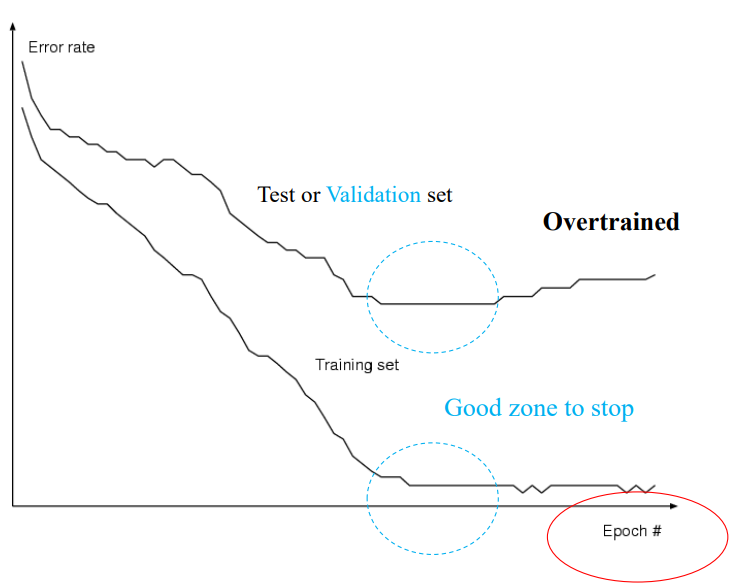
\includegraphics[scale=0.5]{8.png}
\end{center}
How to act on the overtraining?
\begin{list}{}{}
	\item \textbf{Early stopping}: using a validation set to determine when to stop (vague indication: when the validation error increases, so use more than one epoch before estimating (\textbf{patience}))\\
	Since the effective number of parameters grows during the training, halting the process effectively limits the complexity.
	\item \textbf{Regularization} on the loss: we can optimize the loss considering the weights values.\\
	Related to Tikhonov, so well principled approach: add a penalty term to the error function: $$\text{Loss}(\mathbf{w}) = \sum_p (d_p - f(\mathbf{x}_p))^2 \underline{+\lambda||\mathbf{w}||^2}$$ with $||\mathbf{w}||^2 = \sum_i w_i^2$\\
	The effect is a weight decay, basically $$\mathbf{w}_{new} = \mathbf{w} + \eta\cdot\Delta \mathbf{w} - 2\lambda \mathbf{w}$$
	$\lambda$ is the \textbf{regularization parameter}, generally very low (0.01) and selected in the model selection phase. Applied on the linear model it's the ridge regression.\\
	More sophisticated penalty terms have been developed (e.g.: weight elimination with Haykin).
	Misunderstandings:
	\begin{list}{}{}
		\item Regularization is not a technique to control the stability of the training convergence but controls the \textbf{complexity of the model}, measured by VC-dim and related to the number of weights and values of the weights in the neural networks
		\item Early stopping needs a validation set to decide when to stop, which sacrifices some data. The regularization is a principled approach, as it allows the VL curve to follow the TR curve so that early stopping is not needed.\\
		But you can use both!
	\end{list}
	Typically the bias ($w_0$) is omitted because its inclusion causes the results to be not independent from target shift/scaling. May be included with its own regularization coefficient.\\
	Typically it's applied in the batch version. So for online/mini batch we need to take into account possible effects over many steps, so it's better to use $\lambda\cdot\frac{mb}{l}$ with $l$ being the number of total patterns.\\
	Other techniques: \textbf{dropout}.
	\item \textbf{Pruning methods}
\end{list}
%TODO from here ML-21-NN-part2-v0.12.pdf p.59
\subparagraph{Number of units} This is related to the control of complexity but also to the input dimension and the size of the TR set. In general, this is a model selection issue. The number of units, along with the regularization parameters, can be selected with the model selection phase (cross-validation).\\
Too few units $\Rightarrow$ underfitting, viceversa too many units $\Rightarrow$ overfitting. The number can be high with proper regularization.
\begin{list}{}{}
	\item \textbf{Constructive approaches}: the learning algorithm decides the number of hidden units, starting with small networks and adding new units.\\
	Incremental approach: algorithms that build a network starting with a minimal configuration and add new units and connections during training. Examples: Tower, Tiling Upstart for classification and Cascade Correlation for both regression and classification.\begin{list}{}{}
		\item The \textbf{Cascade Correlation} algorithm starts with N0, a network without hidden units, which is trained and evaluated. If N0 cannot solve the problem, go to N1: a hidden unit is added such that the correlation between the output of the unit and the residual error of N0 is maximized (by training its weights).\\
		After training, the weights of the new unit are frozen and the remaining weights are restrained. If the obtained network N1 cannot solve the problem, new hidden units are progressively added, which are connected with all the inputs and previously installed units. The process continues until the residual errors of the output layer satisfy a specified stopping criteria.\\
		This method dynamically builds up a neural network and terminates once a sufficient amount of hidden units has been found to solve the given problem. Specifically, it works by interleaving the minimization of the total error function (LMS) by simple backpropagation training of the output layer and the maximization of the (non-normalized) correlation (the covariance) of the new inserted hidden (candidate) units with the residual error. With $E_{p,k} = (o_{p,k} - d_{p,k})$ residual error, with $o_{p,k}$ output, $p$ pattern and $k$ output unit
		$$S = \sum_k\:\vline\sum_p(o_p - mean_p(o_{p,k}))(E_{p,k} - mean_p(E_{p,k}))\vline$$
		$$\frac{\partial S}{\partial w_j} = \sum_k sign(S_k)\sum_p(E_{p,k} - mean_p(E_{p,k}))f'(net_{p,h})I_{p,j}\:\:\text{with }h\text{ candidate index}$$
		\begin{center}
			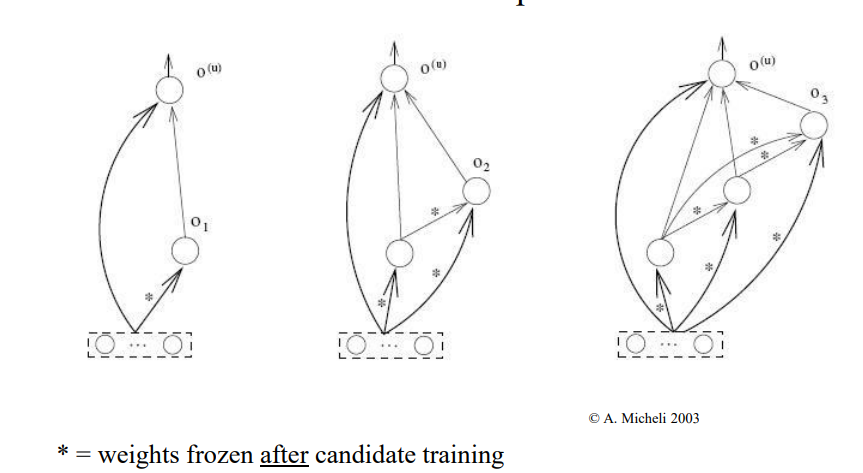
\includegraphics[scale=0.5]{9.png}
		\end{center}
		The role of hidden units is to reduce the residual output error (solves a specific sub-problem and becomes a permanent "feature detector").\\
		Typically, since the maximization of the correlation is obtained using a gradient descent technique on a surface with several maxima, a pool of hidden units is trained and the best one selected to avoid local maxima. It's also greedy: easy to converge may also find a minimal number of units but may lead to overfitting.
\end{list}
	\item \textbf{Pruning methods}: start with a large network and progressively delete weights or units.
\end{list}
\subparagraph{Input scaling and output representation} Preprocessing can have large effects: normalization (via standardization and rescaling), categorical inputs, handling missing data\ldots\\
For the output, one or more linear units for regression. For classification, one unit (binary classification) or one of $k$ (multioutput):
\begin{list}{}{}
	\item sigmoid (choose the threshold to assign to class)
	\item rejection zone
	\item one-of-$k$ encoding (winner class chosen by taking the highest value among the outputs)
	\item Often symmetric logistic (tanh) learn faster
	\item Softmax for 0/1 targets, sum to 1 can be interpreted as probability of belonging to class $i$ among $k$ classes.
\end{list}
\section{Model Selection and Model Assessment}
\subsection{Bias-Variance} A bias-variance decomposition provides an useful framework to understand the validation issue, showing how difficult is the estimation of a model's performance, again showing the need of a trade-off between fitting capabilities (\textbf{bias}) and model flexibility (\textbf{variance}).
\begin{center}
	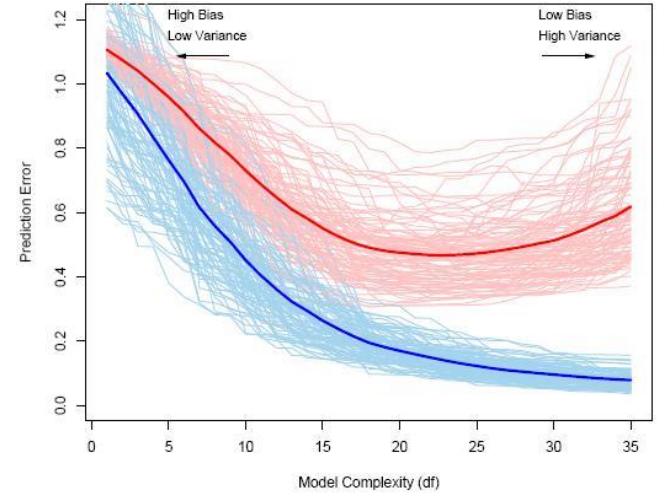
\includegraphics[scale=0.75]{10.png}
\end{center}
\subsection{Motivations} We are looking for the best solution, with minimal test error: looking for a balance between fitting (accuracy on training data) and model complexity. The \textbf{training error is not a good estimate of the test error}.\\
Assuming that we have a set of tuning parameters $\Theta$, implicit or explicit, that varies the model complexity, we wish to find the value of $\Theta$ that minimizes test error: \textbf{methods for estimating the expected error} for a model (or each model of a class of models, or event a set of models\ldots)
\subsection{Validation}
We can approximate the estimation analytically:
\begin{list}{}{}
	\item AIC, BIC, Bayesian Information Criterion (limited to linear models)
	\item MDL
	\item Structural Risk Minimization and VC-Dimension
\end{list}
In practice, we can approximate the estimation on the data set by resampling, a direct estimation of error via cross-validation (hold-out, K-fold\ldots), bootstrap\ldots
\paragraph{Two aims} \begin{list}{}{}
	\item \textbf{Model Selection}: estimating the performance of different learning models in order to choose the best one (to generalize), which includes looking for the best hyperparameters of the model.\\
	It \textbf{returns a model}.
	\item \textbf{Model Assessment}: after choosing the final model (or class of models), estimating/evaluating the generalization error on \textbf{new test data}.\\
	It \textbf{returns an estimation value}.
\end{list}
The gold rule is to keep a separation between goals and to use separate data sets: \textbf{hold out}, if data set is sufficient, for example 50\% TR, 25\% VL and 25\% TS (\textbf{disjoint sets!})
	\begin{center}
		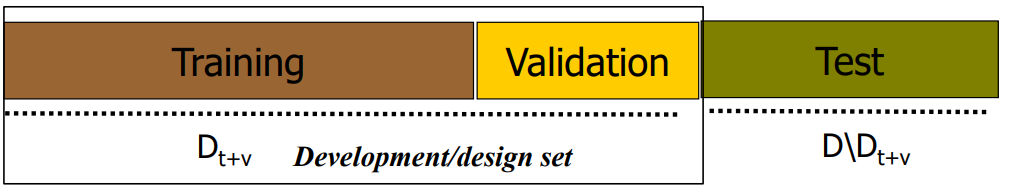
\includegraphics[scale=0.5]{11.png}
	\end{center}
The TR is the \textbf{training set}, VL is the \textbf{validation}/selection \textbf{set} (used to perform the \textbf{model selection}) and the TS is the \textbf{test set} (used for the model assessment).\\
If the test set is used repeatedly in the design cycle we would be doing model selection, and not reliable assessment. \textbf{Blind test set} concept: \textit{if you see the solution it's not a test}. In that case the test error would be an overoptimistic evaluation of the true test error. It's very easy to obtain very high classification accuracy over random tasks even when using the test set only implicitly.
\begin{center}
	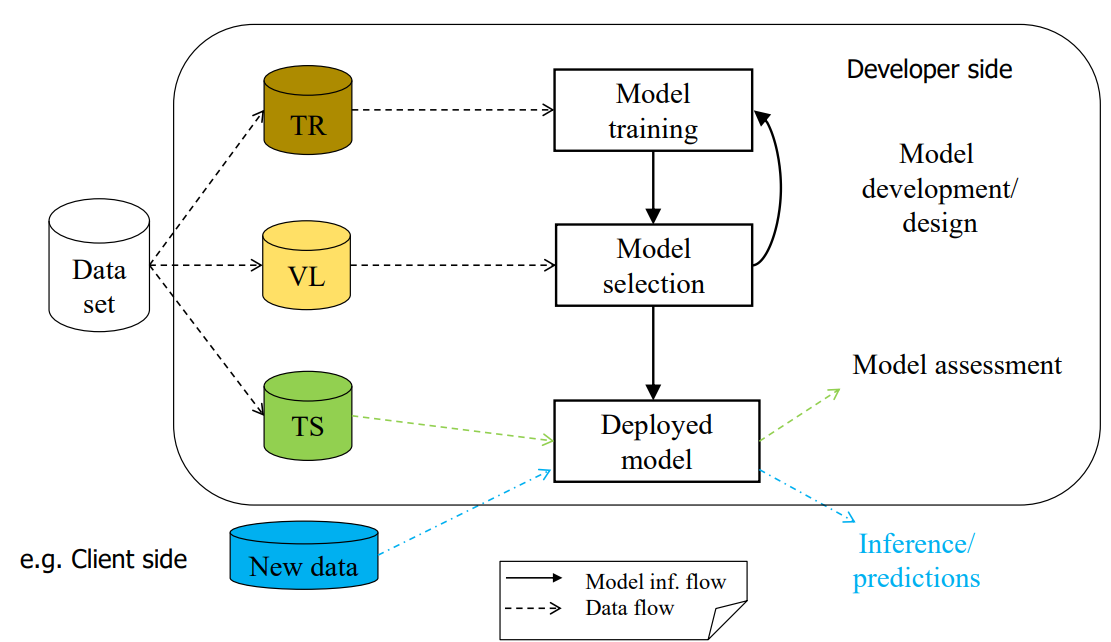
\includegraphics[scale=0.5]{12.png}
\end{center}
\paragraph{Grid Search} For the model selection: hyperparameters can be set by searching in a hyperparameters space. Try every hyperparameter-value combination and record the result. The best result will corresponds to the best hyperparameter values.\\
The cost can be high (cartesian product between sets of values per each hyperparameter: what if 6 hyperparameters each with tens of possible different values? So many combinations), so can be useful to fix some hyperparameter value before: more levels of grid search, where we do a first coarse grid search to find good intervals of values, then a finer grid-search can be performed over smaller intervals.
\paragraph{K-fold Cross Validation} Split the data set $D$ into $K$ mutually exclusive subsets $D_1,\ldots, D_k$, we train on $D - D_i$ and test it on $D_i$. No unique model, but we get a variance (std. dev.) over different folds for the class of models or algorithm.
\begin{center}
	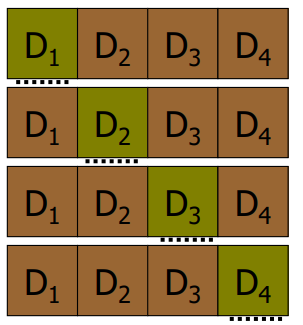
\includegraphics[scale=0.5]{3.png}
\end{center}
The issue is to find $K$ and that this method can be very computationally expensive but it can be combined with validation set,  double-K-Fold cross-validation\ldots
\paragraph{Double cross-validation} After dividing the data set into $K$ mutually exclusive subsets $D_1,\ldots, D_k$, for each $D_i$: do another \textbf{internal} cross-validation using the other $K-1$ subsets.
\begin{center}
	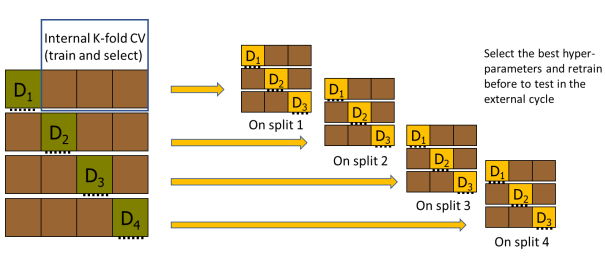
\includegraphics[scale=0.7]{13.png}
\end{center}
It doesn't provide a model but an estimation of the risk, because can provide a different model per external step cycle.
\paragraph{Example with K-Fold CV} Split data in TR and TS.\\
For the \textbf{model selection}, use K-Fold cross-validation over TR, obtaining new TR and VL in each fold, to find the best hyperparameters of the model.\\
\textbf{Train} the final model on the whole, original, TR.\\
Perform the \textbf{model assessment} by evaluating it on the external TS.\\\\
There are more combination and more ways of doing this.
\paragraph{Particular cases} 
\subparagraph{Lucky/unlucky sampling} Can we avoid to be sensible to the particular partitioning of the examples?
\begin{list}{}{}
	\item \textbf{Stratification}: the process of grouping examples into relatively homogeneous subgroups. For example, partitioning in a way that every class (in a classification task) is represented in approximately the same proportions as in the full data set.\\
	\item  \textbf{Repeated} hold-out or K-Fold CV: repeating the splitting with different random sampling, average the results to yield an overall estimation.
\end{list}
\subparagraph{Very few data} In this case it's difficult to say if the sampling is representative or not. We can use stratification.\\
To avoid (or to be considered during evaluation): missing classes or features in training data, special classes, known outliers that can affect the results\ldots\\
Also the blind test set can be misleading if: is from a different distribution, measured with a different scale/tolerance, uncleaned, unprocessed\ldots
\subparagraph{When to stop?} Best to avoid stopping the model training by fixing an arbitrary number of epochs: if it's too small it may be to early (underfitting), and too high may be too late (overfitting), may not old for all the configuration in a cross-validation\ldots\\
Also selecting the number of epochs by model selection it's not the best practice: better than a fixed number, but still not accurate.
\subparagraph{Early Stopping} Should be part of the model selection as well. Tricky: uses part of the data just to decide when to stop, also complex with cross-validation.\\
How to select the best model with early stopping for the final retraining (example: different stop points for each validation set in a cross-validation)? You could take the average number of epochs, but varying the data for retraining after model selection could lead to a different (better) stop point. So it's better to consider the average of the TR error at the best point and use it to gain the same level of fitting on the retraining. Else you need a VL every time you train.
\subparagraph{Random initialization} Different $w_{initial} \Rightarrow$ different models: how to chose one for the final model? You can compute the mean and variance of error/accuracy across the different trials, so that a random case would be in this range.
\section{Statistical Learning Theory}
\subsection{VC-dim} The VC-dim is used to provide the analytical bound we need to evaluate $H$. It's a measure of complexity (that is to say, capacity/expressive power/flexibility) of a class of hypothesis.\\
The bound is expressed not in terms of $|H|$ but in terms of distinct instances that can be completely discriminated using $H$. Intuitively (for classification): how much can $H$ discriminate points? The maximum number of points that can be correctly classified/learned without error for all the possible labelings.
\paragraph{Shattering} Given $X$ instance/input space, $n$ size of the instance space (number of instances) and $l$ for the number of data available. $H$ is the hypothesis space.\\
In the case of binary classification, there are $2^n$ possible \textbf{dichotomies} (partitions or labeling of the $n$ points in $\{-1,+1\}$): a particular dichotomy is represented in $H$ if there exists a hypothesis $h\in H$ that realizes the dichotomy.\\
\textbf{Definition}: $H$ shatters $X \Leftrightarrow H$ can represent all the possible dichotomies on $X$ (0 errors). The points in $X$ can be separated by an $h\in H$ in all the possible ways, and for every possible dichotomy of $X$ there exists a consistent hypothesis $h\in H$
\subparagraph{Example} \begin{multicols}{2}
\begin{center}
	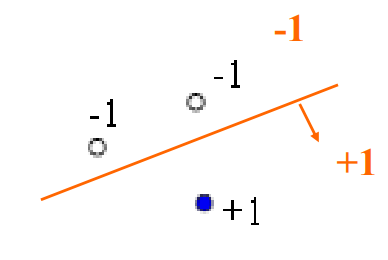
\includegraphics[scale=0.5]{14.png}
\end{center}
\columnbreak
3 points in $R^2$, $H$ as a set of lines: $h(x) = \text{sign}(wx + w_0)$ with $x\in \mathbb{R}^2$\\
A dichotomy is a particular labeling in $\{-1,+1\}$ of the points. This specific dichotomy can be represented in $H$: there exist a line that correctly separate the points (in pic)
\end{multicols}
\paragraph{VC-Dimension} \textbf{Definition}: the VC dimension of a class of functions $H$ is the maximum cardinality of a set (configuration) of points in $X$ that can be shattered by $H$.\\
$VC(H) = p \Rightarrow H$ shatters \textbf{at least one} set of $p$ points $\wedge$ $H$ \textbf{cannot shatter any} set of $p+1$ points.\\
If arbitrarily large but finite sets of $X$ can be shattered by $H$ then $VC(H) = \infty$\\\\
$VC(H)\geq 3$ shown before, note that not all the possible configurations of $3$ points can be shattered (example follows), but it's sufficient to find one configuration of three points which is separable for every labeling.
\begin{center}
	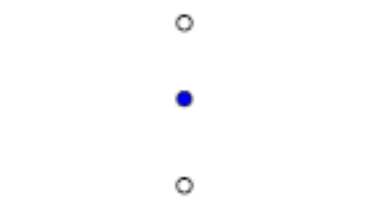
\includegraphics[scale=0.5]{15.png}
\end{center}
VC-dim is related to the number of parameters, but it's not the same thing: we may add redundant free parameters, for example, and there exists models with one parameter and infinite VC-dim. For example, $K$-NN has infinite VC-dim.
\paragraph{Analytical Bound} With $N$ number of data $$R[h]\leq R_{emp}[h] + \epsilon\left(\text{VC-dim}, N, \delta\right)$$
with:
\begin{list}{}{}
	\item \textbf{Guaranteeded risk} $R_{emp}[h] + \epsilon\left(\text{VC-dim}, N, \delta\right)$
	\item \textbf{VC Confidence} $\epsilon\left(\text{VC-dim}, N, \delta\right)$
\end{list}
For example, for 0/1 loss $$\epsilon\left(\text{VC-dim}, N, \delta\right) = \sqrt{\frac{VC\left(\ln\frac{2N}{\text{VC-dim}}\right) - \ln\frac{\delta}{4}}{N}}$$ with probability at least $1-\delta$ for every VC-dim$< N$\\\\
There are different bound formulations for different classes of functions, of tasks\ldots\\
This gives us a way to estimate the error on future data based only on the training error and the VC-dim of $H$. The resulting bounds are the worst case scenario, because the hold for all but $1-\delta$ of the possible approximation function/training sets.
\paragraph{Remarks} For many reasonable hypothesis classes (ex: linear approximators), the VC-dim is linear in the number of free parameters of the hypothesis. This shows that to learn "well" we need a number of examples that is linear in the VC-dim.
\subsection{Structural Risk Minimization} SRM uses VC-dim as a controlling parameter for minimizing the generalization bound on $R$. Assuming finite VC-dim, we can define a nested structure of models-hypothesis spaces according to the VC-dim in the following way:\begin{list}{}{}
	\item $H_1\subseteq H_2\subseteq \ldots\subseteq H_n$
	\item $VC(H_1)\leq VC(H_2)\leq \ldots\leq VC(H_n)$
\end{list}
Some examples:
\begin{list}{}{}
	\item Neural Networks with increasing number of hidden units, but also the number of epochs
	\item Polynomial of increasing degree
	\item Increasing values for $c$, in $||w||<c$ for regularization
	\item Increasing number of nodes in a decision tree
\end{list}
\paragraph{Model selection} Growing VC-dim: empirical (training) error decreasing, VC confidence increasing.\\
SRM: find a trade-off in the bound and choose the model ($h$) with the best bound on the true risk.
\begin{center}
	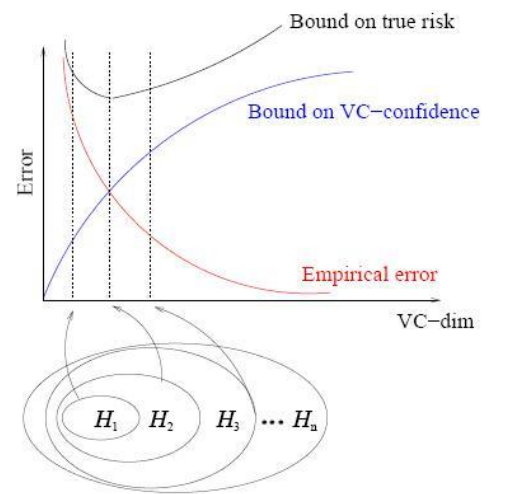
\includegraphics[scale=0.5]{16.png}
\end{center}
\paragraph{Use of the bound} Provide a fundamental theoretical ground for principled Machine Learning: independently from specific model details or learning algorithms, highlighting the role of complexity control. The optimal choice of the model complexity (structure) provides the minimum expected risk (\textbf{inductive principle of SRM})\\
Also used to provide a direction for new model development guided by SRM. As estimation of predictive errors is rarely used: the upper bound is overly pessimistic and may not be adequate for reliable evaluation of the generalization error (model assessment) and tighter bounds are under development, also is difficult to compute the VC-dim for specific classes of $H$.\\
Towards \textbf{principled approaches} less based on trial and error. For example, two practical approaches:
\begin{list}{}{}
	\item Choose appropriate structure/complexity, fix the model (hence the VC-dim) and minimize the TR error.\\
	Can be used in neural networks, however regularization by training heuristic can further introduce implicit SRM (early stopping\ldots) or SRM with Tikhonov regularization where we have minimum loss with $R_{emp} +$ complexity term, considering both the terms.
	\item Fix the TR error, automatically minimize the VC confidence (SVM)
\end{list}
\section{Support Vector Machines}
Linear machine, with maximization of the separation margin and structural risk minimization. Initially \textbf{hard margin SVM}, we assume to deal with linearly separable problems without errors in the data.\\
Example of linearly and non linearly separable problems:
\begin{center}
	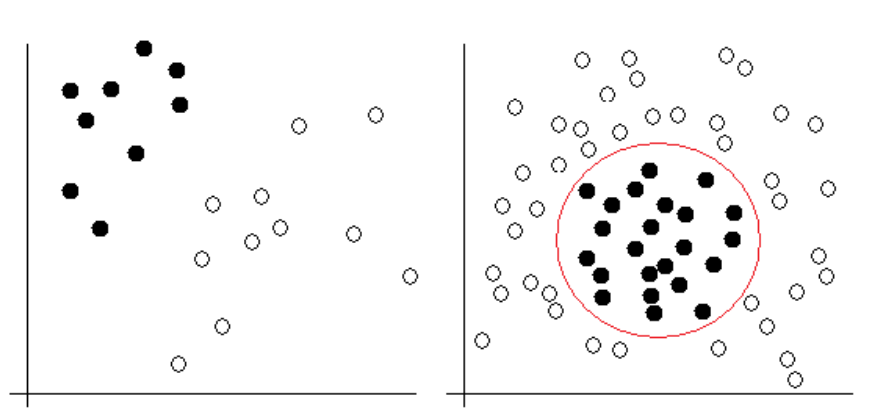
\includegraphics[scale=0.5]{17.png}
\end{center}
\paragraph{Separating hyperplane} Given the training set $T = \{(x_i, d_i)\}_{i=1}^N$ we want to find an hyperplane of equation $w^Tx + b = 0$ to separate the examples and get $w^Tx_i + b \geq 0$ for $d_i = +1$ and $w^Tx_i + b < 0$ for $d_i = -1$\\
$g(x) = w^Tx + b$ is the discriminant function and $h(x) = \text{sign}(g(x))$ is the hypothesis.\\
An example of separation margin:
\begin{center}
	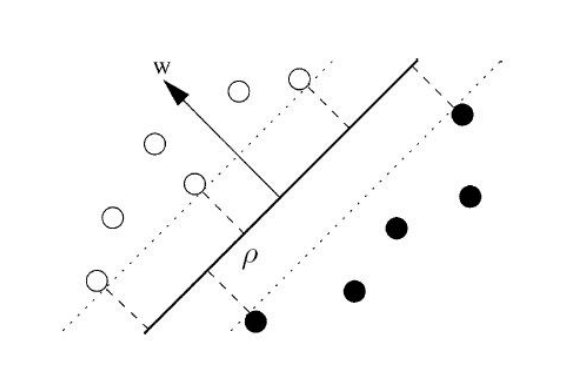
\includegraphics[scale=0.5]{18.png}
\end{center}
In this case the hyperplane has equal distance to both the closest negative and positive examples. The separation margin ($p$) is evaluated as the double of the distance between the linear hyperplane and the closest data point (a "safe zone"). Not all hyperplanes solving the task are equal: the margin changes, bigger or smaller. The \textbf{optimal hyperplane is the hyperplane which maximizes $p$} $w_O^Tx + b_O = 0$ with $_O$ meaning "optimal".\\
We will find that $p = \frac{2}{||w||}$, so maximize $p\Leftrightarrow$ minimize $||w||$.
\paragraph{Support Vector} We can rescale $w$ and $b$ so that the closest points to the separating hyperplane statisfy $|g(x_i)| = |w^Tx_i + b| = 1$, so we can write $$w^Tx_i + b \geq 1\text{ if }d_i = +1$$ $$w^Tx_i + b < 1\text{ if }d_i = -1$$ which its compact form is $$d_i(w^Tx_i + b) \geq 1\:\:\forall\:i=1,\ldots,N$$
A \textbf{support vector} $x^{(s)}$ satisfies the previous equation exactly $$d^{(s)}(w^Tx^{(s)}+b) = 1$$ so the \textbf{support vectors are the closest data points to the hyperplane} and "lay on the margin".
\begin{center}
	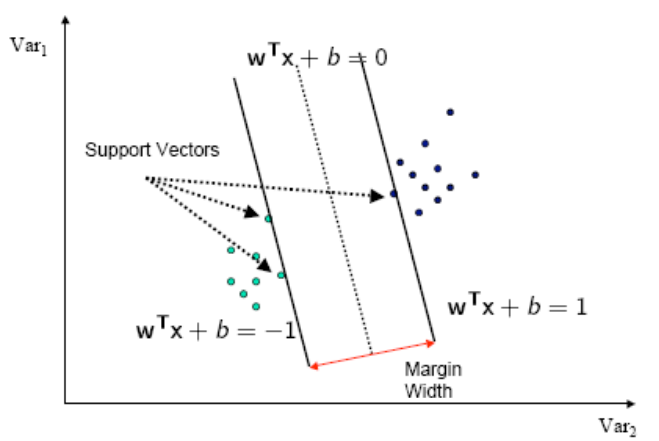
\includegraphics[scale=0.5]{19.png}
\end{center}
\paragraph{Computing the distance} With the discriminant function $g(x) = w^Tx + b$, recalling that $w_O$ is a vector orthogonal to the hyperplane. Let's denote with $r$ the distance between $x$ and the optimal hyperplane.
\begin{center}
	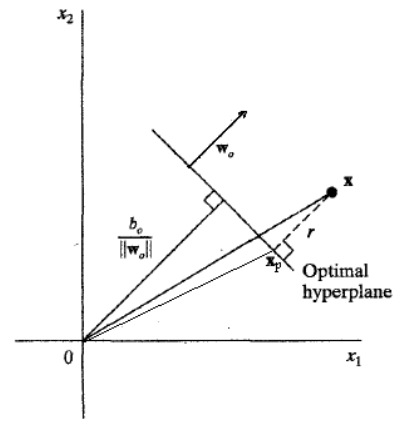
\includegraphics[scale=0.5]{20.png}
\end{center}
$$x=x_p+r\frac{w_O}{||w_O||}$$
$$g(x) = g\left(x_p + r\frac{w_O}{||w_O||}\right) ) w_O^Tx_o + b_O + w_O^Tr\frac{w_O}{||w_O||} = g(x_p) + rw_O^T\frac{w_O}{||w_O||} = r\frac{||w_O||^2}{||w_O||} = r||w_O||$$
$$\text{thus }r=\frac{g(x)}{||w_O||}$$
\paragraph{Computing the margin} Consider the distance between the hyperplane and a positive support vector $x^{(s)}$, for example $$r\text{ for }x^{(s)} = \frac{g(x^{(s)})}{||w_O||} = \frac{1}{||w_O||} = \frac{p}{2}$$
$$\Rightarrow p = \frac{2}{||w_O||}$$
So the optimum hyperplane maximizes $p\Leftrightarrow$ minimizes $||w||$
\paragraph{Quadratic Optimization Problem} The formal derivation of the SVM solution requires techniques in the constrained optimization framework, and we assume that quadratic programming is solved elsewhere.\\
For the hard margin SVM, the quadratic optimization problem asks to find the optimum values of $w$ and $b$ in order to maximize the margin.
\subparagraph{Primal Form} Given the training examples $T = \{(x_i, d_i)\}_{i=1}^N$, find the optimum values of $w$ and $b$ which minimizes $$\psi(w) = \frac{1}{2}w^Tw$$ satisfying the constraints $$d_i(w^Tx_i+b)\geq 1\:\:\:\forall\:i=1,\ldots,N$$
The objective function $\psi(w)$ is quadratic and convex in $w$, while the constraints are linear in $w$: solving this problem scales (the computational cost) with the size of the input space $m$.\\
The Lagrangian multipliers method is used: constructing the Lagrangian function corresponding to the quadratic optimization problem $$J(w, b,\alpha) = \frac{1}{2} w^Tw - \sum_{i=1}^N\alpha_i\left(d_i\left(w^Tx_i+b\right)-1\right)$$ with $\alpha_i \geq 0$ the $N$ Lagrangian multipliers. Each term in the sum correspond to a constraint in the primal problem. $J$ must be minimized with respect to $w$ and $b$, and maximized with respect to $\alpha$, and the solution correspond to a saddle point in $J$.\\\\
We will find $$w_O = \sum_{i=1}^N \alpha_{O,i}d_ix_i$$ thus the optimal hyperplane is expressed as $$w^T_Ox+b_O = 0 \Leftrightarrow \sum_{i=1}^N\alpha_{O,i}d_ix_i^Tx + b_O = 0$$
The optimal conditions will be:
\begin{list}{}{}
	\item Minimize $J$ with respect to $w \Rightarrow\frac{\partial J}{\partial w} = 0 \Rightarrow w = \sum_{i=1}^N \alpha_id_ix_i$
	\item Minimize $J$ with respect to $b \Rightarrow\frac{\partial J}{\partial b} = 0 \Rightarrow w = \sum_{i=1}^N \alpha_id_i$
\end{list}
And we may substitute these in $J$ to study the dual form.
\subparagraph{Kuhn-Tucker Conditions} From the KT conditions follows that $$\alpha_i(d_i(w^Tx_i + b) - 1) = 0\:\:\:\:\forall\:i=1,\ldots, N$$ in the saddle point of $J$:
\begin{list}{}{}
	\item $\alpha_i > 0 \Rightarrow d_i(w^Tx_i+b) = 1$ and $x_i$ is a support vector
	\item $x_i$ isn't a support vector $\Rightarrow \alpha_i = 0$
\end{list}
Hence we can restrict the computation to $N_s$ so $w_O=\sum_{i=1}^{N_s} \alpha_{O,i}d_ix_i$: \textbf{the hyperplane depends solely on the support vectors}!\\\\
To obtain the Lagrangian multipliers $\{a_i\}_{i=1}^N$ we must solve the dual form: given the training examples $T = \{(x_i, d_i)\}_{i=1}^N$, find the optimum values of $\{a_i\}_{i=1}^N$ that maximizes $$Q(\alpha) = \sum_{i=1}^N \alpha_i - \frac{1}{2}\sum_{i=1}^N\sum_{j=1}^N\alpha_i\alpha_jd_id_jx_i^Tx_j$$ satisfying the constraints $$\alpha_i\geq 0\:\:\:\forall\:i=1,\ldots,N$$ $$\sum_{i=1}^N\alpha_id_i = 0$$
Then we compute $w_O = \sum_{i=1}^N\alpha_{O,i}d_ix_i$ and $b_O = 1-w_O^Tx^{(s)}$ corresponding to a positive support vector $x^{(s)}$, so $$b_O = = 1-\sum_{i=1}^N\alpha_{O,i}d_ix_i^Tx^{(s)}$$
So we don't need to explicitly compute $w_O$, but we only need the Lagrangian multipliers $\alpha_i$ (by solving the dual problem), then we compute the optimal bias $b_O$. The decision surface is given by $$w_O^Tx + b_O = 0 \Leftrightarrow\sum_{i=1}^N\alpha_{O,i}d_i x_i^Tx + b_O = 0$$
So given the input pattern $x$:
\begin{list}{}{}
	\item Compute $g(x) = \sum_{i=1}^N \alpha_{O,i}d_ix_i^Tx + b_O$
	\item Classify $x$ as the sign of $g(x)$
\end{list}
Note that it's not necessary to compute $w_O$, also the sum can be restricted to the number of support vector $N_s$
\subparagraph{How does this improve the generalization?} Minimizing the norm of $w$ is equivalent to minimizing the VC-dim and thus to minimizing the VC confidence $\epsilon$ in $$R[h] \leq R_{emp}[h] + \epsilon(\text{VC-dim}, N, \delta)$$
\subparagraph{Theorem (Vapnik)} Let $D$ be the diameter of the smallest ball around the data points $x_1,\ldots,x_N$. For the class of separating hyperplanes described by the equation $w^Tx+b = 0$, the upper bound to the VC-dim is $$\text{VC-dim} \leq min(\lceil\frac{D^2}{p^2}\rceil, m_O) + 1$$
\paragraph{An elegant approach} For linearly separable data there are many solutions. Vapnik proposed an "optimal separating hyperplane" maximizing the margin providing:
\begin{list}{}{}
	\item An unique solution with zero errors for the binary classifier
	\item An automatized approach to SRM that minimizes VC confidence (by maximizing the margin) as part of the training process, without hyper parameters in the linear separable case.
	\item The use of a solver in the class of constrained quadratic programming (instead of gradient descent) with a dual form (showing support vectors and dot product among the patterns)
	\item A solution focused on "selected" training data (support vectors)
\end{list}
For noisy or not linearly separable data, you can have a soft margin (support vector still on the border, but some data may fall closer to the hyperplane: at least one point violate $d_i(w^Tx_i+b)\geq 1$)
\paragraph{Soft margin SVM} We introduce $\xi_i\geq 0\:\:\:\forall\:i=1,\ldots, N$ called \textbf{slack variables}: $d_i(w^Tx_i+b)\geq 1-\xi_i$, so a support vector satisfies that exactly $d_i(w^Tx_i+b)\geq 1-\xi_i$
\begin{center}
	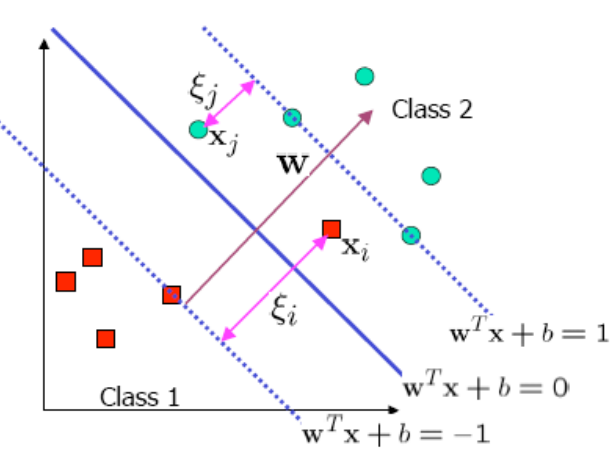
\includegraphics[scale=0.5]{21.png}
\end{center}
Note that Vapnik does not hold anymore. The primal problems becomes: given the training examples $T = \{(x_i, d_i)\}_{i=1}^N$, find the optimum values of $w$ and $b$ which minimizes $$\psi(w, \xi) = \frac{1}{2}w^Tw + C\sum_{i=1}^N\xi_i$$ satisfying the constraints $$d_i(w^Tx_i+b)\geq 1\:\:\:\forall\:i=1,\ldots,N$$ $$\xi_i\geq 0\:\:\:\forall\:i=1,	\ldots, N$$
We introduced $C$ as a regularization hyperparameter, losing the fully automated SRM. Low $C$ means many TR errors allowed (possible underfitting), while high $C$ means less or no TR errors allowed (smaller margin, possible overfitting)
\subparagraph{Kuhn-Tucker Conditions} The KT conditions are now defined as
\begin{list}{}{}
	\item $\forall\:i=1,\ldots,N\:\:\:\alpha_i(d_i(w^Tx_i + b)+\xi_i - 1) = 0$
	\item $\forall\:i=1,\ldots,N\:\:\:\mu_i\xi_i=0$ with $\mu_i$ Lagrangian multipliers introduced to enforce the non negativity of the slack variables.
\end{list}
We have $0<\alpha_i<C\Rightarrow\xi_i = 0$ on the margin and $\alpha_i=C\Rightarrow\xi_i > 0$ inside the margin.
\subparagraph{Solving the problem} We solve the dual problem to compute the $\{\alpha_i\}_{i=1}^N$, then we find $w_O$ and $b_O$ from $\{\alpha_{O,i}\}_{i=1}^N$ with $w_O = \sum_{i=1}^N\alpha_{O,i}d_ix_i$\\
Then, for a pattern $j$ such that $0<\alpha_j<C$, we have $$b_O = d_j-\sum_{i=1}^N\alpha_{O,i}d_ix_i^Tx_j$$
or an average of all the solutions for numerical stability. The non-zero Lagrangian multipliers correspond the the support vectors. We use it as before: $g(x) = \sum_{i=1}^N \alpha_{O,i}d_ix_iTx + b_O$ and $h(x) = sign(g(x))$
\subsection{High-Dimensional feature spaces} We can use:
\begin{list}{}{}
	\item Non-linear mapping of input patterns to a high-dimensional feature space\\
	\textbf{Cover's Theorem}: the patterns are linearly separable with high probability in the feature space under such conditions.
	\item Finding the optimal hyperplane to separate the patterns in the feature space.
\end{list}
However we know that using high dimensional feature spaces (large basis function expansion) can be computationally unfeasible and can lead to overfitting.\\
We will propose the kernel approach to implicitly manage the feature space while regularizing.
\paragraph{Kernel} Non linear function mapping $$\phi:R^{m_0}\rightarrow R^{m_1}$$ $$x\mapsto \phi(x)$$
The problem is formulated as before, but the training set is now $\{(\phi(x_i), d_i)\}_{i=1}^N$ and the hyper plane is now $w^T\phi(x) + b = 0$\\
The weight vector is a linear combination of the feature vectors
$$w=\sum_{i=1}^N\alpha_id_i\phi(x_i)$$ so the hyperplane equation is $$\sum_{i=1}^N\alpha_id_i\phi(x_i)^T\phi(x) = 0$$
Evaluating $\phi(x)$ could be intractable, but with certain conditions we don't need to evaluate it directly. We do not even need to know the feature space itself! This is possible using a function to compute directly the dot products in the feature spaces $k:R^{m_0}\times R^{m_0}\rightarrow R$, with $k$ called inner product kernel function: $k(x_i, x) = \phi(x_i)^T\phi(x)$, and it's symmetric meaning $k(x_i, x) = k(x, x_i)$\\
\subparagraph{Kernel Matrix} We can arrange the dot products in the feature space between the images of the input training patterns in a $N\times N$ matrix called kernel matrix $K = \{k(x_i, x_j)\}_{i,j=1}^N$, symmetrical.
\subparagraph{Mercer's Theorem} This property holds only for kernels with positive semi-definite kernel matrices. It's related to having non-negative eigenvalues in the kernel matrix.
\subparagraph{Properties} With $k_1,k_2$ kernels over $R^{m_0}\rightarrow R^{m_0}$, the following are also kernel functions:
\begin{list}{}{}
	\item $k_1(x,y)+k_2(x,y)$
	\item $\alpha k_1(x,y)$ with $\alpha\in \mathbb{R}^+$
	\item $k_1(x,y)\cdot k_2(x,y)$
\end{list}
\paragraph{Wrapping up}
\begin{list}{}{}
	\item The training set is $T = \{(x_i,d_i)\}_{i=1}^N$
	\item We can choose the trade-off parameter $C$ and the kernel function $k$
	\item We find $\{\alpha_i\}_{i=1}^N$ by solving the optimization problem via quadratic programming algorithms\\
	Remember that the solution is spars, as every $\alpha_i$ corresponding to non-support vector is $0$
	\item The bias $b_O$ is computed knowing the Lagrangian multipliers and the kernel matrix
	\item Given an input pattern $x$ we compute $w^T\phi(x) = \sum_{i=1}^N\alpha_id_ik(x,x_i)$\\
	Fundamental: we don't need to compute $w$
	\item $x$ is classified as $sign(g(x)) = sign\left(\sum_{i=1}^N\alpha_id_ik(x,x_i)\right)$ with $g(x)$ called discriminant function
\end{list}
At \textbf{test phase} we have the Lagrangian multipliers and the kernel matrix. To classify an unseen input pattern $x$, we compute $\sum_{i=1}^N\alpha_id_ik(x,x_i)$ and classify $x$ and the sign of that computation, so $h(x) = sign\left(\sum_{i=1}^N\alpha_id_ik(x,x_i)\right)$
\paragraph{Examples of kernels}
\begin{list}{}{}
	\item \textbf{Polynomial Learning Machine} $k(x,x_i) = (x^Tx_i + 1)^p$ with $p$ user-specified parameter
	\item \textbf{Radial Basis Function} or \textbf{Gaussian Kernel} $k(x,x_i) = e^{-\frac{1}{2\sigma^2}||x-x_i||^2}$ with $\sigma^2$ user-specified parameter.\\
	Narrow peaked kernels with small $\sigma$, imply that the reply for $x_i$ is only $d_i$\\
	Feature space with an infinite number of dimensions
	\item \textbf{Two-layer perceptron} $k(x,x_i) = tanh(\beta_0x^Tx_i + \beta_1)$ where $\beta_0 > 0$ and $\beta_1 < 0$ are user-specified parameters\\
	Here the Mercer's Theorem holds only for some choices of $\beta_0,\beta_1$
\end{list}
\subsection{SVM for non-linear regression}
A regression problem requires to find $f$ such that $d=f(x)+v$ with a training set $T=\{(x_i,d_i)\}_{i=1}^N$ and with $v$ statistically independent from $x$\\
We estimate $d$ using a linear expansion of non-linear functions $\{\phi_j(x)\}_{j=0}^{m_1}$ so $y=h(x) = w^T\phi(x)$ where $w = (w_0 = b, w_1,\ldots,w_{m_1})^T$ and $\phi(x) = (\phi(x)_0 = 1, \phi(x)_1,\ldots, \phi(x)_{m_1})^T$
\paragraph{$\epsilon$-insensitive loss function} $L_\epsilon(d,y) = \left\{\begin{array}{l l}
|d - y| - \epsilon & \text{if }|d-y|\geq\epsilon\\
0 & \text{otherwhise}
\end{array} \right.$
\begin{center}
	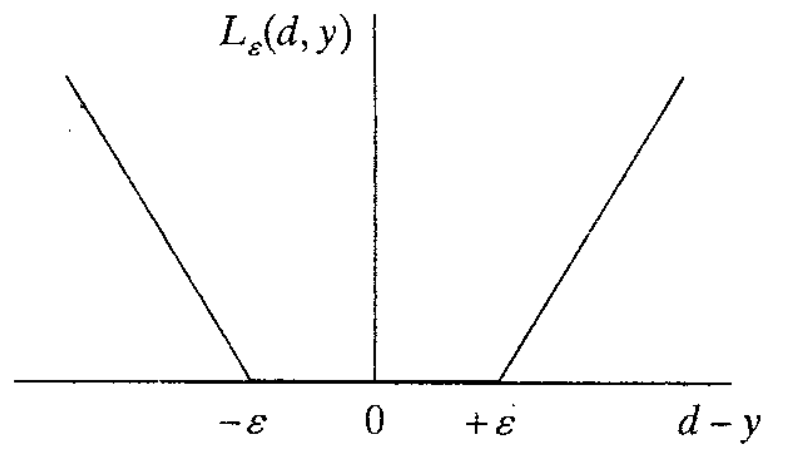
\includegraphics[scale=0.5]{22.png}
\end{center}
\paragraph{Optimization problem} Introducing the non-negative slack variables $\xi_i'$ and $\xi_i\forall\:i=1,\ldots,N$ $$-\xi_i'-\epsilon \leq d_i-w^T\phi(x_i)\leq \epsilon + \xi_i$$
leading to the following constraints, all $\forall\:i=1,\ldots,N$
\begin{list}{}{}
	\item $d_i - w^T\phi(x_i)\leq \epsilon + \xi_i$
	\item $w^T\phi(x_i)-d_i\leq \epsilon + \xi_i'$
	\item $\xi_i\geq 0$
	\item $\xi_i'\geq 0$
\end{list}
The primal problem then is: given the training set $\{(x_i, d_i)\}_{i=1}^N$ find the optimal values of $w$ such that the following objective function is minimized $$\psi(w,\xi,\xi') = \frac{1}{2}w^Tw + C\sum_{i=1}^N\left(\xi_i+\xi_i'\right)$$ under the constraints, all $\forall\:i=1,\ldots,N$
\begin{list}{}{}
	\item $d_i - w^T\phi(x_i)\leq \epsilon + \xi_i$
	\item $w^T\phi(x_i)-d_i\leq \epsilon + \xi_i'$
	\item $\xi_i\geq 0$
	\item $\xi_i'\geq 0$
\end{list}
The dual problem yields the optimal $\{\alpha_i\}_{i=1}^N$ and $\{\alpha_i'\}_{i=1}^N$. With those, we can compute the optimal $w$ $$w=\sum_{i=1}^N(\alpha_i - \alpha_i')\phi(x_i) = \sum_{i=1}^N\gamma_i\phi(x_i)$$
with $\gamma_i = \alpha_i - \alpha_i'$: in this case support vectors correspond to non-zero values of $\gamma_i$\\
The estimate is defined as $h(x) = y = w^T\phi(x)$, and using the linear expansion for $w$ we get $$h(x) = \sum_{i=1}^N\gamma_i\phi(x_i)^T\phi(x) = \sum_{i=1}^N\gamma_i k(x_i, x)$$
\paragraph{Wrapping up}
\begin{list}{}{}
	\item \textbf{Important}: select values for the user-specified parameters $C$ and $\epsilon$
	\item \textbf{Important}: choose an inner product kernel function $k$
	\item Compute the kernel matrix $K$
	\item Solve the dual form and get the optimal values of the Lagrangian multipliers ($\{\gamma_i\}_{i=1}^N$)
	\item Compute the optimal value for the bias ($b$)
	\item Obtain the estimate function as a linear combination of dot products in a feature space we can ignore ($h(x) = \sum_{i=1}^N \gamma_ik(x_i, x)$)
\end{list}
The test: given an input pattern $x$, we estimate the value of the unknown function $f$ in that point using the estimate computed before $$h(x) = \sum_{i=1}^N\gamma_i k(x_i,x)$$
\paragraph{Summary of the main characteristics}
\subparagraph{Pros}
\begin{list}{}{}
	\item The regularization is embedded in the optimization problem (margin)
	\item Approximation of the theoretical structure risk minimization
	\item Convex problem (\textbf{training always finds a global minimum})
	\item Implicit feature transformation using kernels
\end{list}
\subparagraph{Cons}
\begin{list}{}{}
	\item Must choose the kernel and its parameters
	\item It's a batch algorithm
	\item Very large problems are computationally intractable\\
	Problems with more than 20000 examples are very difficult to solve with standard approaches. However many solution are proposed (including gradient descent approaches)
\end{list}
\subparagraph{In practice} There is no theory which guarantees that a given family of SVMs will have high accuracy on a given problem.\\
The nice property of hard-margin SVMs cannot be directly extended to soft-margin and kernels: the $C$ parameter and kernels can lead to infinite VC-dim of the SVM classifier.\\
Gaussian RBF SVMs of sufficiently small width can classify an arbitrarily large number of training points correctly (only 1 SV point, the closest one, will contribute to the solution), thus have infinite VC-dim. On the opposite, with large width of the gaussian all SV points are considered and you get a sort of "global average", low VC-dim.\\
$\Rightarrow$ controlling the width is controlling the VC-dim.\\\\
Rigorous selection of the kernel and the $C$ requires an estimation of the complexity (VC-dim). Hyperparameters affecting model complexity are used for model selection. In practice a careful empirical evaluation.\\\\
Nowadays, deep neural networks have largely outperformed previous records of SVMs on image and speech recognition tasks.
\subsection{Kernel Methods}
The kernel trick introduces the kernel methods, also without SVM. \textbf{Kernelization} of previous approaches, whenever you had a dot product inside your model or a similar measure enabling them to operate in a new implicit high-dimensional space just by specifying a kernel (and changing it: \textbf{the $K$ can change without changing the learning machine}.
\begin{center}
	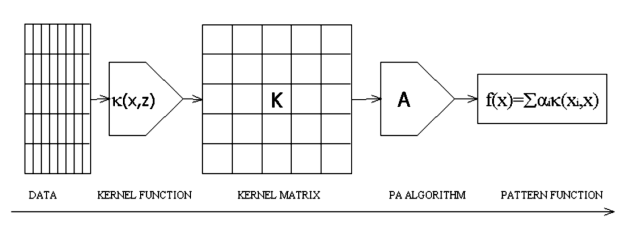
\includegraphics[scale=0.75]{23.png}
\end{center}
An SVM is largely characterized by the kernel: the best choice of kernel for a given problem is still a research issue.
\section{Bias-Variance} A training set is only one possible realizations from the universe of the data: different TR sets can provide different estimate. The expected error (on various TR) at a point $x$ is decomposed as:
\begin{list}{}{}
	\item \textbf{Bias}: quantifies the discrepancy between true function and $h(x)$ (averaged on data)
	\item \textbf{Variance}: quantifies the variability of the response of the model $h$ for different realizations of the TR data
	\item \textbf{Noise}: error in the label
\end{list}
Let's assume the regression scenario with target $y$ and L2 squared error loss. Suppose we have examples $(x,y)$ where the true function is $y = f(x) + \epsilon$ with $\epsilon$ being Gaussian noise with 0 mean and $\sigma$ standard deviation. In linear regression, given a set of examples $(x_i,y_i)$ with $i = 1,\ldots,l$, we fit a linear hypothesis $h(x) = wx + w_0$ to minimize sum of the squared error over the training data $\sum_{i=1}^l (y_i - h(x_i))^2$\\
Because of the hypothesis class that we chose for some function $f$ (linear hypothesis), we have a \textbf{systematic prediction error}. Depending on the dataset that we have, the parameters $w$ that we find will be different.\\\\
Given a new data point $x$, what is the expected prediction error? Assume that the data points are drawn independently and identically distributed from a unique underlying probability distribution $P$. The goal is to compute, for an arbitrary new point $x$, $E_P[(y - h(x))^2]$ noting that there's a different $h$ and $y$ for each different "extracted" training set. $y$ is the value for $x$ that could be present in a data set, and the expectation is over \textbf{all training sets} that are drawn according to $P$. We will decompose this expectation into three components: bias, variance and noise.
\subparagraph{Recall of statistics} With $Z$ random variable of possible values $z_i$ with $i=1,\ldots,l$ and probability distribution $P(Z)$
\begin{list}{}{}
	\item \textbf{Expected value} or \textbf{mean} of $Z$ is $$\overline{Z} = E_P[Z] = \sum_{i=1}^l z_i\cdot P(z_i)$$ with the sum replaced by an integral and the distribution by a density function if $Z$ is continuous.
	\item \textbf{Variance} of $Z$ is $$Var[Z] = E[(Z - E[Z])^2] = E[Z^2] - E[Z]^2$$ with $$E[Z^2] = E[Z]^2 + Var(Z)$$
\end{list}
\subsection{Bias-Variance Decomposition}
$$E_P[(y - h(x))^2] = E_P[h(x)^2 - 2yh(x) + y^2] = E_P[h(x)^2] + E_P[y^2] - 2E_P[y]E_P[h(x)]$$
Let $\overline{h}(x) = E_P[h(x)]$ denote the \textbf{mean prediction} of the hypothesis at $x$ when $h$ is trained with data drawn from $P$. By doing some calculations, we obtain $\begin{array}{r c l l}
E_P[(y-h(x))^2] & = & E_P[(h(x) - E_P[h(x)])^2] + & \text{variance}\\
 & & (E_P[h(x)] - f(x))^2 + & \text{bias}^2 \\
 & & E_P[(y - f(x))^2] & \text{noise}^2
\end{array}$\\
So expected error is Variance + Bias$^2$ + Noise$^2$\begin{list}{}{}
	\item \textbf{Bias}: quantifies the discrepancy between true function and $h(x)$, with $h(x)$ averaged over different TR data (\textbf{systematic error})\\E.g. due to too small $H$, too rigid model.
	\item \textbf{Variance}: quantifies the variability of the response of model $h$ for different realizations of the training data.\\Due to too high flexibility
	\item \textbf{Noise}: event the optimal solution can be wrong.\\E.g. if for a give n$x$ there are more than one possible $d$.\\
	It's irreducible, doesn't depend on the model.
\end{list}
\begin{center}
	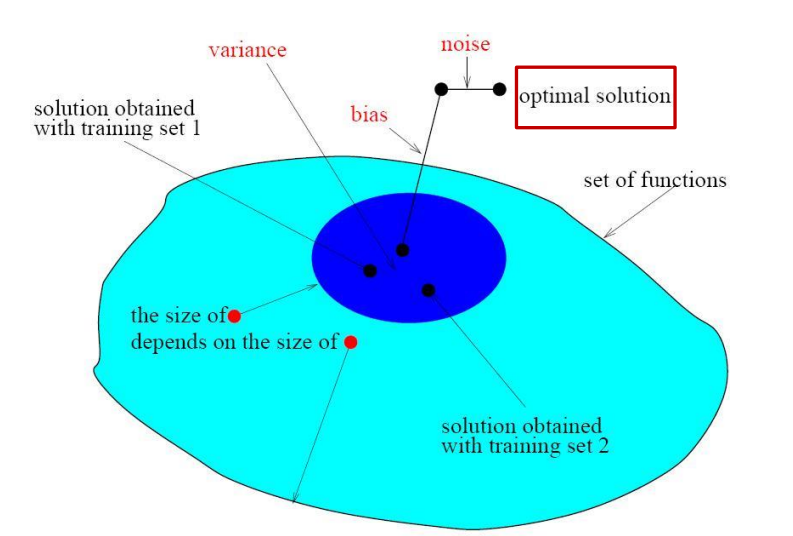
\includegraphics[scale=0.5]{24.png}
\end{center}
\section{Ensemble Learning}
\begin{center}
	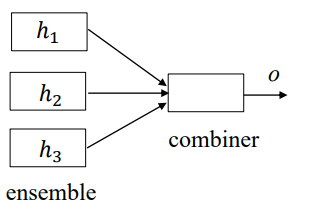
\includegraphics[scale=0.5]{25.png}
\end{center}
Take advantage of multiple models. In regression: simple average committee, mean square error of a committee\ldots In classification, take a vote over many classifier.
\subsection{Bagging} \paragraph{Bootstrap Aggregating} Combine many classifiers. Train $n$ classifiers on different subsets of TR and differentiate each training using bootstrap (resampling with replacement). Thing to bias-variance: high variance model can perform well on average. In other therms: the average of $h$ reduce the variance. In regression use the mean, in classification use the vote of the $n$ classifiers.
\subsection{Boosting} If the models have the same errors we have no advantage on esembling.\\
Differentiate each training concentrating on errors (more weight to difficult instances, e.g. more likely to be included in the TR of the next classifier, for example: train the 1st classifier, then train the 2nd with more weight on the instances misclassified before\ldots\\
Combine the results by output weights (weighted vote for classifiers, with more weight to low error classifiers).\\
If not stopped, boosting will learn to classify correctly all instances from TR, providing an incremental approach to construct complex models. Can suffer from noisy data (which are weighted more)
\subsection{Feature Selection} Find a selection of features that are more informative for the problem at hands. Benefits for: dimensionality reduction and filtering of irrelevant information and noise, interpretability\ldots\\
Computationally hard (many possible subsets of features, retraining\ldots) typically an heuristic search of the best subset by greedy or other optimization techniques.
\section{Applications} A huge number of successful applications in all the fields of ML.
\subsection{Character recognition (classification)}
\paragraph{First approaches} Standard NN with 256 inputs (16$\times$16 pixels): misclassification rate of 5/20\% (mostly due to lack of invariance as rotations ecc.)
\paragraph{Basic idea} Exploiting the architecture design to include pior information into NN:
\begin{list}{}{}
	\item Restricting the network architecture by extracting local features
	\item Constraining weights by sharing them among different units, as to reduce the number of free parameters while still allowing more complex connectivity (same operation on different part of the input, because the features of the characters should appear in different areas of the image
\end{list}
$\Rightarrow$ \textbf{Convolutional neural networks}
\subsection{Convolutional Neural Networks}
\paragraph{The name} Takes inspiration from the convolutional operator $$(f * g)(t) = \int_{-\infty}^\infty f(\tau)g(t-\tau)\:d\tau = \int_{-\infty}^\infty f(t- \tau)g(\tau)\:d\tau$$
Concept: weighted average of a function $f$ weighted by another function $g$ moved over time (\textbf{sliding}) $\Rightarrow$ a simple neural unit example over a stream
$$out_t = \sum_{i=1}^3w_ix_{t+i-2}$$
\begin{center}
	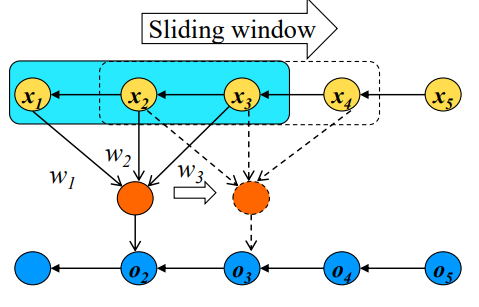
\includegraphics[scale=0.5]{26.png}
\end{center}
We will call this a "time-delay NN": weights are tuned as usual by learning and there's weight sharing.
\paragraph{2D convolution} Using a $n\times n$ kernel (\textbf{local receptive field}), we traverse the image with 1px shifts (\textbf{stride}), with padding used to treat the border.\begin{center}
	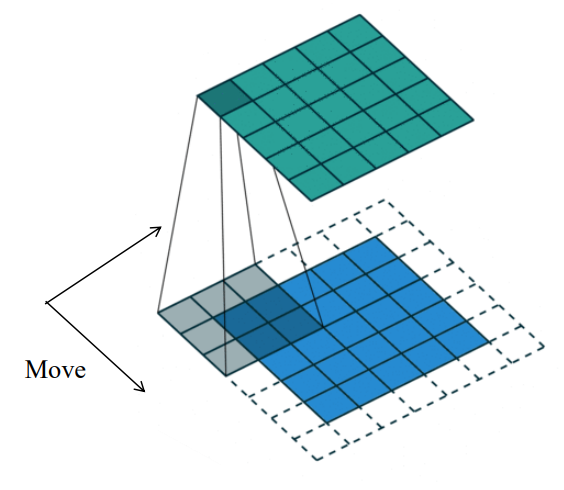
\includegraphics[scale=0.5]{27.png}\\
	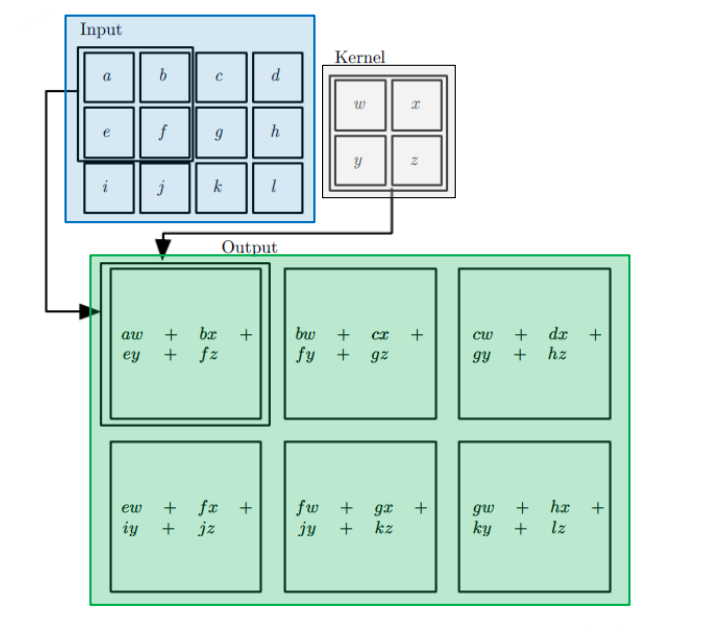
\includegraphics[scale=0.5]{28.png}
\end{center}
With a 2D image $I$ and a 2D kernel $K$ $$S(i,j) = (I*K)(i,j)=\sum_m\sum_n I(m,n)K(i-m,j-n)$$ or alternatively $$S(i,j) = (I*K)(i,j)=\sum_m\sum_n I(i+m,j+n)K(m,n)$$
The units weights are a \textbf{filter}, trained to detect some features in the image:
\begin{list}{}{}
	\item \textbf{Local and small receptive field} (kernel): with this architecture constraints, learned "filters" produce the strongest response to a spatially local input pattern
	\item The \textbf{same unit}/filter is \textbf{applied across the entire image}: this allows for features to be detected regardless of their position in the visual field, thus constituting the property of \textbf{translation invariance}
	\item \textbf{Learnable filters}: we can learn the filters that in traditional algorithms for image processing were hand-engineered. This independence from prior knowledge and human effort in feature design is a major advantage.
	\item \textbf{Stacking many layers}: feature maps unit represent larger and larger areas of the original image (assembling areas of the previous feature maps).
\end{list}
\paragraph{Pooling} So we reduce the feature map by subsampling (see before), or by operating a mean (average or weighted average), or by a max pool operation over the neighbors of each input. In practice, instead of producing a value for each input pixel, we produce a value for a rectangular set of pixels taking the mean or the max of the kernel/neuron outputs.
\begin{center}
	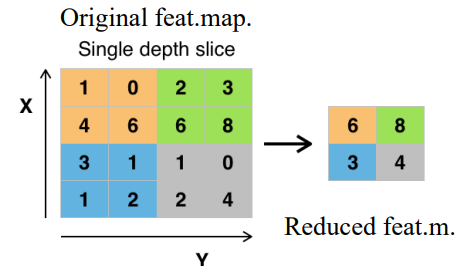
\includegraphics[scale=0.5]{29.png}\\
	Max pooling with a $2\times2$ filter and stride of $2$
\end{center}
Pooling also further helps to make the representation become approximately invariant to small translations of the input.
\paragraph{Overview} CNNs exploits weight sharing to setup a shifting windows or \textbf{local field} of the units over a segment of the input signal, also extended to 2D images and re-apply for many layers (\textbf{feature maps}).
\paragraph{Advantages}
\begin{list}{}{}
	\item \textbf{Local connections and weight sharing}: detect local patterns and invariant to translations, helping in reducing the number of free-parameters.
	\item \textbf{Pooling}: helps reducing the dimension of the representation (in each layer, so a pyramid of layers), also helps to small shifts and distortions
	\item Historical instance of deep neural network, progressively abstracting features from images.
\end{list}
\paragraph{How to use?} Training is typically made by backpropagation, with the many heuristics that we studied and some specializations for weight sharing, pooling ecc\ldots\\
Given the typical usage of huge networks and large amount of data, many hyperparameters are fixed by experience and expert suggestion, as it would be very expensive to run cross-validation over a large set of hyperparameters.
\paragraph{Modern CNNs} There are many variants and specialized architectures and models for image processing, and efficient implementations through tensor representation of matrices, exploiting GPUs. Even using the features of models already trained with large benchmarks: many pre-trained CNNs for image classification, segmentation, face recognition and text detection are available.
\paragraph{Parallelize linear operations on GPU} Matrix multiplication (i.e. dot product) is a typical linear operation performed efficiently on GPU. It can be parallelized by parallelizing the sum $(AB)_{ij} = \sum_{k=1}^m A_{ik}B_{kj}$ or a set of independent products $A_{ik}B_{kj}$ for each $i,j$\\
In computer programming, a \textbf{tensor} is a multi-dimensional matrix with a linear operation called \texttt{tensordot}. In many libraries such as \textbf{TensorFlow} we can use tensors and perform linear operations as \texttt{tensordot}s between them.
\subsection{Deep Learning}
\paragraph{Framework} "\textit{Deep learning  allows computational models that are composed of
multiple processing layers to learn representations of data with multiple levels of abstraction. These methods have dramatically improved the state-of-the-art in speech recognition, visual object recognition, object detection and many other domains}".\\
Starting from 2010, deep learning architectures are no longer unfeasible, thanks to the availability of large datasets, powerful computing systems\ldots\\
Deep learning is a \textbf{general framework} which includes different models:
\begin{list}{}{}
	\item Deep Neural Networks
	\item Convolutional Neural Networks
	\item Deep Belief Networks and Generative Approaches
	\item Recurrent/Recursive Neural Networks
	\item \ldots
\end{list}
This contrasts with "shallow models", e.g. neural networks with few layers.
\paragraph{Implement} Many approaches, basically by building MLPs with many layers and, for example, pre-training techiniques. Common aspects among approaches:
\begin{list}{}{}
	\item \textbf{Multiple layers} of nonlinear processing units
	\item Supervised or unsupervised \textbf{learning of feature representations in each layer}, with the layers forming a \textbf{hierarchy from low-level to high-level features}, giving different levels of abstraction
	\item Hence, hierarchical \textbf{sparse/distributed representation} of the input data
\end{list}
\subparagraph{Hierarchical Abstraction} Unsupervised or semi-supervised feature learning and hierarchical feature extraction \textbf{instead of features engineering}: moving towards the concept of "learning representations of data".\\
The abstract features can be "reused" at the higher levels: \textbf{combine to generalize} to unseen during training.
\paragraph{Techniques} In general, deeper networks are able to use less units in each layer, so less parameters and less training data to achieve a good generalization. But, many layers can be harder to train, hence emphasis on methods to improve
\begin{list}{}{}
	\item gradient descent (also due to gradients vanishing/exploding through layers)
	\item regularization (due to large networks)
	\item better exploitation of data
\end{list}
\paragraph{Do we \textit{need} many layers?} The general idea is that when a function can be compactly represented by a deep architecture, in might need a very large architecture to be represented by an insufficiently deep one.\\
An example from logic circuits: a two-layer circuit of logic gates can be represented by any boolean function, and any boolean function can be written as a sum of products (\textbf{disjuntive normal form}, $\wedge$ gates on the first layers with optional negation of inputs and $\vee$ gates on the second layer). With depth-two logical circuits, most boolean functions require an exponential (in input size) number of logic gates to be represented.\\
Examples: the parity function (return $1\Leftrightarrow$ there are an odd number of 1 over $N$ binary inputs) with 2 inputs can be done with 3 gates, with 3 inputs 5 gates, with $N$ inputs $2^{N-1}+1$ gates, exponential. If we use $\log N$ layers, we have fewer gates. However this doesn't hold for all classes of functions.\\
The \textbf{universal approximation theorem} is a fundamental contribution, it shows that 1 hidden layer is sufficient in general, but doesn't assure that a "small number" of units could be sufficient and it also doesn't provide a limit on such number. For many function families it's possible to find boundaries on such number and "\textbf{no flattening}" results (on efficiency): cases for which the implementation by a single hidden layer world require an exponential number of units (in terms of $n$ input dimension) or exponential non-zero weights, while more layers can help for the number of units/weights and also for learning.
\subparagraph{Examples} Cases with an exponential number of units are for example classes of problems requiring one hidden units corresponding to each input configuration that needs to be distinguished. For example, the number of possible binary functions on vector $v\in\{0,1\}^n$ is $2^{2^n}$ and selecting one such function requires $2^n$ bits which in general requires $O(2^n)$ degrees of freedom. It's a practical issue for the dimension of the network, but also implies that it's difficult to learn complex tasks with few examples.\\
On the other side there are families of functions that can be approximated efficiently by an architecture with depth greater than some value $d$, but which would require a much larger model if the depth is restricted to be $\leq d$. There's in general \textbf{no guarantee} that your task share this property.
\subparagraph{Theoretical Analysis} Deep models can exploit the \textbf{compositionality} of internal representation: an exponential gain in representation power, due to the fact that simpler concepts represented in a layer of the network can be exploited as primitives by the next layer to represent more complex concepts, avoiding explicit combinatorial representation and learning of features.\\
More in general, but it's an open theoretical research topic:
\begin{list}{}{}
	\item No-flattening results: no-flattening theorems, compositional functions that can be well implemented by a deep neural network cannot be implemented retaining the same efficiency while flattening the neural network
	\item A complete list of no-flattening theorems would show exactly when deep networks are more efficient than shallow networks
\end{list}
So, deep networks can be seen as compact models with respect to potentially larger shallow models for the task (even exponentially more compact). Hence more efficient, not just from the computational point of view but from the learning point of view too: less units and less weights help learning on complex tasks to achieve good generalization with less examples.
\subparagraph{Inductive Bias} Choosing a deep model encodes a very general belief that the function we want to learn should involve composition of several simpler functions. If our task matches this bias, then of course the deep shape of the learner is suitable, and it happens that generalization is better due to the use of many layers. Typical examples are: the structure of images (composition of sub-graphical parts), the structure of language (text and speech), music\ldots new fields are being discovered.\\
This doesn't apply to all data and tasks, of course. Also note that it's still a quite general bias, much more than other ad hoc constraints.
\subparagraph{Curse of Dimensionality} Many learners rely on local approximation (K-NN, local kernels, decision trees\ldots), but often the smoothness assumption (or local consistency) is not enough. They need training examples to generalize the surrounding and they may need many examples: $O(k)$ examples to distinguish $O(k)$ regions, or exponential number of regions (in $k$) with additional assumptions.\\
To approach this, one can make strong, task-specific assumptions, loosing the generality. Instead, the deep learning framework chooses a quite general inductive bias related to composition of functions: we assume that the data was generated by the composition of factors or features, potentially at multiple levels in hierarchy. This allows to:\begin{list}{}{}
	\item achieve a potentially exponential gain between number of examples and number of regions that can be distinguished
	\item generalize non-locally
	\item learn with less examples
\end{list}
\subparagraph{Practical issues} How many layers? How many units? Model selection!\\
In general, for deep learning: deeper network often with less units, so less parameters, so less training data. But many layers are harder to optimize during learning (exploding/vanishing gradients\ldots)
\paragraph{Representation Learning} "\textit{Representation learning is a set of methods that allows a machine to be fed with raw data and to automatically discover the representations needed for detection or classification}.".\\
Deep learning methods are representation-learning methods with multiple levels of representation. But this concept is more abstract an can be applied to many models, and neural networks in general.\\
This is in most cases referred to raw data such as images or texts.
\subparagraph{Basic ideas} Many information processing tasks can be very easy or very difficult, depending on the representation of the information (this applies to every field of computer science).\\
In Machine Learning, a good representation is one that makes a subsequent learning task easier. The \textbf{manual design of features} is difficult, even decades for specific communities (languages, images,\ldots). Supervised learning in a deep neural network is an example that leads to an \textbf{automatic representation} at every hidden layer, taking on properties that make the output layer task easier.
\subparagraph{Obtaining or exploiting hidden representation} The historical case in obtaining the hidden representation is the semi-supervised learning: we can learn a representation for the unlabeled data and then use it to solve supervised tasks (\textbf{pretraining approaches}).\\
To exploit the hidden representation, we can use the learned representation for other tasks (\textbf{transfer learning approaches})
\subsubsection{Implementing Deep Learning} Many approaches. Let's start with a simple one: building a multi-layer perceptron with many layers and pretraining techiniques.
\paragraph{Pretraining} The first approach to make the training of a deep supervised network possible was the \textbf{Greedy Layer-Wise Unsupervised Pretraining}: unsupervised learning as pretraining to capture the shape of the input distribution. It makes training the whole network easier, used by autoencoders.\\
Each layer is optimized independently (\textit{greedy layer-wise}) in an \textit{unsupervised} way, constituting a \textit{pretraining} for the final fine-tuning of the network. Works in terms of: good initialization strategy, regularization (in terms of discovering features that simplify the unsupervised process, which can be a more appropriate regularization technique when the underlying functions are "complicated" and shaped by regularities of the input distribution) and reducing the variance of the estimation.
\paragraph{Autoencoders} A neural network that is trained to attempt copy its input to its output. Internally, it has an hidden layer $h$ that describes a code used to represent the input. The network may be viewed as consisting of two parts: an encoder function $h = f(x)$ and a decoder that produces a reconstruction $r = g(h)$.\\
There many forms of autoencoders, for example:
\begin{list}{}{}
	\item \textbf{Undercomplete}: hidden layer smaller than the input.\\
	Forced to capture the most salient features of the training data by architectural constraints.
	\item \textbf{Overcomplete}: hidden layer bigger than the input.\\
	Regularization make the constraint for sparsity of the representation, robustness to noise and other properties of interest beside the trivial input-output copy capability.
\end{list}
Unsupervised!
\subparagraph{Layer-Wise Pretraining} Unsupervised, it can exploit also unlabeled data for the layer by layer training.
\begin{center}
	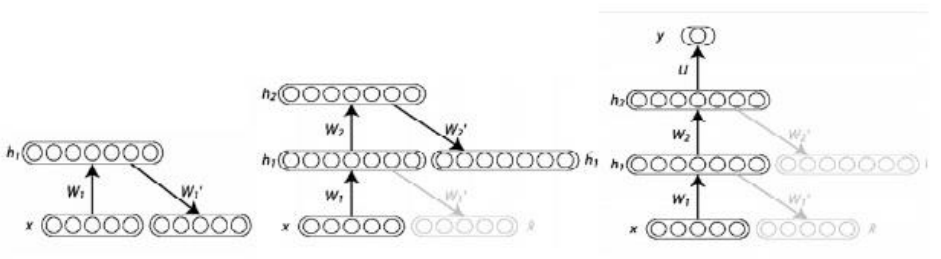
\includegraphics[scale=0.5]{30.png}
\end{center}
\begin{enumerate}
	\item Train the first layer as an autoassociator to minimize the reconstruction error of the raw input (unsupervised because we only need unlabeled examples)
	\item The hidden units outputs in the autoassociator are now used as input for another layer, also trained to be an autoassociator (again, unsupervised)
	\item Iterate 2. to add the desired number of layers
	\item Take the last hidden layer output as input to a supervised layer and initialized its parameters (either randomly or by supervised training, keep the rest of the network fixed)
	\item Fine-tune all the parameters of this deep architecture with respect to the supervised criterion
\end{enumerate}
The hope is that the pretraining has put the parameters of all the layers in a region from which a good local optimum can be reached by local descent. Despite many initially successful cases, the general role of pretraining is \textbf{nowadays under critical revision by researchers}.
\subparagraph{Needed?} Pretraining can yield improvements for some tasks, but not in other. It allowed to start deep learning, but its difficult to be managed.
\paragraph{Transfer Learning} Using the representation discovered in a model to improve another model. We assume there exist features that are useful for the different settings or tasks, corresponding to underlying factors that appear in more than one setting. But also we can use a trained model for another task, with same inputs but different targets (\textbf{multi-task learning}), or changing the input domain but sharing features (\textbf{domain adaption}), or take advantage of pre-training models from a larger dataset\ldots (note that the bold terms are subfields of machine learning)
\subparagraph{Example of pretrained networks}
\begin{list}{}{}
	\item \textbf{AlexNet}, a CNN that has been trained on $\simeq$ 1.2 million images, classifying them on 1000 categories: as a result, this model has learned rich feature representations for a wide range of images.\\
	It has 5 convolutional layers and 3 fully connected layers. Its learned features can be transfered to new classification tasks, e.g. by replacing the last 3 layers for your task and train those new layers.
	\item There are many pretrained CNNs for image classification, segmentation, face recognition and text detection.\\
	AlexNet in matlab, also MatConvNet, VGG, ResNet, GoofLeNet\ldots and similarly for other DL libraries such as Keras\ldots
\end{list}
\paragraph{Distributed Representation} "\textit{In a distributed representation, their elements (the features) are not mutually exclusive and their many configurations correspond to the variations seen in the observed data.}"\\
Deep learning methods exploit distributed representation with multiple levels of representation, but the concept is more abstract and can be applied to many models.\\
An example of \textbf{symbolic representation} is the \textbf{one-hot representation}: one element is 1, the others are 0 and the distance between two elements is always $\sqrt{2}$. With a \textbf{distributed representation} we have a dense vector of real numbers, and each symbol or concept is represented as the set of unit activations: this allows to share similarities and some learned features among concepts. The distance between two concepts reflects the meaning, and their similarity.
\begin{center}
	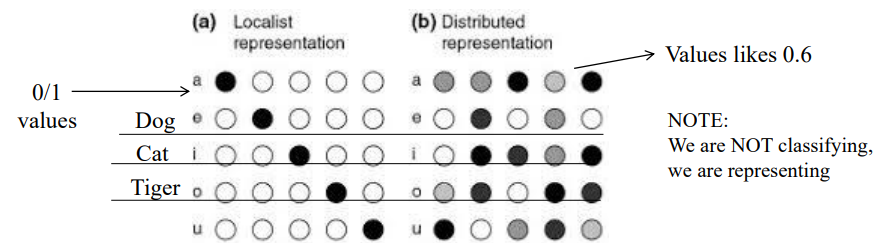
\includegraphics[scale=0.75]{51.png}
\end{center}
\subparagraph{Input or internal representation?} Symbolic and distributed refers to the input or the internal representation? We are talking in general, but \textbf{learning acts on the internal representation}. In general, distributed representation is used:
\begin{list}{}{}
	\item In input if you have a background knowledge to build it (if it's done improperly then it could hamper the task solving)
	\item Automatically, by learning, if distributed representation can be used internally in the model (e.g. hidden neural network layers)\\
	Typically, one-hot is used for the input and the model is free to develop internally the distributed representation needed for the task at hand
\end{list}
\subparagraph{Count the difference} Distributed representation can represent $n$ features with $k$ values to describe $k^n$ different concepts.
\subparagraph{Sharing attributes} By sharing a learned feature we can share its concept, disentangling it from the task.
\subparagraph{Example} 4 concepts: blue car, blue bike, red car, red bike. There's no need for 4 neurons, just 2 are enough: a neuron for blue/red and a neuron for car/bike. The neuron describing redness is able to learn about the concept of redness from images of cars and bikes, not just one.\\
If we share that neuron, we share the concept of redness.
\subparagraph{Beyond Neural Networks} The debate on distributed representation extend to the debate between \textbf{logic-inspired paradigms} and \textbf{neural network-inspired paradigms} for cognition.
\subparagraph{Interpretability} Less easy for distributed representation.
\paragraph{Deep Distributed Representation} Deep learning exploits distributed representation through many layers, obtained by composing different levels of abstraction or by a hierarchy of reused features. This compositionality, as already discussed, can lead to further exponential boost in efficiency. Globally, deep learning learn a distributed representation of the data by disentangling shared causal factors that generates the data through different levels of abstraction.
\pagebreak
\paragraph{Deep Learning Techniques} Key techniques for training a layered neural network:
\begin{list}{}{}
	\item Originally: pretraining approaches
	\item Nowadays:
	\begin{list}{}{}
		\item \textbf{SGD} with momentum, with decay on $\eta$ or minibatch, or Adam\ldots
		\item \textbf{ReLU} activation functions on hidden units
		\item \textbf{Cross-Entropy} (max $\log$-likelihood) loss with softmax for output layers, also to avoid saturation and small gradient effects
		\item \textbf{Regularization}: early stopping and weight decay, also drop-out and batch normalization (for CNN and sigmoids)
	\end{list}
\end{list} 
\paragraph{Gradient Issues} The magnitude of the gradients, as its backpropagated through the many layers, suffers from two main issues:
\begin{list}{}{}
	\item If the weights are small, the gradient shrinks exponentially (\textbf{vanishing gradient})
	\item If the weights are big, the gradient grows exponentially (\textbf{exploding gradient})
\end{list}
Some approaches include the \textbf{gradient clipping}: if $||g||> v$ then $g = \frac{vg}{||g||}$ with $g$ being the gradient and $v$ the norm threshold, as to move in the gradient direction but bounding the weight update.\\
Most of the heuristics try to deal with the problem of vanishing gradient that hampers the training in early deep neural network in the low layers. Traditional activation functions, such as the hyperbolic tangent, have gradients in the range of $(-1,1)$ and the backpropagation computes gradients by the chain rule repeated through the layers. This has the effect of multiplying $n$ of these small numbers to compute gradients of the "front" layers (closer to the inputs), in a $n$-layer network: the gradient decreases exponentially with $n$, with the result of a very slow training in the front layers. Same with big weights (exploding gradients), but less frequent.\\
To deal with this, many approaches: Rprop, short-cut connections, randomized neural networks\ldots let's see the new ones.
\subparagraph{ReLU} \textbf{Rectified Linear Unit}: $f(x) = \max(0,x) = \left\{\begin{array}{l l}
0&\text{if }x< 0\\
x&\text{if }x\geq 0\\
\end{array}\right.$
\begin{list}{}{}
	\item \textbf{Sparse activation}: in a randomly initialized network, only about 50\% of hidden units are activated (non-zero output)
	\item \textbf{Efficient gradient propagation} with respect to vanishing and exploding effects
	\item \textbf{Efficient computation}: only comparison, addition and multiplication
	\item \textbf{Faster and effective training of deep neural architectures}
	\item But it's non differentiable in 0!
\end{list}
Used in deep learning since 2009 due to the simplified and better gradient propagation through many layers and the avoiding of saturation effects of sigmoidal functions. Non differentiable in 0, but often assumed to be 0 for the left derivative and 1 for the right derivative: the approximation is acceptable and safe because there's already an approximation for $x$ input, so unlikely to be $x=0$ effectively.\\
Beyond ReLU there are:
\begin{list}{}{}
	\item ELU (Exponential Linear Unit), $f(\alpha,x)=\left\{\begin{array}{l l}
	\alpha(e^x - 1)&\text{if }x \leq 0\\
	x&\text{if} x > 0
	\end{array}\right.$
	\item Leaky ReLU $f(x) = \left\{\begin{array}{l l}
	0.01x&\text{if }x < 0\\
	x&\text{if }x \geq 0 
	\end{array}\right.$
\end{list}
\paragraph{Batch Normalization} Method that normalizes each batch by calculating each individual batch statistic such as mean and variance for each layer (\textbf{reparametrization}): normalize each matrix (databatch $\times$ activation of units) with mean and variance, by shifting values to zero-mean and unit variance, and include it in backpropagation.\\
Normalizing inputs is a standard approach, batch normalization helps by making the data flowing between intermediate layers to stay normalized. It has a regularization effect, achieving faster learning and higher accuracy for deep learning.
\paragraph{Dropout} Method that randomly selects and "ignores" a subset of the network units during its training. Can be explained in terms of:
\begin{list}{}{}
	\item Ensembling: implicit bagging, different sub-networks
	\item Regularization
\end{list}
Bagging is the combination of many classifiers/models: train $n$ classifiers/models on different subsets of the TR and differentiate each training using bootstrap (resampling with replacement). Dropout aims to approximate this process, with an exponentially large number of sub neural networks (while still having a single network at test time), while also aiming at maximizing the diversity of the ensemble preventing complex co-adaptions on training data.\\
A basic algorithm:
\begin{list}{}{}
	\item Each time an example is loaded into a minibatch, we randomly sample a different binary mask to apply to all of the input and hidden units in the network.\\
	The mask is sampled independently for each unit, and the probability of a mask value of 1 (causing the unit to be included) is an hyperparameter, typically 0.8 for input units and 0.5 for hidden units.
	\item The forward propagation, back propagation and the learning algorithm are done as usual (only on a subset of units at the time)
	\item The removed nodes are then reinserted into the network with their original weights.
\end{list}
There's parameter sharing among sub networks: in each single step only a small fraction of the possible sub networks are trained, but the parameter sharing causes the remaining sub networks to arrive at good settings of parameters.\\
It also has regularization effect:\begin{list}{}{}
	\item Avoids training all units on all training data, reducing units interactions
	\item Variance reduction as for bagging
	\item Insert structured noise\\
	For example, recognize a face with the hidden unit for the nose, compare it with standard regularization by adding deformed inputs with random noise.
\end{list}
Moreover, it regularizes each unit to be not merely a good feature but a feature that is good in many contexts (different sub-networks). It can be shown to be equivalent to L2 weight decays using a different $\lambda$ for each input, can be used for any model that uses distributed representation and SGD training and can be extended to any kind of random modification.
\paragraph{L1 Regularization}
Using the L1 norm (sum of absolute values) instead of the L2 norm in the penalty term. Favorite features elimination (weight zero) with respect to L2, which often only shrinks the weights without setting any of them to zero. This produces simpler final models.
\paragraph{Adversarial Training} \textbf{Generative Adversarial Network}: two neural networks contesting with each other, one network generates candidates and the other evaluates them.
\subsection{Random Weights Neural Networks} A randomized approach employs a degree of randomness as part of its constructive strategy. Randomness can be seen as an effective part of ML approaches: can enhance several aspects of Machine Learning methodologies (data processing, learning, hyperparameter selection\ldots) and randomization can be a key factor in building efficient Machine Learning models.\\
Randomness can be present at different levels: to enhance predictive performance and/or to alleviate difficulties of classical Machine Learning methodologies. For example: data splitting to avoid overfitting (hold-out, K-fold,\ldots), data generation, learning (observation order for example with shuffling minibatches) and hyper-parameters selection (for example with random selection).
\paragraph{Overview} Is it possible to exploit MLP/RNN architectures without long training cycles in the hidden layers? Long tradition of randomized neural networks, random weights, random projections\ldots (e.g. Random Vector Functional Link Neural Network, RVFL). Recently, popularization of other schemes including ELM (Extreme Learning Machine).\\
Basic idea: a network containing \textbf{randomly connected hidden layers}, i.e. \textbf{weights are fixed after random initialization} and \textbf{only the output weights are trained}.
\paragraph{Structure}\begin{list}{}{}
	\item \textbf{Input}
	\item \textbf{Untrained hidden layer}\\
	Non-linearly embeds the input into a high-dimensional feature space, where the problem is more likely to be solved linearly. Theoretically grounded on the Cover's Theorem
	\item \textbf{Feature representation $\phi$}
	\item \textbf{Trained readout layer}\\
	Combines the features in the hidden space for output computation. Typically implemented by linear models
	\item \textbf{Output}
\end{list}
\paragraph{Cover's Theorem} A complex pattern-classification problem, cast in a high-dimensional space non-linearly, is more likely to be linearly separable than in a low-dimensional space, provided that the space is not densely populated.\\
In particular, using a deterministic mapping: assuming $l$ examples, lift them onto the vertexes of the $l-1$ dimension triangle (simplex), so that now every binary partition of the samples is linearly separable.\\
It's the \textbf{same property exploited by kernels}.
\subsubsection{Feedforward Ranbdomized Neural Networks} Input-output relation is implemented through an untrained hidden layer, which implements a randomized basis expansion.
\paragraph{Pros and cons} Large set of hidden unit plays an interesting role: projection non-linearly expands the dimension of an input vector as to make the data more separable. A large number of units can provide sufficient "basis expansion" to solve the task. Also it's extremely efficient, and many variants and improvements exists (incremental learning adding hidden neurons, pruning\ldots\\
Of course smaller models, with smaller numbers of adaptive units (basis functions) trained on the specific task at hand appear more elegant (\textbf{random features} vs \textbf{learned features} approaches)
\paragraph{Suitable for}\begin{list}{}{}
	\item \textbf{Big data} due to extreme efficiency
	\item \textbf{Tiny implementations} for distributed embedding systems in resource limited devices
	\item \textbf{Deep Learning}\\
	Randomized neural networks can alleviate the computational burden of training. Randomized CNN approaches and also Deep Feedforward Randomized NN: networks consisting in stacks of RVFL/ELM modules.
	\item \textbf{Recurrent Randomized Neural Networks}, where efficiency of training is more demanding respect to MLP
\end{list}
\subsection{Unsupervised Learning in Neural Networks}
\paragraph{Unsupervised Learning} No teacher! TR = set of unlabeled data $\langle x\rangle$
\subparagraph{Tasks}\begin{list}{}{}
	\item \textbf{Clustering}, find natural groupings in a set of data
	\item \textbf{Dimensionality Reduction}/Visualization/\textbf{Preprocessing}: multidimensional data are projected in a lower dimensional space (principal component analysis, multi-dimensional scaling\ldots)
	\item \textbf{Modeling the data density}
\end{list}
\paragraph{Clustering} We focus on clustering, which is a problem that has been addressed in many contexts and by researchers in many disciplines. Thousands of different algorithms, but we go directly to a simple approach and a historical NN model: the \textbf{SOM/Kohonen maps}. We use a vector quantization perspective for partitioning clustering.
\begin{center}
	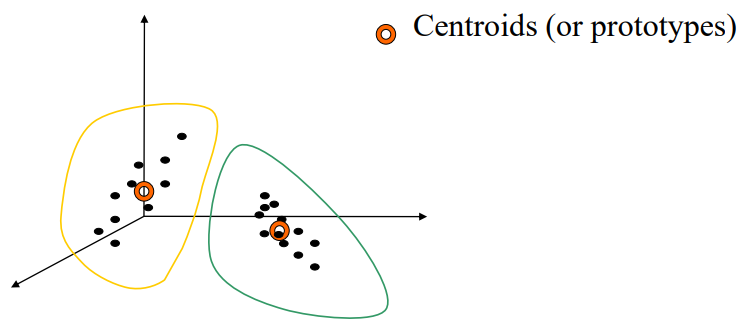
\includegraphics[scale=0.5]{31.png}
\end{center}
\subparagraph{Similarity Measures} The metric is very important, the assumed distance tells us which are the similar examples (\textbf{pattern proximity}), and the clustering algorithm decide the grouping using that metric.\\
Many possible metric, Euclidean metrics are popular but it's just a choice.
\paragraph{Vector Quantization} Vector quantization techniques encode a data manifold, e.g. a submanifold $V\subseteq \mathbb{R}^n$, using only a finite set $w=(w_1,\ldots,w_k)$ of \textbf{reference/codebook vectors} $w_i\in \mathbb{R}^n$ with $i=1,\ldots,k$\\
A data vector $x\in V$ is described by the best matching or "winning" reference vector $w_{i^*(x)}$ of $w$ for which the \textbf{distortion error} $d(x, w_{i^*(x)})$ is minimal.\\
This procedure divides the manifold $V$ into a number of subregions $$V_i=\{x\in V\:|\:||x-w_i||\leq ||x-w_j||\forall\:j\}$$ called \textbf{Voronoi Polyhedra}, out of which each data vector $x$ is described by the corresponding reference vector $w_{i^*(x)}$
\begin{center}
	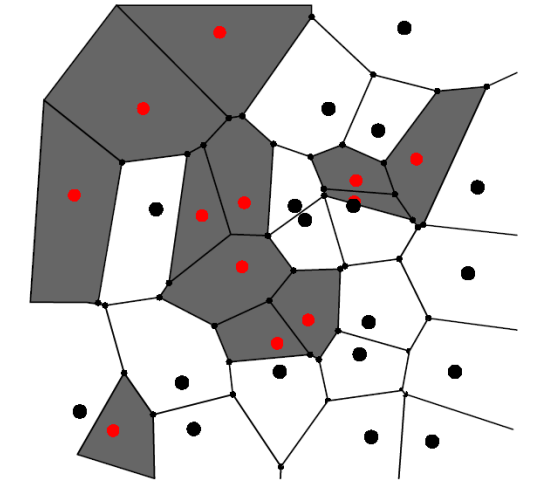
\includegraphics[scale=0.5]{32.png}
\end{center}
In general it's hard to compute: optimal vector quantization codebook is NP-complete.\\
Each cell consists of all points closer to the bold black/red points than to any other patterns. The segments of the \textbf{Voronoi Diagram} are all the points in the plane equidistant to two patterns.\\
For us, the problem is to find centers that minimizes the loss $E$ given the dataset.\\\\
Clustering has a more general objective of finding interesting/useful groupings of data. Interesting is often implicitly defined via the computational procedure by itself and not necessarily measured by the minimum quantization error. However, vector quantization provides an usefult framework and its algorithms can be used for clustering. We're going to use this perspective.
\subparagraph{Goal} Optimal partitioning of unknown distribution in $x$-space into clusters approximated by a cluster center or \textbf{prototype}.\\
I.e. a set of vector quantizers $x\rightarrow c(x) = w_{i^*(x)}$, from continous space to discrete space.\\
We evaluate the squared error distortion $d(x_i,c(x_i)) = ||x_i-c(x_i)||^2$
\subparagraph{Loss function} The average value over the distribution of inputs is the average distortion/reconstruction/quantization error: our loss function. $$E = \int f(d(x,w_{i^*(x)}))\cdot p(x)\:dx= \int||x-w_{i^*(x)}||^2\cdot p(x)\:dx$$
Discrete version: $$E = \sum_i^l\sum_j^K||x_i-w_j||^2\delta_{winner}(i,j)$$ with $\delta_{winner}(i,j)$ the characteristic function of the receptive field of $w_j = \left\{\begin{array}{l l}
1&\text{if }j\text{ is the winner for }x_i\\
0&\text{otherwise}
\end{array}\right.$ and $p(x)$ the probability distribution of $x$.\\
Minimizing $E$ is the vector quantization: minimize $E$ through an optimal choice of $w$, the set of reference vectors $w$ that minimizes $E$ is the solution of the vector quantization problem.\\
Note that the integrand of $E$ is not continuously differentiable: $w_{i^*(x)}$ have discrete changes, but derivatives can be computed locally by fixing $x$ in a Voronoi cell.
\paragraph{Online $K$-means} Taking the derivatives of $E$ in the discrete version with respect to the $w_j$ yields the learning rule of vector quantization.\\
The online version of $K$-means for any $x_i$ is $$\delta w_{i^*} = \eta\delta_{winner}(i,i^*)(x_i-w_{i^*})$$
with $\eta$ being the learning rate. The basic algorithm is:
\begin{enumerate}
	\item Choose $k$ cluster centers to coincide with $k$ randomly selected patterns or $k$ randomly defined points inside the hypervolume containing the set
	\item Assign each pattern to the closest cluster center (the winner)
	\item Recompute the cluster centers (geometric centroids, i.e. means) using the current cluster membership.
	\item If a convergence criterion is not met, go to step 2. Examples of stopping criteria are: no or minimal reassignment of patterns to new cluster centers, or a minimal decrease in squared error.
\end{enumerate}
Given the cluster centers $w_1,\ldots,w_k$ of dimension $n$ same as $x$, for each $x$ the winner is the nearest prototype $i^*(x) = arg\:min_i||x-w_i||^2$, so now $x$ belong to the cluster $i^*$.\\
For each cluster $i$ the new centroid is $w_i=\frac{1}{|\text{cluster}_i|}\sum_{j\:|\:x_j\in\text{cluster}_j}x_j$\\\\
This is the simplest and most common algorithm employing a squared error criterion, it's easy to implement and efficient in general.\\
The number $K$ of clusters to find must be provided and local minima of $E$ makes the method dependent on the initialization. Also it works well only with hyperspherical and compact clusters, and has no visualization properties (doesn't allow to project in a lower dimension space).
\paragraph{Softmax} To avoid confinement to local minima, a common approach is to introduce softmax adaptation rule: not only the winning reference is modified, but the adaption of $x$ affects all cluster centers depending on their proximity to $x$, typically with a step size that decreases with the distance $d(x,w_i)$. An instance of this strategy in neural networks is the Kohonen self-organizing maps, where the proximity among reference vectors is defined on a ordered map.
\subsubsection{Self-Organizing Maps} SOM neural networks are also called Kohonen maps. Consists of $N$ neurons located on a regular low-dimensional, usually 2D, grid. Each unit can be identified by the coordinates on the map, receives the same input $x$ and has a weight $w$.\\\\
SOM learns a map from an input space to a lattice of neural units. It's a topology preserving map: neighboring units respond to similar input pattern, datapoints close in the input space are mapped onto the same or nearby map units.
\paragraph{Usage} \begin{list}{}{}
	\item \textbf{Clustering}: clusters can be identified on the map.
	\item \textbf{Pattern recognition} and \textbf{vector quantization}: the input is transformed into the closest neuron weights, the reference vector.
	\item \textbf{Data Compression}: the input is transformed into the indexes, or digital codes, of the winner unit.
	\item \textbf{Projects and exploitation}: the distribution of the multidimensional data is visualized in a lower dimensional space (the 2D map)
\end{list}
\paragraph{Competitive learning} An adaptive process in which neurons gradually becomes sensitive/specialized to different input categories/set of examples.\\
Competitions among neurons for an input data, where the winner is allowed to learn more.
\paragraph{Learning algorithm}\begin{enumerate}
	\item The map is randomly initialized (weights)
	\item A sample input $x$ is drawn
	\item \textbf{Competitive Stage}: the winner is the unit (with $w$) most similar to $x$\\
The current input vector $x$ is compared with all the unit weights using an euclidean distance criteria. The standard SOM adopts a "winner takes all" strategy, with the winner being $i^*(x) = arg\:min_i||x-w_i||$ where $i$ is an index on the map (e.g. coordinate in 2D)
	\item \textbf{Cooperative Stage}: upgrade the weights of the units that have topological relationships with the winner unit (\textbf{softmax})\\
	The weight of the winning unit and the weight of the units in its neighborhood are moved closer to the input vector (Hebbian learning)\\
	At iteration $t$ $$w_i(t+1) = w_i(t) +\eta(t)h_{i,i^*(x)}(t)(x - w_i(t))$$ where $h(t)$ is the neighborhood function i.e. $h_{i,j}(t)$ is a function that decreases monotonically for increasing $||i-j||$ $$h_{i,i^*}(t)=\exp\left(-\frac{||r_i - r_{i^*}||^2}{2\sigma^2_{nh}(t)}\right)$$
	The neighborhood radius $\sigma$ and the learning rate are decreased as function of iteration $t$: wide at the beginning and then width and height slowly decreases during learning.
	\item Continues until convergence, when there are no changes
\end{enumerate}
\paragraph{Topological Order} The update rule of the cooperative stage is fundamental to the formation of topographically ordered maps. In fact, the weights are not modified independently of each other, but as topologically related subsets. For each subset similar kinds of weight updates are performed. For each step a subset is selected on the basis of the neighborhood of the current winner unit.\\
Hence topological information is supplied to the map because both the winning units and its lattice neighbors receive similar weight updates that allow them, after learning, to respond to similar inputs.\\
Formal proofs of ordering is difficult.
\paragraph{Visualization} The map can be used to visualize different features of the SOM and of the data represented. For example:
\begin{list}{}{}
	\item Density of the reference vectors
	\item Distance between prototype vectors of neighboring units
	\item Sammon maps\ldots
\end{list}
providing the SOM with easy interpretability.
\subsection{Recurrent Neural Networks}
\paragraph{"The Neural Network That Remembers"} With short-term memory, recurrent neural networks are able to remember, thus gaining amazing abilities. A recurrent neural network includes connections between neurons in the same hidden layer, some of which feed back on themselves.
\begin{center}
	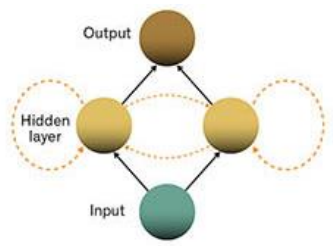
\includegraphics[scale=0.75]{33.png}
\end{center}
In \textbf{feedforward} neural networks, the direction of the data flow is input $\rightarrow$ output. In \textbf{recurrent} neural networks, we add \textbf{feedback loops} connections in the network topology. The presence of self-loop connections provides the network with dynamical properties, leaving a memory (states) of the past computations in the model: this allows us to extend the representation capability of the model to the processing of sequences (and structured data).\\\\
Whenever the output of the model depends on the history of the inputs, or the domain is composed by varying-size sequences, we talk about \textbf{sequential data}:
\begin{list}{}{}
	\item Dynamical processes
	\item Language
	\item Vision
	\item Temporal series
	\item Genomics
	\item \ldots
\end{list}
Recurrent neural networks nowadays are the reference approach for sequence processing, especially for state-of-the-art result in speech recognition/processing and text processing, or even music composition, text/speech generation\ldots\\
Sequences are examples of \textbf{structured data}: up until now we used vectors, which are examples of \textbf{flat data}, while sequences, trees, graphs are all structured data. So we have a new input domain and trasductions:
\begin{list}{}{}
	\item \textbf{Data}: discrete sequence of vectors (serial order, e.g. time)
	\item \textbf{Tasks}: sequence recognition/classification (single output at the end), sequence trasduction or next step prediction (each output is a vector)
\end{list}
\textbf{Trasduction} in the sequential domain is the mapping input sequence $\mapsto$ output value/sequence.
\subsubsection{Memory in neural networks}
\paragraph{Input Delay Neural Networks} Aim: output depends on the previous inputs, example of temporal processing in neural networks. We have finite memory, spatial approach. IDNN in time-delay are TDNN: delays are in the neural network connections to act as input memory. Finite-size shift register (\textbf{sliding window})
\begin{center}
	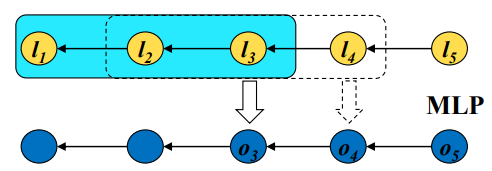
\includegraphics[scale=0.5]{34.png}
\end{center}
CNN extends this idea to 2D images. We must know the window dimension in advance, and the number of weights depends on the buffer size.
\paragraph{Recurrent Unit} Uses the current unit plus \textbf{states information}. Recurrent neural unit with feedbacks in the architecture.
\begin{center}
	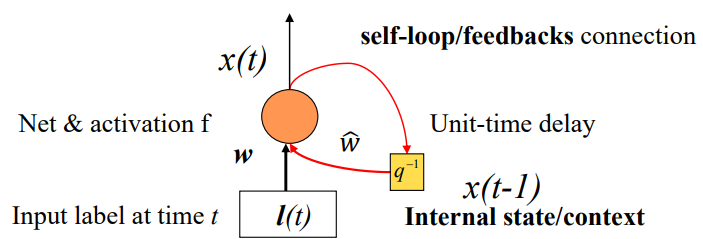
\includegraphics[scale=0.5]{35.png}
\end{center}
$$x(0) = 0$$
$$x(t) = \tau(l(t),x(t-1)) = f(wl(t) + \overline{w}x(t-1) + \Theta)$$
With $f$ sigmoidal activation function, $\overline{w}$ recurrent weight and $\Theta$ bias. The state summarize the past information, the \textbf{context}: the encoding of the past is adaptive (free weights of the model).
\paragraph{State Transition System - Recurrent Model} Given $x(0) = 0$, $\left\{\begin{array}{l}
x(t) = \tau(x(t-1),l(t))\\
y(t) = g(x(t), l(t))
\end{array}\right.$
\begin{center}
	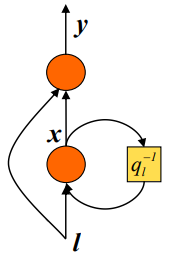
\includegraphics[scale=0.5]{36.png}
\end{center}
$\tau$ is the \textbf{state transition} function realized by a neural network. The states summarizes the past inputs. $x$ can be a set of states.
\paragraph{Recurrent Neural Networks} \begin{center}
	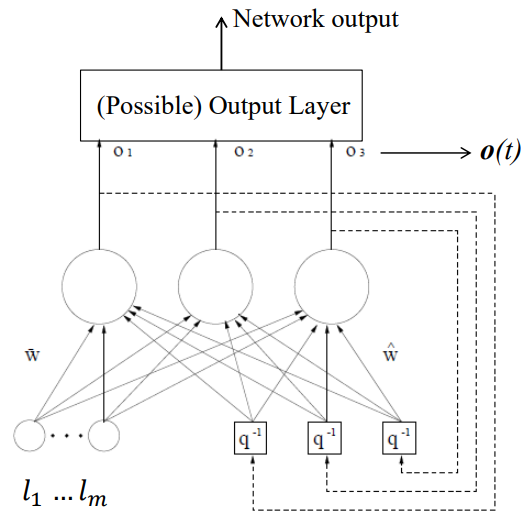
\includegraphics[scale=0.5]{37.png}
\end{center}
\textbf{Properties}: many architectures are possible, however the simple RNN seen before is already powerful, they are \textbf{universal approximators} of non-linear dynamical systems and are \textbf{Turing-equivalent} (e.g. any automata can be simulated).\\
RNN are based on the following assumptions:
\begin{list}{}{}
	\item \textbf{Causality}: a system is causal if the output at time $t_0$ (or node $v$) only depends on inputs at time $t<t_0$ (or depends only on $v$ and its descendants).\\
	Necessary and sufficient for internal state.
	\item \textbf{Stationarity}: time invariant (after model training), i.e. the state transition function $\tau$ is independent of node $v$ of the sequence.\\
	This means that $\tau$ is the same in any time $t$, regardless of the dimension of sequences.
	\item \textbf{Adaptivity}: transition functions are realized by neural networks with free weights, hence they are \textbf{learned} from data.
\end{list}
\paragraph{Unfolding} Is the \textbf{unrolling through time the same model}.
\begin{center}
	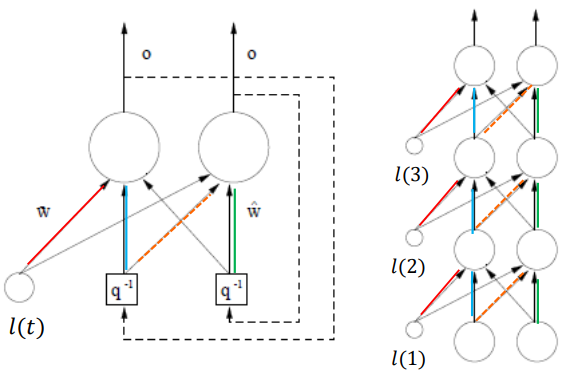
\includegraphics[scale=0.5]{38.png}
\end{center}
We can build a feedforward MLB (called \textbf{encoding network}) equivalent to the RNN given a specific input sequence. It's the replica of the model for each step, and stationarity $\Rightarrow$ weight sharing across unfolded layers. On this encoding network we can apply the backpropagation algorithm.
\paragraph{Learning Algorithms} The learning algorithm must take into account the set of encode transitions developed by the model for each step of the inputs. \textbf{BPTT} (Backpropagation Through Time) and \textbf{RTRL} (Real Time Current Learning) are \textbf{supervised} learning algorithms designed for recurrent neural networks. In different style, they compute the same gradient values of the output errors across an \textbf{unfolded} network that is equivalent to the recurrent one (encoding network). The vanish of gradients over this deep network can make difficult to learn long-term dependencies.
\paragraph{Advanced Models} It's a rapid growing research field, with many variants:
\begin{list}{}{}
	\item \textbf{LSTM} (Long Short-Term Memory): tries to solve the vanishing gradients problem by using "gate units" able to select the past/gradient flow. Not suitable for short series, these are born to address the need to retain long term memory.
	\item \textbf{GRU} (Gated Recurrent Units): simplified LSTMs
	\item \textbf{BRNN} (Bi-Directional RNN): to consider both the left and right context
	\item But also, to deal with gradient vanish issues: Hessian-free optimizers, pre-training techniques\ldots
\end{list}
\paragraph{Related Approaches} \begin{list}{}{}
	\item SOM/Unsupervised NN for sequential domains
	\item \textbf{HMM} (Hidden Markov Models): models the probability distribution of state transition
	\item \textbf{Randomized NN}: \textbf{reservoir computing} and ESN
	\item Distance based models (string matching)
	\item Grammatical inference
	\item \textbf{ILP}
\end{list}
\paragraph{Towards ESN} We can exploit directly this state machine to encode sequences and then use it to learn the output mapping, even with random connected networks with fixed (untrained) random weights.\\
Fractal machine plus reservoir computing: very efficient with the capability to solve task well, under specific conditions. Ability to intrinsically discriminate among different input sequences in a suffix-based fashion, without adaptation of the recurrent parameters.
\subsection{Echo State Networks}
\begin{center}
	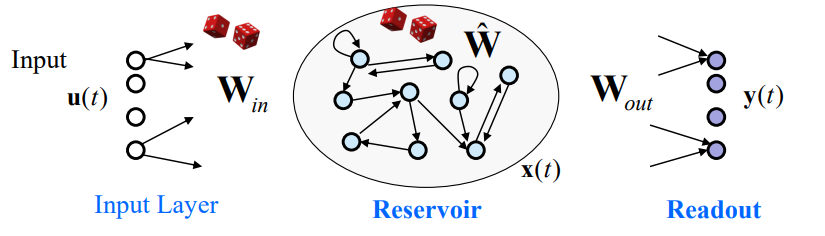
\includegraphics[scale=0.5]{39.png}
\end{center}
Paradigm to efficiently model recurrent neural networks. An Echo State Network consists of:
\begin{list}{}{}
	\item Large \textbf{reservoir} of sparsely connected recurrent units, \textbf{untrained} after a random initialization
	\item A simple feed-forward \textbf{readout} of linear units \textbf{trained} by efficient linear methods (e.g. ridge regression)
\end{list}
\textbf{Echo State Property}: contractivity of the state transition functions, limiting the spectral radius of reservoir weights (i.e. the stability of the dynamical system).
\paragraph{Recurrent plus deep} We can, combining the power of deep RNNs and the efficiency of ESN. Deep ESNs are under study, and deep layered organization of recurrent models show advantages in terms of: occurrence of multiple time-scale and increasing of richness of the dynamics (hierarchical).
\paragraph{Toward Structured Domains} Can we extend this recurrent approach to rooted trees? Yes.
\section{Structured Domains}
\paragraph{Why structured data?} Because data have relationships.\\
Vectors are examples of \textbf{flat data}, while sequences, trees, graphs are all examples of \textbf{structured data}. There are lots of examples:
\begin{list}{}{}
	\item Pattern recognition
	\item Language parsing (trees)
	\item Terms in first order logic (trees)
	\item Social networks
	\item Biological networks: proteins as nodes and the links represent interactions, or similarity
	\item Maps, graphs: networks of roads. Each node is a route segment, and edges are between segments that are consecutive on the same road or connected through an intersections. Example tasks: traffic predictions or estimated times or arrival
\end{list}
In the following we use this notation for graphs:
\begin{list}{}{}
	\item Nodes/Vertexes $v$, vectors, with labels. For example the node $v$ has label $d$, and $l(v) = l_d = [1,0,1,0,7]$
	\item Arc/Edges/Links can be oriented/directed or not
\end{list}
\paragraph{Graph Representations} There has been no systematic way to extract features or metrics relation between examples for structured domains. \textbf{Feature based} representations are incomplete (or strongly task-dependent), while \textbf{adjacent/incident matrix} representations or any other fixed-size representation have other issues (over-dimensionality, alignment among different graphs, topological orders which makes generalization difficult).\\
The ability to treat the proper inherent nature of the input data is the key feature for a successful application of the machine learning methodologies.\\
The goal is to \textbf{learn} a mapping between a structured information domain (SD) and a discrete/continuous space (\textbf{transduction} $T$): given a set of examples (graph, target), we can learn a \textbf{hypotheses mapping} $T$(graph). So instead of moving data to models (e.g. graphs into vectors, trees into sequences\ldots with alignment problems, loss of information, etc.) we \textbf{mode models to data}.
\paragraph{Classes}
\begin{center}
	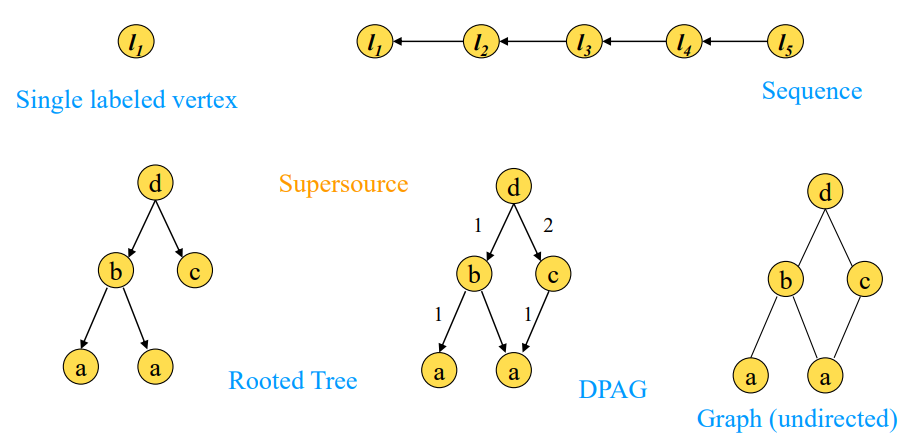
\includegraphics[scale=0.5]{40.png}
\end{center}\begin{list}{}{}
	\item \textbf{K-ary tree}: root and bounded out-degree ($k$) for each node (the number of children)
	\item \textbf{DPAG}: laveled direct positional acyclic graphs with supersource, bounded in-degree and out-degree ($k$)
\end{list}
\paragraph{Overview of SD learning}
\begin{center}
\begin{tabular}{c | c | c | c}
& \textbf{Symbolic model} & \textbf{Connectionist model} & \textbf{Probabilistic model}\\
\hline
\makecell{\textbf{Static}\\Attribute/value,\\real vectors} & \makecell{Rule induction,\\decision trees} & NN, SVM & \makecell{Mixture models,\\naive Bayes}\\
\hline
\makecell{\textbf{Sequential}\\Serially ordered\\entities} & \makecell{Learning finite\\state automata} & RNN & \makecell{Hidden Markov\\models}\\
\hline
\makecell{\textbf{Structural}\\Relations among\\domain variables} & \makecell{Inductive logic\\programming} & \makecell{RNN\\(kernel for SD)} & \makecell{Recursive Markov\\models}
\end{tabular}
\end{center}
\paragraph{Transductions}
From an input graph $g$, $T_{enc}$ produces $x(g)$ (possible internal representation/encoding) and with that produces the outpu $y(g)$ which type depends on the kind of transduction: a general transduction can be either
\begin{list}{}{}
	\item \textbf{Structure-to-Structure}, input and output $y(g)$ isomorphic
	\item \textbf{Structure-to-Scalar}, regression/classification
	\item Or in general can also be \textbf{non-isomorphic}
\end{list}
\subsection{Recurrent/Recursive Approaches for Trees}
\paragraph{RRNs} A state-transitions system with free parameters. Given $x(0) = 0$, the internal state is $\left\{\begin{array}{l}
x(t)=\tau(x(t-1),l(t))\\
y(t)=g(x(t),l(t))
\end{array}\right.$ and the states summarize the past information, with $\tau$ being the state transition function realized by a neural network with weights and sigmoidal functions.\\
Over time the state information increases:
\begin{center}
	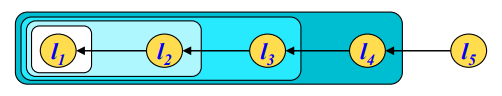
\includegraphics[scale=0.75]{41.png}
\end{center}
We can use RNNs to implement a bottom-up encoding of input trees, extending states for children of vertexes of the tree: \textbf{universal approximation} over the tree domain/DPAG
\begin{center}
	$$\left\{\begin{array}{l}
x(v)=\tau(x(\text{ch}[v]),l(v))\\
y(v)=g(x(v),l(v))
\end{array}\right.$$
	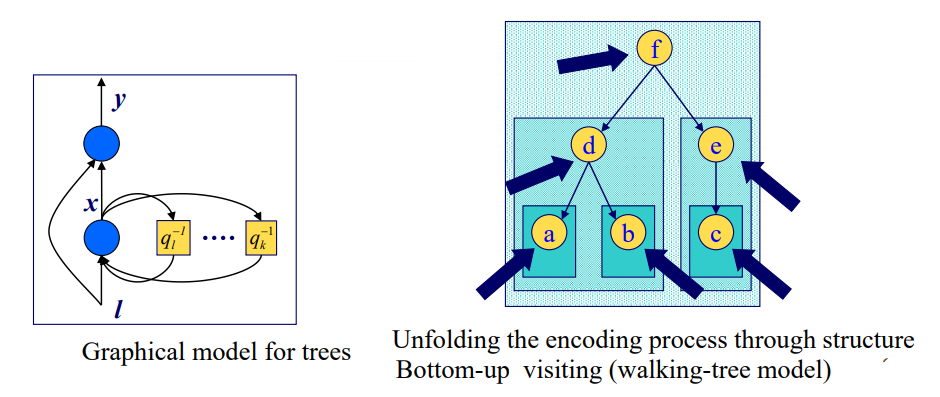
\includegraphics[scale=0.7]{42.png}
\end{center}
\paragraph{Encoding network} 
\begin{center}
	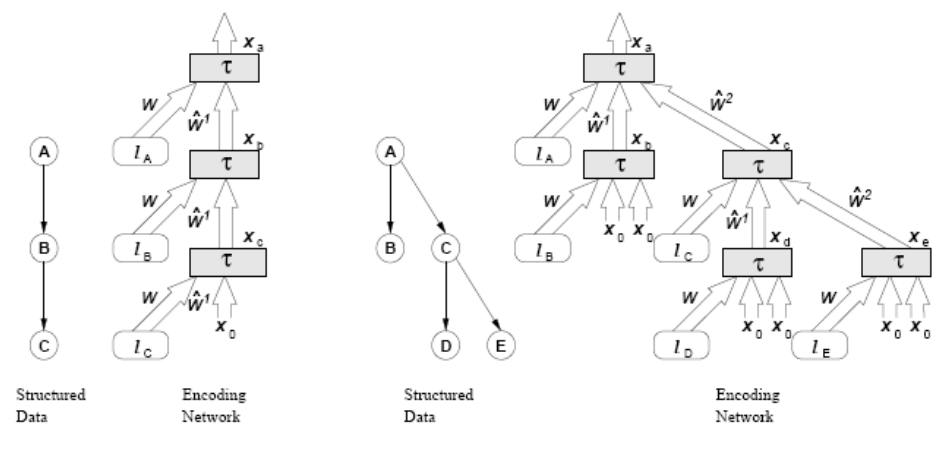
\includegraphics[scale=0.5]{43.png}
\end{center}
\textbf{Weight sharing} and \textbf{unfolding through structures}: the recursive units ($\tau$) visit all the vertexes of a tree and for all the trees in the data set.
\paragraph{Useful concepts} Recurrent neural networks transductions admit a recursive state representation with the following properties:
\begin{list}{}{}
	\item \textbf{Causality}: the transduction computed in correspondence of a vertex $v$ depends only on $v$ and its descendants
	\item \textbf{Stationarity}: the transduction computed in correspondence of a vertex $v$ is independent from the node node.\\
	$\tau$ is the same for every $v$, regardless of the dimension of sequences/structures (useful to process data of variable length with a fixed size model)
	\item \textbf{Adaptivity}: the transduction is learned from observed data
\end{list}
\subsubsection{Family of Models}
\paragraph{Recursive Cascade Correlation} Recursive Neural Networks by Recursive Cascade Correlation (RecCC), constructive approach:
\begin{list}{}{}
	\item It adds a new layer for each training step (interleaving output and hidden units training)
	\item The number of layers is automatically computed by the training algorithm
\end{list}
\begin{center}
	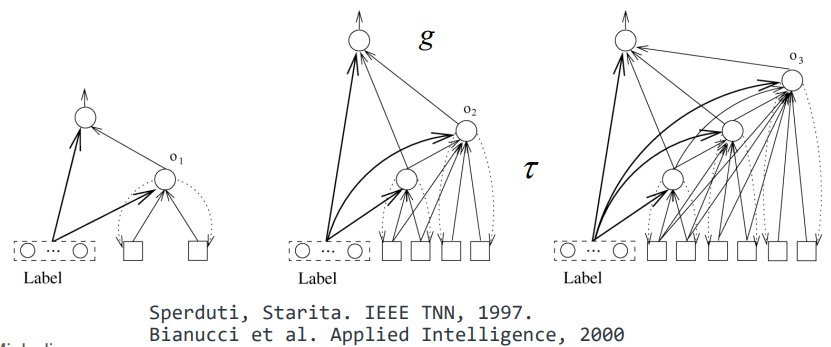
\includegraphics[scale=0.5]{44.png}
\end{center}
\paragraph{TreeESN} Combines reservoir computing (untrained reservoir layer of recurrent units with linear trained readout layer) and recursive modeling:
\begin{list}{}{}
	\item Extends the applicability of the RC/ESN approach to tree structured data
	\item Extremely efficient way of modeling RNNs (randomized approaches)
	\item Architectural and experimental performance baseline for trained RNN models with often competitive results
\end{list}
$\rightarrow$ \textbf{Deep TreeESN}: hierarchical abstraction both trough the input structure and architectural layers.
\begin{center}
	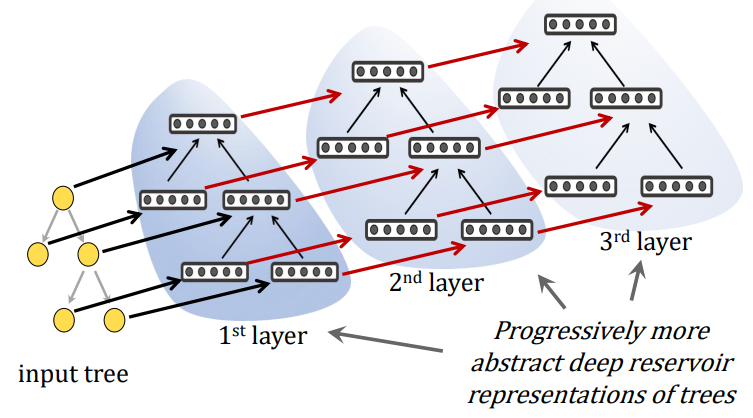
\includegraphics[scale=0.5]{45.png}
\end{center}
Improve efficiency (giving the same number of units) and improves results.
\paragraph{HTMM} For example, \textbf{Bottom-up Hidden Tree Markov models} extend HMM to trees exploiting the recursive approach. It's a generative process from the leaves to the root.\\
Uses the Markov assumption $Q$ch$_1(u),\ldots,Q$ch$_k(u)\Rightarrow Q_u$ and a children-to-parent hidden state transition\\$P(Q_u\:|\:Q$ch$_1(u),\ldots,Q$ch$_k(u))$
\begin{center}
	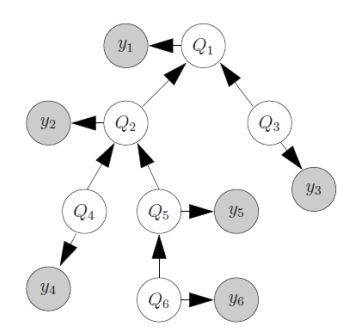
\includegraphics[scale=0.5]{46.png}
\end{center}
Bayesian network unfolding graphical model over the input trees. $y$ are the observed elements, $Q$ the hidden state variables with discrete values.
\paragraph{Unsupervised Recursive Models} Transfer recursive idea to unsupervised learning: no prior metric/preprocessing (but still bias). Evolution of the similarity measure through recursive comparison of sub-structures.\\
Iteratively compared via bottom-up encoding process.
\subsubsection{Analysis}
\paragraph{Assumptions and Open Problems} Inherited from time sequence processing. Allow adaptive representation of SD, handling of variability by causality and stationarity:
\begin{list}{}{}
	\item \textbf{Stationarity}: efficacy solution to parsimony without reducing expressive power
	\item \textbf{Causality}: affects the computational power! RNN are only able to memorize past information, outputs depend only on sub-structures and the domain is restricted to sequences and trees due to causality
\end{list}
Toward partial relaxation (or \textbf{extension}) of the causality assumption.
\paragraph{Towards Context} Kind of data domain, \textbf{contextual processing} (does the model process vertexes considering the context over the graph?), \textbf{efficiency} (often graph processing induce high complexity), \textbf{adaptivity} (including generalization performance).\\
Contextual processing can be referred to computations that yields for each vertex a response that depends on the whole information represented in the structured data, according to its topology. Causality introduces an issue: how to deal with cycles and causality? Two main approaches:\begin{list}{}{}
	\item \textbf{RNN}: explicitly treat the cycles constraining state dynamics to be contractive.\begin{list}{}{}
		\item \textbf{GraphESN/GNN}, cycles are allowed in state computation, the state is computed iterating the state transition function until convergence. Stability of the recursive encoding process is guaranteed by resorting to contractive state dynamics (banach theorem for fixed point).\\
		In GNN imposing constraints in the loss function (alternating learning and convergence), while in GraphESN the condition is inherited by contractivity of the reservoir dynamics (very efficient).
		\item \textbf{FDGNN} deep embedding: exploit embedding from the previous layer to develop a higher order embedding\begin{center}
			\includegraphics[scale=0.5]{47.png}
		\end{center}
	\end{list}
	\item \textbf{Layering}: contextual non-recursive approach. Basic idea (aka deep learning for graphs): the mutual dependencies are managed (architecturally) through different layers. Instead of iterating at the same layer, each vertex can take the context of the other vertexes computed in the previous layers, accessing progressively to the entire graph/network, and each vertex take information from all the others including mutual influences.\begin{list}{}{}
		\item \textbf{NN4G}: pioneer approach following the RNN/CRCC line (completely relaxing the recursive causality assumption). It visits the nodes of the input graphs through units with weight sharing (stationarity), i.e. we apply the same model to each node and for each node we compose the context through layers.\\
		Composition through layers. The context window is incrementally extended when the number of hidden units is decreased.
		\begin{center}
			\includegraphics[scale=0.5]{48.png}
		\end{center}
		Encoding transduction implemented by a non-recursive state transition function. Overcome the causal assumption: directly deal with cyclic/acyclic directed/undirected graphs. Contextual and constructive approach: layer by layer learning and automatic model design. This gives advantages: no gradient vanish issues, divide et impera, automatic number of layers etc (while standard CNN for graphs use end-to-end top-down backpropagation training over fixed architectures).
		\item \textbf{CNN for graphs}: moving the idea of 2D processing to graph processing through many layers.
	\end{list}
\end{list}
\subsection{Other Approaches and Other Tasks}
\subsubsection{Kernel Methods for SD}
$$k(x,x')=\langle\phi(x),\phi(x')\rangle$$
Data $x$ can be of different types, including structured data.
\paragraph{Kernel Modularity} The definition can easily be extended to graphs of different types: sequences, trees, graphs. Implicit embedding of data into euclidean space by specifying an inner product.
\paragraph{Marginalized Kernel} Similarity between two graphs based on the commod label paths obtained by random walks in the graphs. Kernel function defined as the inner product of the count vectors, averaged over all possible label paths. The computational complexity of the kernel function typically scales quadratically with the graph size.
\begin{center}
	\includegraphics[scale=0.5]{49.png}
\end{center}
\begin{list}{}{}
	\item \textbf{Efficiency}: the cost is critical (due to sub-structure decomposition)
	\item Similarity measure \textbf{fixed} prior to learning, so no adaptivity/learning in the encoding into the feature space.\begin{list}{}{}
		\item Pro: we can exploit prior knowledge with this kernel, by engineering it for a specific problem
		\item Con: for SD no universality is known $\Rightarrow$ \textbf{the choice of the kernel function is critical}\\
		E.g.: computing any complete graph kernel is at least as hard as graph isomorphism
	\end{list}
\end{list}
\subsubsection{Adaptive Kernels with Generative Models}
Represent data by feature vectors derived from generative models for structured data (e.g. HMM for sequence). Combine generative and discriminative models. The advantage is that the kernel is adapted to the dataset (data distribution).\\
Examples: fisher kernel, kernels from HTMM\ldots
\subsubsection{Statistical Relational Learning}
Combining expressive knowledge representation formalisms such as relational and first-order logic (add expressive representation to statistical approaches) with probabilistic and statistical approaches to inference and learning (add treatment of uncertainty and statistical learning to logic).\\
Typical applications:
\begin{list}{}{}
	\item Link prediction, predicting whether or not two or more objects are related
	\item Link-based clustering, grouping of similar objects where similarity is determined according to the links of a object
	\item Social network modeling
	\item Objects identification/Entity resolution
\end{list}
\subsubsection{And others\ldots}
\begin{list}{}{}
	\item Distance based (and kernel based methdos): need a priori encoding or similarity measure for structured data
	\item Subgraph mining based approaches, e.g. decomposition in substructures. Frequent subgraph patterns approaches
\end{list}
\section{Toward Research}
\paragraph{General Challenges}\begin{list}{}{}
	\item Autonomous intelligent/learning machines: robotics, HRI, search engines,\ldots
	\item Powerful tools for emerging challenges in intelligent data analysis, tools for the data scientists
	\item Innovative interdisciplinary open problems: imagination is the only limit!
\end{list}
Computational mathematics for learning and data analysis, and parallel and distributed systems $\longrightarrow$ machine learning, which $\longrightarrow$
\begin{list}{$\rightarrow$}{}
	\item Human Language technologies
	\item Intelligent Systems for Pattern Recognition
	\item Smart Applications
	\item \textbf{Computational Neuroscience}
	\item Robotics
	\item Semantic Web
	\item Algorithm Engineering
	\item Data Mining
	\item Information Retrieval
	\item Mobile and Cyber-Physical Systems
\end{list}
\end{document}
